\documentclass[11pt,titlepage]{article}

\usepackage{graphicx}
\usepackage{amsmath}

\usepackage{enumerate}
\usepackage[margin =.75in]{geometry}
\usepackage{graphicx}
\usepackage{mathtools,amssymb,amsfonts,amsthm}
\usepackage{color}
\usepackage[usenames,dvipsnames,svgnames,table]{xcolor}
\usepackage{comment}
\usepackage{multirow}
\usepackage{multicol}
\usepackage{polynom}
\usepackage{cancel}
\usepackage{tabularx}
\usepackage{tikz}
\usetikzlibrary{petri}
\usetikzlibrary{trees}
\usepackage{url}
\usepackage[linktoc=all,colorlinks=true,linkcolor=blue,urlcolor=blue,citecolor=cyan]{hyperref}
\usepackage[all]{hypcap}
\usepackage{newverbs}
\usepackage{euscript,mathrsfs}
\usepackage{pdfpages}
\usepackage{bbm}
\usepackage{parskip}
\usepackage[most]{tcolorbox}

\usepackage{cmbright}
%\usepackage[sfdefault]{atkinson}
\usepackage[T1]{fontenc}
\usepackage[italic]{mathastext}
%Cursed: Do not touch.
%\usepackage{fontspec} 
%\setmainfont{Comic Sans MS}

%\usepackage[all]{xy}
%\usepackage{wrapfig}
%\usepackage{caption}
\raggedbottom
\allowdisplaybreaks

\specialcomment{lecturenotes}{}{}\excludecomment{lecturenotes}
\specialcomment{answers}{\sss \textsc{Answer: }}{\sss}
%\excludecomment{answers} % comment to compile with answers.
\specialcomment{remarks}{

\sss
\begingroup\color{blue}}
{\endgroup

\sss}
\specialcomment{inremarks}{\begingroup\color{blue}[}{]\endgroup}
%\specialcomment{undefined}{\begingroup\color{orange}}{\endgroup}
\specialcomment{unjustified}{\begingroup\color{red}}{\endgroup}
\specialcomment{grammar}{\begingroup\color{Green}}{\endgroup}
\specialcomment{tex}{\begingroup\color{purple}}{\endgroup}

\newverbcommand{\cverb}{\small\color{purple}}{}
\newverbcommand{\everb}{\small\color{blue}}{}

\newcolumntype{L}[1]{>{\hsize=#1\hsize\raggedright\arraybackslash}X}
\newcolumntype{R}[1]{>{\hsize=#1\hsize\raggedleft\arraybackslash}X}
\newcolumntype{C}[1]{>{\hsize=#1\hsize\centering\arraybackslash}X}

\newcommand{\sss}{\vspace{2 mm}\noindent}
\newcommand{\lss}{\vspace{5 mm}\noindent}
\newcommand{\lls}{\vspace{7 mm}\noindent}
\newcommand\Tstrut{\rule{0pt}{2.6ex}}         % = `top' strut
\newcommand\Bstrut{\rule[-1ex]{0pt}{0pt}}   % = `bottom' strut
\newcommand{\ds}{\displaystyle}
\newcommand{\HR}{\vspace{5pt}\hrule height 1pt \vspace{5pt}}
\newcommand{\atext}[1]{\text{\quad #1 \quad }}

\newcommand{\Proj}[2]{\ensuremath{\mathrm{Proj}_{#2}\left({#1}\right)}}
\newcommand{\proj}[2]{\ensuremath{\mathrm{Proj}_{#2}\left({#1}\right)}}
\newcommand{\ca}{\mathcal}
\newcommand{\fr}{\mathfrak}
\newcommand{\eucal}{\EuScript}
\newcommand{\scr}{\mathscr}
\newcommand{\bbf}{\mathbb{F}}
\newcommand{\bbn}{\mathbb{N}}
\newcommand{\bbr}{\mathbb{R}}
\newcommand{\bbq}{\mathbb{Q}}
\newcommand{\bbc}{\mathbb{C}}
\newcommand{\bbz}{\mathbb{Z}}
\newcommand{\bbp}{\mathbb{P}}
\newcommand{\bfa}{\mathbf{a}}
\newcommand{\bfb}{\mathbf{b}}
\newcommand{\bfc}{\mathbf{c}}
\newcommand{\bfu}{\mathbf{u}}
\newcommand{\bfv}{\mathbf{v}}
\newcommand{\bfx}{\mathbf{x}}
\newcommand{\vca}{\vec{a}}
\newcommand{\vcb}{\vec{b}}
\newcommand{\vcc}{\vec{c}}
\newcommand{\vcd}{\vec{d}}
\newcommand{\vce}{\vec{e}}
\newcommand{\vcf}{\vec{f}}
\newcommand{\vcg}{\vec{g}}
\newcommand{\vch}{\vec{h}}
\newcommand{\vci}{\hat{i}}%i'm sorry for this gross hack but i am lazy
\newcommand{\vcj}{\hat{j}}
\newcommand{\vck}{\hat{k}}
\newcommand{\vcl}{\vec{l}}
\newcommand{\vcm}{\vec{m}}
\newcommand{\vcn}{\vec{n}}
\newcommand{\vco}{\vec{o}}
\newcommand{\vcp}{\vec{p}}
\newcommand{\vcq}{\vec{q}}
\newcommand{\vcr}{\vec{r}}
\newcommand{\vcs}{\vec{s}}
\newcommand{\vct}{\vec{t}}
\newcommand{\vcu}{\vec{u}}
\newcommand{\vcv}{\vec{v}}
\newcommand{\vcw}{\vec{w}}
\newcommand{\vcx}{\vec{x}}
\newcommand{\vcy}{\vec{y}}
\newcommand{\vcz}{\vec{z}}
\newcommand{\vcT}{\vec{T}}
\newcommand{\vcN}{\vec{N}}
\newcommand{\vcE}{\vec{E}}
\newcommand{\vcF}{\vec{F}}
\newcommand{\vcS}{\vec{S}}
\newcommand{\vomega}{\vec{\omega}}
\newcommand{\vprime}{\hspace{0.2em}'}
\newcommand{\vzero}{\vec{0}}
\newcommand{\mcl}{\mathcal{L}}
\newcommand{\mcm}{\mathcal{M}}
\newcommand{\del}{\partial}
\newcommand{\delx}[1]{\frac{\partial #1}{\partial x}}
\newcommand{\dely}[1]{\frac{\partial #1}{\partial y}}
\newcommand{\delz}[1]{\frac{\partial #1}{\partial z}}

\newcommand{\inv}{^{-1}}
\newcommand{\into}{\hookrightarrow}
\newcommand{\onto}{\twoheadrightarrow}
\newcommand{\isom}{\overset{\sim}{\to}}
\renewcommand{\iff}{\Leftrightarrow}
\renewcommand{\implies}{\Rightarrow}
\renewcommand{\impliedby}{\Leftarrow}
\newcommand{\contradiction}{\Rightarrow\Leftarrow}

\newcommand{\bmat}[1]{\begin{bmatrix}#1\end{bmatrix}}
\newcommand{\pmat}[1]{\begin{pmatrix}#1\end{pmatrix}}
\newcommand{\vmat}[1]{\begin{vmatrix}#1\end{vmatrix}}
\newcommand{\floor}[1]{\lfloor #1 \rfloor}
\newcommand{\Floor}[1]{\left\lfloor #1 \right\rfloor}
\newcommand{\vect}[1]{\langle #1 \rangle}

\newcommand{\Ad}{\operatorname{Ad}}
\newcommand{\ad}{\operatorname{ad}}
\newcommand{\disc}{\operatorname{disc}}
\newcommand{\domain}{\operatorname{domain}}
\newcommand{\Id}{\operatorname{Id}}
\newcommand{\im}{\operatorname{im}}
\newcommand{\ind}{\operatorname{ind}}
\newcommand{\nul}{\operatorname{Nul}}
\newcommand{\nullity}{\operatorname{nullity}}
\newcommand{\ord}{\operatorname{ord}}
\newcommand{\rank}{\operatorname{rank}}
\newcommand{\red}{\operatorname{red}}
\newcommand{\bbref}{\operatorname{rref}}
\newcommand{\tr}{\operatorname{tr}}
\newcommand{\trunc}{\operatorname{Trunc}}
\newcommand{\vspan}{\operatorname{span}}
\newcommand{\cl}{\operatorname{cl}}
\newcommand{\bd}{\operatorname{bd}}
\newcommand{\inte}{\operatorname{int}}
\newcommand{\sub}{\operatorname{sub}}
\newcommand{\sgn}{\operatorname{sgn}}
\newcommand{\fix}{\operatorname{Fix}}
\newcommand{\syl}{\operatorname{Syl}}
\newcommand{\aut}{\operatorname{Aut}}
\newcommand{\curl}{\operatorname{Curl}}
\newcommand{\divo}{\operatorname{Div}}
\newcommand{\de}{^\circ}
%\theoremstyle{definition}
\newtheorem{thm}{Theorem}[section]
\newtheorem{prop}[thm]{Proposition}
\newtheorem{cor}[thm]{Corollary}
\newtheorem{lem}[thm]{Lemma}
\newtheorem*{prop*}{Proposition}
\newtheorem*{cor*}{Corollary}
\newtheorem*{lem*}{Lemma}
\newtheorem*{thm*}{Theorem}

\theoremstyle{definition}
\newtheorem{conj}[thm]{Conjecture}
\newtheorem{defn}[thm]{Definition}
%\newtheorem{claim}[thm]{Claim}
%\newtheorem{example}{}[thm]{example}{}
\newtheorem*{practice}{Practice}
\newtheorem*{conj*}{Conjecture}
\newtheorem*{rd}{Read from the text}
 \newcounter{counter}[subsection]
\newcommand*\dif{\mathop{}\!\mathtt{d}}

\setcounter{tocdepth}{3}  %How many levels to include in TOC
\addtocontents{toc}{\protect\sloppy}    %Keeps long chapters within page # margins
%%--------Solutions------%%

\newcommand{\solushun}[2]{
   
   \ifnum\showsolutions=1
       \hrulefill \\
       {\bf A Solution:}
       #1 \vspace*{\baselineskip}
       \hrulefill
   \fi
 
   \ifnum\showsolutions=0 \vspace*{#2}
   \fi
}

%%-------------AnswerKey----%%
 %\Newassociation{solution}{Soln}{AnswerKey}

% \renewcommand{\Solnlabel}[1]{\bf Exercise ~\thesubsection.#1.}

\newcommand{\AnswerKeyEntry}[1]{\Writetofile{AnswerKey}{
{\noindent \bf Exercise ~\thesubsection.\thecounter} #1 \newline \newline } }

%%-----ColorBox----------%%
\newtcolorbox{moretbox}[2][]{colback=black!50,
colframe=black!75!black,fonttitle=\bfseries,colbacktitle=gray!10,coltitle=black,enhanced,attach boxed title to top left={yshift=-2mm,xshift=5mm},title=#2,#1}

       \tcbset{colframe=black!50,colback=white,colupper=black,
	fonttitle=\bfseries,nobeforeafter,center title}


%%----EXAMPLE---------%%

    \newenvironment{example}[1]{\refstepcounter{counter}
    \medskip
    \vspace*{.05in}
    \noindent
\begin{moretbox}[breakable,colback=white,colbacktitle=gray!5]{\textbf{Example~\thesubsection.\thecounter. #1}}
\medskip } 
 { \medskip
\end{moretbox} \medskip
   }
   
%%----Claim---------%%

    \newenvironment{claim}[1]{\refstepcounter{counter}
    \medskip
    \vspace*{.05in}
    \noindent
\begin{moretbox}[breakable,colback=white,colbacktitle=gray!5]{\textbf{Claim~\thesubsection.\thecounter. #1}}
\medskip } 
 { \medskip
\end{moretbox} \medskip
   }
   
%%----Proof---------%%

    \newenvironment{pf}[1]{\refstepcounter{counter}
    \medskip
    \vspace*{.05in}
    \noindent
\begin{moretbox}[breakable,colback=white,colbacktitle=gray!5]{\textbf{Proof~\thesubsection.\thecounter. #1}}
\medskip } 
 { \medskip
\end{moretbox} \medskip
   }
   
%%----EXERCISE---------%%   

\newenvironment{exercise}[1]{\refstepcounter{counter}  
    \medskip 
    \vspace*{.05in}
    \noindent
\begin{moretbox}[breakable,colback=white,colbacktitle=gray!35]{\textbf{Exercise~\thesubsection.\thecounter. #1}}
\medskip } 
 { \medskip 
\end{moretbox} \medskip
   }      
%%----EXERCISE---------%%   

\newenvironment{pexercise}[1]{\refstepcounter{counter}  
    \medskip 
    \vspace*{.05in}
    \noindent
\begin{moretbox}[breakable,colback=white,colbacktitle=gray!35]{\textbf{Exercise~\thesubsection.\thecounter. #1\hyperlink{PON}{$^\text{P}$}}}
\medskip } 
 { \medskip 
\end{moretbox} \medskip
   }   
%%----REVEXERCISE---------%%   

\newenvironment{revex}[1]{\refstepcounter{counter}  
    \medskip 
    \vspace*{.05in}
    \noindent
\begin{moretbox}[breakable,colback=white,colbacktitle=gray!35]{\textbf{Exercise~\thecounter. #1}}
\medskip } 
 { \medskip 
\end{moretbox} \medskip
   }
%%----THEOREM---------%%
    \newenvironment{theorem}[1]{\refstepcounter{counter}  
    \medskip     
    \vspace*{.05in}
    \noindent
\begin{moretbox}[colback=white,colbacktitle=gray!5]{\textbf{Theorem~\thesubsection.\thecounter. #1}}
\medskip } 
 { \medskip
\end{moretbox} \medskip
   }
   
%%----DEFINITION---------%%

    \newenvironment{definition}[1]{\refstepcounter{counter}  
    \medskip 
    \vspace*{.05in}
    \noindent
\begin{moretbox}[colback=white,colbacktitle=gray!5]{\textbf{Definition~\thesubsection.\thecounter. #1}}
\medskip } 
 { \medskip
\end{moretbox} \medskip
   }

%%------Formula Boxes---------%%
\newcommand{\FormulaBox}[2]{
\begin{center}
\tcbox[left=0mm,right=0mm,top=0mm,bottom=0mm,boxsep=0mm,toptitle=0.5mm,bottomtitle=0.5mm,center title,title=#1]
{
	\renewcommand*{\arraystretch}{1.8} 
  #2
}
\end{center}}
\newenvironment{answer}{

\sss
\textsc{Answer:}}{\hfill $\square$

\sss}
\def\width{10}
\def\hauteur{10}
\newenvironment{prompt}{\begin{center}\begin{tikzpicture}[scale=.8, x=1cm, y=1cm, semitransparent]
%\draw[step=1mm, line width=0.1mm, black!20!white] (0,0) grid (\width,\hauteur);
%\draw[step=5mm, line width=0.2mm, black!30!white] (0,0) grid (\width,\hauteur);
\draw[step=5cm, line width=0.5mm, black!50!white] (0,0) grid (\width,\hauteur);
\draw[step=1cm, line width=0.3mm, black!70!white] (0,0) grid (\width,\hauteur);
\end{tikzpicture}\end{center}}{

\sss}
\newcounter{homework}
\newtheorem{hw}[homework]{Homework}

\newcounter{exercise}[homework]
\newtheorem{exer}[exercise]{Exercise}
\renewcommand{\theexercise}{\arabic{homework}.\arabic{exercise}}

\theoremstyle{remark}
\newtheorem*{defn*}{Definition}
\newtheorem{remark}[thm]{Remark}
\newtheorem*{remark*}{Remark}
\newtheorem{notation}[thm]{Notation}
\title{Calculus III \\ Lecture Notes and Practice}
\author{Aaron Allen}
\date{}
\begin{document}

    \begin{titlepage}
    \centering 
    \vspace*{.5in}
    {\Huge \bf Calculus III\par}
    \vspace{1.5cm}
    {\Large\itshape Aaron Allen \par}


    \vfill
    
\includegraphics[width=.4\textwidth]{Figures/FRCCLogo}\par\vspace{1cm}
    
 \vfill
 
 \begin{tabular}{c p{0.6\linewidth}c p{0.4\linewidth}} \hspace*{.5in}
 & \vspace*{.01in} This work is licensed under a Creative Commons Attribution-NonCommercial-ShareAlike 4.0 International License. &\hspace*{.1in} & \vspace*{.01in} \href{https://creativecommons.org/licenses/by-nc-sa/4.0/}{
\includegraphics{Figures/CreativeCommonsLicense}}
 \end{tabular}
 
    \end{titlepage}
\tableofcontents
\pagebreak

\section*{Notes About Notes}
Welcome to Calculus III! These notes and practice problems are intended to form a large proportion of the coursework for this course. This text is by no means a \textit{complete} reference on multivariable Calculus. Instead, the text is meant as a specific companion for our specific course, without extra overhead. If you would like an outside reference, my suggestion would to be either to pick up an old edition of Stewart's Calculus from a used books seller (this should be pretty cheap!), or to use \href{https://tutorial.math.lamar.edu/Classes/CalcIII/CalcIII.aspx}{Paul's Online Math Notes}.

A few notes on the notes:

\begin{itemize}
\item The text is designed around a course in 3 parts. 

\begin{enumerate}
\item The first part is chapters 1, 2 and 3, which cover an introduction to vectors and Calculus on functions that have vector inputs.
\item The second part is chapters 4 and 5, which cover partial derivatives and multiple integrals, or Calculus on functions that have vector outputs.
\item The third part is chapters 6 and 7, which cover line and surface integrals, or Calculus on functions with vector inputs and outputs.
\end{enumerate}

Each part has an associated exam review. Each chapter also includes a section with homework and miscellaneous practice, labeled with an R.

\item This text uses hyperlinks throughout. Some hyperlinks are internal (the table of contents links to the respective sections) and some are external (some exercises and examples have links to Geogebra for visualization). Unfortunately, this functionality is at least partially lost in a paper version of the text if you choose to print it out.
\item The text includes both examples and exercises. Any exercise that requires interaction is denoted with a slightly darker coverplate. For example:

\begin{example}{An Example of an Example}
Examples, definitions, theorems and claims look like this!
\end{example}

\begin{exercise}{An Example of an Exercise}
Exercises look like this!
\end{exercise}

\item \hypertarget{PON} Some exercises or examples are adapted from \href{https://tutorial.math.lamar.edu/Classes/CalcIII/CalcIII.aspx}{Paul's Online Math Notes}. When an exercise is adapted this way, it will be denoted with a small P in the title, as below:

\begin{pexercise}{An Example of an Exercise, Adapted}
This example would have been adapted from \href{https://tutorial.math.lamar.edu/Classes/CalcIII/CalcIII.aspx}{Paul's Online Math Notes}. 
\end{pexercise}

\item These notes are OER (open education resources) and should be available for free. You can access the \href{https://www.overleaf.com/read/qyqfjbgpysqx}{LaTeX source code here}.

%\item The notes are currently typeset in the \href{https://brailleinstitute.org/freefont}{Atkinson Hyperlegible Font} from the Braille Institute. The intention is to enhance readability for readers with low or impaired vision.
\end{itemize}

If you have any questions, concerns or comments, please reach out to me by email!

Aaron Allen, Front Range Community College
\begin{verbatim}
aaron.allen@frontrange.edu
\end{verbatim}

\section{Vector Operations and Properties}
\subsection{Vector Notation and Introduction}
Your previous journeys into Calculus so far have been generally restricted to experimentation with just $\bbr$, the set of real numbers. You have mastered (hopefully!) derivatives and integrals of functions $f:\bbr\to\bbr$ that take a single real number to a second real number. Calculus III expands on this idea by introducing \textbf{vectors}, which are essentially ordered lists of real numbers.

\begin{definition}{$n$-Dimensional Real Euclidean Space}
Define \textbf{$n$-dimensional real Euclidean space} to be the set of all lists of exactly $n$ real numbers. In set builder notation, $$\mathbb{R}^n=\left\lbrace \begin{bmatrix} a_1 \\ a_2 \\ \vdots \\ a_n\end{bmatrix}:a_i\in\bbr\right\rbrace, $$ where $n\in\bbn$ or $n$ is a natural number.
\end{definition}

\begin{definition}{Vector}
A single element of $n$-dimensional real Euclidean space is called a \textbf{vector} and usually written with a short arrow above it. For example, $$\vcv=\bmat{x\\y\\z}$$ would describe a vector in $\bbr^3$. While vertical vectors are often the best for us, to save space you will occasionally see vectors written horizontally with parentheses or angle brackets, that is:
$$\vcv=\bmat{x\\y\\z}=(x,y,z)=\langle x,y,z\rangle$$ all represent the same vector!
\end{definition}

We actually need quite a bit of \textit{linear algebra} to accurately define the definition of the term \textbf{dimension}, but it's important enough that we'll give an informal definition here.

\begin{definition}{Dimension}
The \textbf{dimension} of a vector space is the number of values needed to exactly describe an object in that vector space. The \textbf{dimension} of a vector is the dimension of the vector space that that vector lives in.
\end{definition}

Note that the dimension of $\bbr^n$ is $n$, since we need a list of $n$ real numbers to exactly describe a single vector in $\bbr^n$.

We typically draw vectors in $n$-dimensional Euclidean space as arrows, where the tail of the arrow lies on the origin and the tip of the arrow lies at the point whose coordinates are exactly said vector.

\begin{example}{$n=2$}
Let $\vcv$ and $\vcu$ be vectors in $\bbr^2$, and $\vcv=\bmat{3\\1}$ and $\vcu=\bmat{2\\-2}$. Then we draw $\vcv$ and $\vcu$ in the Euclidean plane as below:

\begin{center}
\begin{tikzpicture}[scale=.7, x=1cm, y=1cm, semitransparent]
	%\draw[step=1mm, line width=0.1mm, black!20!white] (0,0) grid (\width,\hauteur);
	%\draw[step=5mm, line width=0.2mm, black!90!white] (0,0) grid (\width,\hauteur);
	\draw[step=5cm, line width=0.5mm, black!90!white] (0,0) grid (\width,\hauteur);
	\draw[step=1cm, line width=0.2mm, black!50!white] (0,0) grid (\width,\hauteur);
	\draw[->, color=blue,line width=0.5mm](5,5)--(8,6);
	\node[color=blue] (v) at (6,6){$\vcv$};
	\draw[->, color=red, line width=0.5mm](5,5)--(7,3);
	\node[color=red] (u) at (5.6,3.8){$\vcu$};
	\end{tikzpicture}\end{center}
\end{example}
\subsection{Basic Vector Operations}
We have a few vector operations that are worth mentioning. We start with what are called ``unary" operators, or operations that only require a single input. Examples of unary operators on the real numbers are negation (i.e. turning $4$ into $-4$), or reciprocation (i.e. turning $4$ into $1/4$). The first unary operator we'll look at for vectors is \textbf{magnitude}.

\begin{definition}{Magnitude}
Let $\vcv$ be an $n$-dimensional vector, that is $\vcv=\bmat{v_1\\v_2\\ \vdots \\ v_n}$. Then the magnitude of $\vcv$ is: $$||\vcv||=\sqrt{v_1^2+v_2^2+\cdots+v_n^2}. $$
\end{definition}

\begin{exercise}{Magnitudes}
Find the magnitude for the following vectors:
\begin{enumerate}
\item $\vcv=(1,4)$
\vspace{1em}
\item $\vcu=(3,-2)$
\vspace{1em}
\item $\vca=(3,1,-2)$
\vspace{1em}
\item $\vcb=(6,2,-4,12)$
\end{enumerate}
\end{exercise}

A related definition is that of the \textbf{unit vector}. Technically you can think of this as a unary operation that takes a vector and returns the unit version of that vector.

\begin{definition}{Unit Vector}
We say that $\vcv$ is a \textbf{unit} vector if $||\vcv||=1$. We can find a unit vector that is parallel (has the same direction) of $\vcv$ by dividing $\vcv$ by its own magnitude. That is: $$\hat{v}=\frac{1}{||\vcv||}\vcv.$$
\end{definition}

\begin{definition}{Zero Vector}
We say that $\vcv$ is the \textbf{zero} vector if $||\vcv||=0$, and we write $\vcv=\vzero$.
\end{definition}

The second important unary operation is \textbf{negation}. 

\begin{definition}{Vector Negation}
Let $\vcv\in\bbr^n$, that is, $\vcv=\bmat{v_1\\v_2\\ \vdots \\ v_n}$. Then $-\vcv=\bmat{-v_1\\-v_2\\ \vdots \\ -v_n}$.
\end{definition}

Then that brings us into our second category of operations, ``binary" operators, or operators that require two inputs. Examples of binary operators on real numbers are addition, multiplication, etc. We see analogues for these for vectors in vector addition and scalar multiplication.

\begin{definition}{Vector Addition}
Let $\vcv$ and $\vcu$ be two vectors in $\bbr^n$. Then to add these two vectors, we add the corresponding coordinates. That is,
$$\vcv\pm \vcu=\bmat{v_1\\v_2\\ \vdots\\v_n}\pm\bmat{u_1\\u_2\\ \vdots\\u_n}=\bmat{v_1\pm u_1\\v_2\pm u_2\\ \vdots\\v_n\pm u_n}. $$
\end{definition}

\begin{definition}{Scalar Multiplication}
Given a vector $\vcv$ in $\bbr^n$ and a number $c$ in $\bbr$ (called a scalar), their product is defined by distributing the scalar to each coordinate of the vector. That is,
$$c\vcv=c\bmat{v_1\\v_2\\ \vdots\\v_n}=\bmat{cv_1\\cv_2\\ \vdots \\ c v_n}.$$
\end{definition}

The way we add vectors is ``timewise". Vectors are typically drawn as arrows with a length(magnitude) and direction. If we place the tail of the vector $\vcv=(x,y)$ on the origin, the tip of the arrow would land at the point $(x,y)$. 

\begin{center}
\begin{tikzpicture}[scale=.7, x=1cm, y=1cm, semitransparent]
	%\draw[step=1mm, line width=0.1mm, black!20!white] (0,0) grid (\width,\hauteur);
	%\draw[step=5mm, line width=0.2mm, black!90!white] (0,0) grid (\width,\hauteur);
	\draw[step=5cm, line width=0.5mm, black!90!white] (0,0) grid (\width,\hauteur);
	\draw[step=1cm, line width=0.2mm, black!50!white] (0,0) grid (\width,\hauteur);
	\draw[->, color=blue,line width=0.5mm](5,5)--(7.6,6);
	\node[color=blue] (v) at (6,6){$\vcv$};
	\draw[->, color=red, line width=0.5mm](5,5)--(7,3.6);
	\node[color=red] (u) at (5.6,3.8){$\vcu$};
	\end{tikzpicture}\end{center}

Geometrically, to add two vectors, we follow one, then follow the other. That is, we place them tail to tip:

\begin{center}
\begin{tikzpicture}[scale=.7, x=1cm, y=1cm, semitransparent]
	%\draw[step=1mm, line width=0.1mm, black!20!white] (0,0) grid (\width,\hauteur);
	%\draw[step=5mm, line width=0.2mm, black!90!white] (0,0) grid (\width,\hauteur);
	\draw[step=5cm, line width=0.5mm, black!90!white] (0,0) grid (\width,\hauteur);
	\draw[step=1cm, line width=0.2mm, black!50!white] (0,0) grid (\width,\hauteur);
	\draw[->, color=blue,line width=0.5mm](5,5)--(7.6,6);
	\node[color=blue] (v) at (6,6){$\vcv$};
	\draw[->, color=red, line width=0.5mm](7.6,6)--(9.6,4.6);
	\node[color=red] (u) at (8.5,6){$\vcu$};
	\draw[->,color=violet,line width=0.5mm](5,5)--(9.6,4.6);
	\node[color=violet](uv) at (7.3, 4.5){$\vcv+\vcu$};
	\draw[->, color=red, line width=0.5mm](5,5)--(7,3.6);
	\node[color=red] (u1) at (5.6,3.8){$\vcu$};
	\draw[->, color=blue,line width=0.5mm](7,3.6)--(9.6,4.6);
	\node[color=blue] (v1) at (8.5,3.5){$\vcv$};
	\end{tikzpicture}\\
	For a 3d example, look \href{https://www.geogebra.org/3d/kdfbhfvx}{here}.\end{center}

Note, commutativity holds! If we follow $\vcv$ first, then $\vcu$, we end up at the same spot as if we followed $\vcu$ first then $\vcv$. In fact, this makes a parallelogram. 

The vector drawn from the starting point to the ending point is exactly the sum of the two vectors. The difference of two vectors can be found from the same triangle as the sum:

\begin{center}
\begin{tikzpicture}[scale=.7, x=1cm, y=1cm, semitransparent]
	%\draw[step=1mm, line width=0.1mm, black!20!white] (0,0) grid (\width,\hauteur);
	%\draw[step=5mm, line width=0.2mm, black!90!white] (0,0) grid (\width,\hauteur);
	\draw[step=5cm, line width=0.5mm, black!90!white] (0,0) grid (\width,\hauteur);
	\draw[step=1cm, line width=0.2mm, black!50!white] (0,0) grid (\width,\hauteur);
	\draw[->, color=blue,line width=0.5mm](5,5)--(7.6,6);
	\node[color=blue] (v) at (6,6){$\vcv$};
	\draw[->, color=red, line width=0.5mm](5,5)--(7,3.6);
	\node[color=red] (u) at (5.6,3.8){$\vcu$};
	\draw[->, color=violet, line width=0.5mm](7.6,6)--(7,3.6);
	\node[color=violet] (w) at (8.6,4.5){$\vcw=\vcu-\vcv$};
	\end{tikzpicture}\\
	For a 3d example, look \href{https://www.geogebra.org/3d/zqhabgw9}{here}.\end{center}

Here, $\vcv+\vcw=\vcu$. Then it follows that $\vcu-\vcv=\vcw$. That is, the difference between two vectors is the vector that goes from the tip of the second (``negative") vector to the tip of the second (``positive") vector.

\index{Vector!Scalar Multiplication}To multiply a vector by a scalar, we just scale the vector. In other words, the magnitude of the vector increases or decreases. For example:
\begin{center}
\begin{tikzpicture}[scale=.5, x=1cm, y=1cm, semitransparent]
	%\draw[step=1mm, line width=0.1mm, black!20!white] (0,0) grid (\width,\hauteur);
	%\draw[step=5mm, line width=0.2mm, black!90!white] (0,0) grid (\width,\hauteur);
	\draw[step=5cm, line width=0.5mm, black!90!white] (0,0) grid (\width,\hauteur);
	\draw[step=1cm, line width=0.2mm, black!50!white] (0,0) grid (\width,\hauteur);
	\draw[->, color=red, line width=0.5mm](5,5)--(7,3.6);
	\node[color=red] (u) at (5.6,3.8){$\vcu$};
	\end{tikzpicture}
	\begin{tikzpicture}[scale=.5, x=1cm, y=1cm, semitransparent]
	%\draw[step=1mm, line width=0.1mm, black!20!white] (0,0) grid (\width,\hauteur);
	%\draw[step=5mm, line width=0.2mm, black!90!white] (0,0) grid (\width,\hauteur);
	\draw[step=5cm, line width=0.5mm, black!90!white] (0,0) grid (\width,\hauteur);
	\draw[step=1cm, line width=0.2mm, black!50!white] (0,0) grid (\width,\hauteur);
	\draw[->, color=red, line width=0.5mm](5,5)--(9,2.2);
	\node[color=red] (u) at (7,3){$2\vcu$};
	\end{tikzpicture}\end{center}

If that scalar is negative, the direction of the vector reverses! This is similar to how negative numbers go in the opposite direction of positive numbers along the number line. Another way of verifying this is that if you add $\vcv+(-\vcv)$, you should get the 0 vector, $\vzero$! In $\bbr\times \bbr$, $\vzero=(0,0)$. 
\begin{center}
\begin{tikzpicture}[scale=.5, x=1cm, y=1cm, semitransparent]
	%\draw[step=1mm, line width=0.1mm, black!20!white] (0,0) grid (\width,\hauteur);
	%\draw[step=5mm, line width=0.2mm, black!90!white] (0,0) grid (\width,\hauteur);
	\draw[step=5cm, line width=0.5mm, black!90!white] (0,0) grid (\width,\hauteur);
	\draw[step=1cm, line width=0.2mm, black!50!white] (0,0) grid (\width,\hauteur);
	\draw[->, color=red, line width=0.5mm](5,5)--(7,3.6);
	\node[color=red] (u) at (5.6,3.8){$\vcu$};
	\end{tikzpicture}
	\begin{tikzpicture}[scale=.5, x=1cm, y=1cm, semitransparent]
	%\draw[step=1mm, line width=0.1mm, black!20!white] (0,0) grid (\width,\hauteur);
	%\draw[step=5mm, line width=0.2mm, black!90!white] (0,0) grid (\width,\hauteur);
	\draw[step=5cm, line width=0.5mm, black!90!white] (0,0) grid (\width,\hauteur);
	\draw[step=1cm, line width=0.2mm, black!50!white] (0,0) grid (\width,\hauteur);
	\draw[->, color=red, line width=0.5mm](5,5)--(1,7.8);
	\node[color=red] (u) at (3.5,7.5){$-2\vcu$};
	\end{tikzpicture}\end{center}
	Here, $-2\vcu$ is in the opposite direction of $\vcu$, and twice as long!
	
\begin{exercise}{Operating on Vectors Geometrically}
Let $\vec{v}=(2,3), \vec{u}=(1,-1)$
\begin{itemize}
\vspace{1em}

\item On axes below, draw and label the vectors $\vec{v}$ and $\vec{u}$. The tails of the vectors should be at the origin!

\begin{center}\begin{tikzpicture}[scale=.5, x=1cm, y=1cm, semitransparent]
	%\draw[step=1mm, line width=0.1mm, black!20!white] (0,0) grid (\width,\hauteur);
	%\draw[step=5mm, line width=0.2mm, black!90!white] (0,0) grid (\width,\hauteur);
	\draw[step=5cm, line width=0.5mm, black!90!white] (0,0) grid (\width,\hauteur);
	\draw[step=1cm, line width=0.2mm, black!90!white] (0,0) grid (\width,\hauteur);
	\end{tikzpicture}\end{center}
	
\item On axes below, show how to combine the two vectors to get $\vcv+\vcu$. Approximate the value of the sum.
\begin{center}\begin{tikzpicture}[scale=.5, x=1cm, y=1cm, semitransparent]
	%\draw[step=1mm, line width=0.1mm, black!20!white] (0,0) grid (\width,\hauteur);
	%\draw[step=5mm, line width=0.2mm, black!90!white] (0,0) grid (\width,\hauteur);
	\draw[step=5cm, line width=0.5mm, black!90!white] (0,0) grid (\width,\hauteur);
	\draw[step=1cm, line width=0.2mm, black!90!white] (0,0) grid (\width,\hauteur);
	\end{tikzpicture}\end{center}
\item On axes below, show how to combine the two vectors to get $\vcv-\vcu$. Approximate the value of the difference.
\begin{center}\begin{tikzpicture}[scale=.5, x=1cm, y=1cm, semitransparent]
	%\draw[step=1mm, line width=0.1mm, black!20!white] (0,0) grid (\width,\hauteur);
	%\draw[step=5mm, line width=0.2mm, black!90!white] (0,0) grid (\width,\hauteur);
	\draw[step=5cm, line width=0.5mm, black!90!white] (0,0) grid (\width,\hauteur);
	\draw[step=1cm, line width=0.2mm, black!90!white] (0,0) grid (\width,\hauteur);
	\end{tikzpicture}\end{center}
	\pagebreak
\item On axes below, show how to scale a vector to get $3\vcu$. Approximate the value of $3\vcu$.
\begin{center}\begin{tikzpicture}[scale=.5, x=1cm, y=1cm, semitransparent]
	%\draw[step=1mm, line width=0.1mm, black!20!white] (0,0) grid (\width,\hauteur);
	%\draw[step=5mm, line width=0.2mm, black!90!white] (0,0) grid (\width,\hauteur);
	\draw[step=5cm, line width=0.5mm, black!90!white] (0,0) grid (\width,\hauteur);
	\draw[step=1cm, line width=0.2mm, black!90!white] (0,0) grid (\width,\hauteur);
	\end{tikzpicture}\end{center}
\item On axes below, show how to scale a vector to get $-\vcv$. Approximate the value of $-\vcv$.
\begin{center}\begin{tikzpicture}[scale=.5, x=1cm, y=1cm, semitransparent]
	%\draw[step=1mm, line width=0.1mm, black!20!white] (0,0) grid (\width,\hauteur);
	%\draw[step=5mm, line width=0.2mm, black!90!white] (0,0) grid (\width,\hauteur);
	\draw[step=5cm, line width=0.5mm, black!90!white] (0,0) grid (\width,\hauteur);
	\draw[step=1cm, line width=0.2mm, black!90!white] (0,0) grid (\width,\hauteur);
	\end{tikzpicture}\end{center}
\end{itemize}
\end{exercise}

\begin{exercise}{}
Find the following:
\begin{enumerate}
\item $(1,4)+(3,2)=$
\vspace{1em}
\item $3(2,3)-2(-1,6)=$
\end{enumerate}
\end{exercise}

Note that we can write vectors in an alternative way using what are called \textbf{elementary basis vectors}.

\begin{definition}{Elementary Basis Vectors in $\bbr^2$ and $\bbr^3$}
In $\bbr^2$, we define two \textbf{elementary basis vectors} as $$\hat{i}=\bmat{1\\0},\ \hat{j}=\bmat{0\\1}.$$
In $\bbr^3$, we define three \textbf{elementary basis vectors} as $$\hat{i}=\bmat{1\\0\\0},\ \hat{j}=\bmat{0\\1\\0},\ \hat{k}=\bmat{0\\0\\1}. $$
\end{definition}

We can decompose vectors into sums of elementary basis vectors:

\begin{example}{}
Let $$\vcv=\bmat{4\\-3\\2}.$$ Then we can write 
\begin{align*}
\vcv=&\bmat{4\\0\\0}+\bmat{0\\-3\\0}+\bmat{0\\0\\2}\\
=&4\bmat{1\\0\\0}-3\bmat{0\\1\\0}+2\bmat{0\\0\\1}\\
=&4\hat{i}-3\hat{j}+2\hat{k}.
\end{align*}
\end{example}
\subsection{Dot Product}

You may have noticed that while we can add and subtract vectors, and we can multiply them by scalars, there is no allowance for multiplying or dividing two vectors. In general, there is no requirement for a well-defined product of two vectors in a vector space. However, there are a couple of useful ``product" operations that show up with real-valued vectors. One of these is called the \textbf{dot product}.

\begin{definition}{Definition of Dot Product}
Let $\vcv$ and $\vcw$ be two vectors in $\bbr^n$. Then the \textbf{dot product} of $\vcv$ and $\vcw$ is defined as:
\begin{align*}
\vcv\bullet\vcw=&\sum_{i=1}^n v_i w_i \\
=&v_1 w_1 + v_2 w_2 +\cdots+v_n w_n 
\end{align*}
\end{definition}

\begin{exercise}{}
Find the following dot products:
\begin{enumerate}
\item $(3,2)\bullet(2,7)$
\vspace{1em}
\item $(1,2,3)\bullet(-2,3,1) $
\vspace{1em}
\item $(2,6,-4,-1)\bullet(-1,3,-4,2)$
\vspace{1em}
\item $(3,-14,12)\bullet(-24,21,3)$
\vspace{1em}
\end{enumerate}
\end{exercise}

% The vector drawn from the starting point to the ending point is exactly the sum of the two vectors. The difference of two vectors can be found from the same triangle as the sum:

% \begin{center}
% \begin{tikzpicture}[scale=.7, x=1cm, y=1cm, semitransparent]
% 	%\draw[step=1mm, line width=0.1mm, black!20!white] (0,0) grid (\width,\hauteur);
% 	%\draw[step=5mm, line width=0.2mm, black!90!white] (0,0) grid (\width,\hauteur);
% 	\draw[step=5cm, line width=0.5mm, black!90!white] (0,0) grid (\width,\hauteur);
% 	\draw[step=1cm, line width=0.2mm, black!50!white] (0,0) grid (\width,\hauteur);
% 	\draw[->, color=blue,line width=0.5mm](5,5)--(7.6,6);
% 	\node[color=blue] (v) at (6,6){$\vcv$};
% 	\draw[->, color=red, line width=0.5mm](5,5)--(7,3.6);
% 	\node[color=red] (u) at (5.6,3.8){$\vcu$};
% 	\draw[->, color=violet, line width=0.5mm](7.6,6)--(7,3.6);
% 	\node[color=violet] (w) at (7.8,4.5){$\vcw$};
% 	\end{tikzpicture}\end{center}

% Here, $\vcv+\vcw=\vcu$. Then it follows that $\vcu-\vcv=\vcw$. That is, the difference between two vectors is the vector that goes from the tip of the second (``negative") vector to the tip of the second (``positive") vector.

\begin{exercise}{The Law of Cosines and the Dot Product}
Sometimes, given two vectors $\vcv=(v_1,v_2)$, $\vcw=(w_1,w_2)$ with angle $\theta$ between them the expression $$\vcv\bullet\vcw=||\vcv|| \ ||\vcw||\cos\theta. $$ is referred to as ``the dot product version of the law of cosines". Why? Let's find out. We'll start by constructing a vector triangle, placing $\vcv$ and $\vcw$ in standard position:
\begin{center}
\begin{tikzpicture}[scale=.7, x=1cm, y=1cm, semitransparent]
	%\draw[step=1mm, line width=0.1mm, black!20!white] (0,0) grid (\width,\hauteur);
	%\draw[step=5mm, line width=0.2mm, black!90!white] (0,0) grid (\width,\hauteur);
	\draw[step=5cm, line width=0.5mm, black!90!white] (-5,-5) grid (4.99,4.99);
	%\draw[step=1cm, line width=0.2mm, black!50!white] (-5,-5) grid (5,5);
	\draw[->, color=blue,line width=0.5mm](0,0)--(30:4);
	\node[color=blue] (v) at (1.25,1.5){$\vcv$};
	\draw[->, color=red, line width=0.5mm](0,0)--(320:3);
	\node[color=red] (u) at (.75,-1.25){$\vcw$};
	\draw[->, color=violet, line width=0.5mm](320:3)--(30:4);
        \draw[line width=0.5mm] (320:1) arc (-40:30:1);
        \node (theta) at (-15:1.25){$\theta$};
	%\node[color=violet] (w) at (7.8,4.5){$\vcw$};
	\end{tikzpicture}\end{center}
	\begin{itemize}
	\item What is the purple vector (from the tip of $\vcw$ to the tip of $\vcv$)? Hint: Think about the geometric difference of two vectors.
	\vspace{5em}
	\item What are the lengths of the three sides of this triangle? Hint: The length of a vector is its \textbf{magnitude}.
	\vspace{5em}
	\item Using the Law of Cosines, write an expression relating your three side lengths and $\theta$.
	\vspace{10em}
	\item Show that this expression simplifies to $$\vcv\bullet\vcw=||\vcv|| \ ||\vcw||\cos\theta. $$
	Hint: Leave $-2||\vcv|| \ ||\vcw||\cos\theta$ alone for now, but expand out all of the other magnitudes using the magnitude formula, expand, then see if anything cancels.
	\vspace{50em}
	\end{itemize}
\end{exercise}

Note that this rule $$\vcv\bullet\vcw=||\vcv|| \ ||\vcw||\cos\theta$$ does \textit{not} just hold in $\bbr^2$ but in all $\bbr^n$. So in fact, the dot product can be used to identify the angle between two given vectors in any $\bbr^n$. This is particularly useful when we're deciding if two vectors are \textbf{orthogonal}, that is, if they have an angle of $90^\circ$ between them.

\begin{exercise}{}
Use the dot product to find the following angles.
\begin{enumerate}
\item Let $\vcv=2\vci+2\vcj$ and let $\vcu=-\vci+\vcj$. Find the angle between $\vcv$ and $\vcu$.
\vspace{1em}
\item Let $\vcv=\bmat{3\\2\\1}$ and let $\vcu=\bmat{2\\-5\\1}$. Find the angle between $\vcv$ and $\vcu$.
\vspace{1em}
\end{enumerate}
\end{exercise}

\subsection{Cross Product}

Another important product that is defined in $\bbr^3$ is the \textbf{Cross Product}

\begin{definition}{Definition of Cross Product}
Given two vectors $\vec{v}$ and $\vec{w}$ in $3$-dimensional Euclidean space, write their \emph{cross product} as $\vec{v}\times \vec{w}$.  To compute it, if we have $$\vec{v}=\begin{bmatrix} v_1 \\ v_2 \\  v_3\end{bmatrix}$$ and $$\vec{w}=\begin{bmatrix} w_1 \\ w_2 \\ w_3\end{bmatrix},$$ then $$\vec{v}\times \vec{w}=\begin{bmatrix} v_2w_3-v_3w_2 \\ v_3w_1-v_1w_3 \\ v_1w_2-v_2w_1 \end{bmatrix}.$$ 
\end{definition}

One of the most efficient ways to compute the cross product is by way of a linear algebra algorithm known as the \textbf{determinant}. \hypertarget{det}{So let's talk about determinants}. The determinant of a square matrix is essentially a scalar summary of the matrix.

\begin{definition}{Determinant of a $2\times 2$ Matrix}
Let $$M=\bmat{a&b\\c&d}. $$ Then the \textbf{determinant} of $M$, $\det(M)$ is:
$$\det(M)=\vmat{a&b\\c&d}=ad-bc. $$
\end{definition}

To do determinants of larger matrices, we use a technique called \textit{cofactor expansion}.

\begin{definition}{Determinant of a $3\times 3$ Matrix}
Let $$ M=\bmat{a&b&c\\d&e&f\\g&h&i}. $$ Then the \textbf{determinant} of $M$, $\det(M)$ is:
\begin{align*}
\det(M)=&\vmat{a&b&c\\d&e&f\\g&h&i}\\
=&a\vmat{e&f\\h&i}-b\vmat{d&f\\g&i}+c\vmat{d&e\\g&h}\\
=&a(ei-fh)-b(di-fg)+c(dh-eg).
\end{align*}
\end{definition}

\begin{exercise}{Determinants}
Find the determinant of the matrix $$\bmat{1&-1&2\\-3&2&1\\6&1&-5}.$$
\end{exercise}

In fact, we can use the determinant to calculate the cross product.

\begin{claim}{Cross Product as a Determinant}
Let $$\vcv=\bmat{v_1\\v_2\\v_3} \text{ and } \vcw=\bmat{w_1\\w_2\\w_3}.$$ Then $$\vcv\times\vcw=\vmat{\vci & \vcj & \vck \\ v_1 & v_2 & v_3 \\ w_1 & w_2 & w_3} $$
where $\vci, \vcj, \vck$ are the unit orthonormal vectors in 3-space, that is, $$\vci=\bmat{1\\0\\0}, \ \vcj=\bmat{0\\1\\0}, \text{ and } \vck=\bmat{0\\0\\1}. $$
\end{claim}

\begin{exercise}{}
\begin{enumerate}
\item Let $\vcv=\bmat{3\\-1\\5}$ and $\vcw=\bmat{0\\4\\2}$, Find $\vcv\times\vcw$.
\vspace{1em}
\item Let $\vcv=\vci+6\vcj-8\vck$ and $\vcw=4\vci-2\vcj-\vck$. Find $\vcv\times\vcw$.

\end{enumerate}
\end{exercise}

\begin{definition}{\hypertarget{crossprops}{Properties of the Cross Product}}
\begin{itemize}
\item The cross product is anticommutative. That is, $\vcv\times\vcw=-\vcw\times\vcv$.
\vspace{1em}
\item The cross product is \textit{not} associative. That is, in general, $\vcv\times(\vcu\times\vcw)\neq(\vcv\times\vcu)\times\vcw$.
\vspace{1em}
\item The cross product distributes over vector addition on both the left and the right. That is, $\vcv\times(\vcu+\vcw)=\vcv\times\vcu+\vcv\times\vcw$ and $(\vcu+\vcw)\times\vcv=\vcu\times\vcv+\vcw\times\vcv$.
\vspace{1em}
\item The cross product $\vcv\times\vcw$ is orthagonal to both $\vcv$ and $\vcw$.
\vspace{1em}
\item The magnitude of the cross product $||\vcv\times\vcw||$ is equal to the area of the parallelogram generated by $\vcv$ and $\vcw$.
\vspace{1em}
\end{itemize}
For proofs of these facts and more, refer to our Vector Operations Properties overleaf collaborative project.
\end{definition}

Note also that the cross product, while not defined in $\bbr^2$ can still be computed over $\bbr^2$ by adding an extra, zero coordinate to each vector and computing the cross product in $\bbr^3$.

\begin{example}{Cross in $\bbr^2$}
Let $\vcv=\bmat{2\\-3}$ and let $\vcu=\bmat{-1\\4}$. Let's move these two vectors from $\bbr^2$ into $\bbr^3$ by padding in an extra zero in the third coordinate. So then $$\vcv=\bmat{2\\-3\\0},\ \vcu=\bmat{-1\\4\\0}. $$
Then we can compute $\vcv\times\vcu$
\begin{align*}
\vcv\times\vcu=&\bmat{2\\-3\\0}\times\bmat{-1\\4\\0}\\
=&\bmat{-3\cdot0-0\cdot4\\0\cdot(-1)-2\cdot0\\2\cdot4-(-3)\cdot(-1)}\\
=&\bmat{0\\0\\5}.
\end{align*}
Note that the resulting cross product should always orthogonal to both vectors, so certainly it should \textit{always} be a vector that lies on the $z$-axis.
\end{example}

Also, just like with the dot product, the cross product has a relationship to the angle between two vectors.

\begin{theorem}{Cross Products and Angles Between Vectors}
Let $\vcv$, $\vcu$ be 2 or 3 dimensional vectors. Let $\theta$ be the smallest angle between $\vcv$ and $\vcu$. Then $$||\vcv\times\vcu||=||\vcv||\cdot||\vcu||\sin(\theta). $$
\end{theorem}

\begin{exercise}{}
Use the \textbf{cross} product to find the following angles.
\begin{enumerate}
\item Let $\vcv=2\vci+2\vcj$ and let $\vcu=-\vci+\vcj$. Find the angle between $\vcv$ and $\vcu$.
\vspace{1em}
% \item Let $\vcv=\bmat{3\\2\\1}$ and let $\vcu=\bmat{2\\-5\\1}$. Find the angle between $\vcv$ and $\vcu$. Note this is different than the angle you got when you did this with dot product! This has to do with sine's inverse being annoying. The correct angle is from the dot product. This one gives the supplement of the correct angle.
\vspace{1em}
\end{enumerate}
\end{exercise}
\subsection{Projection of a Vector}

One final useful vector operation is that of the \textit{projection} of one vector onto the other. It's essentially the ``shadow" that one vector would cast onto the other. It's also reasonable to say that the projection of $\vcu$ onto $\vcv$ is the ``component" of $\vcu$ that is parallel to $\vcv$.

\begin{definition}{Projection of a Vector}
Let $\vcv$, $\vcw\in\bbr^n$. Define the projection of $\vcw$ onto $\vcv$ as
$$\proj{\vcw}{\vcv}=\frac{\vcw\bullet\vcv}{\vcv\bullet\vcv}\vcv. $$
\begin{center}
\begin{tikzpicture}
	\draw[->, color=red,line width=0.5mm](0,0)--(5,3);
	\draw[->, color=blue,line width=0.5mm](0,0)--(8,0);
	\draw[->, color=purple,line width=0.7mm](0,0)--(5,0);
	\draw[dashed, line width=0.5mm](5,3)--(5,0);
	\node[color=red] at (2.5,2) {$\vcw$};
ff	\node[color=blue] at (6.5,0.5) {$\vcv$};
	\node[color=purple] at (3,0.5) {$\proj{\vcw}{\vcv}$};
\end{tikzpicture}
\end{center}
\vspace{1em}
\end{definition}

\begin{exercise}{}
Let $$\vcv=\bmat{x\\y\\z}.$$ Show that $\proj{\vcv}{\vci}=x\cdot \vci.$ That is, show that the projection of $\vcv$ onto the unit vector in the $x$ direction is the $x$-component of $\vcv$.
\end{exercise}

\begin{exercise}{Physics in \textit{my} math?}

Suppose we have a box with mass $m$ sitting still on a slope that is $\theta$ above the horizontal.

\vspace{1em}
\begin{center}
\begin{tikzpicture}
%\draw[line width=0.5mm] (-2,0)--(6.33,0);
\draw[line width=0.5mm] (0,0)--(30:5);
\draw[line width=0.5mm] (30:2)--(30:3)--(2.098,2.366)--(1.232,1.866)--(30:2);
\node at (1.915,1.683) {$\bullet$};
\draw[line width=0.5mm,->] (1.915,1.683)--(1.915,-0.317);
\node at (1.91506,-0.916987) {$f_g$};
\draw[line width=0.5mm,->] (1.915,1.683)--(1.04906,3.18297);
\node at (0.79906,3.61598) {$f_N$};
\draw[line width=0.5mm,->] (1.915,1.683)--(2.78109,2.18301);
\node at (3.2141,2.43301) {$f_f$};
\end{tikzpicture}
\end{center}
\vspace{1em}

The box is sitting still, so these three forces must be in equilibrium. That is $f_g+f_N+f_f=\vzero$.
\vspace{1em}
\begin{enumerate}
\item Explain how we know that $f_g=\bmat{0\\-mg}$.
\vspace{1em}
\item Note that $f_g$ must have a component parallel to the surface such that $f_{g\parallel}=-f_f$ and a component perpendicular to the surface such that $f_{g\perp}=-f_N$? Why?
\vspace{1em}
\item Find $f_{g\parallel}$. You can do this by taking a unit vector parallel to the slope $$\vcv_{\parallel}=\bmat{\cos\theta\\ \sin\theta}$$ then finding $f_{g\parallel}=\proj{f_g}{\vcv_\parallel}.$
\vspace{1em}
\item Find $f_{g\perp}$. You can do this by taking a unit vector perpendicular to the slope $$\vcv_{\perp}=\bmat{-\sin\theta\\ \cos\theta}$$ then finding $f_{g\perp}=\proj{f_g}{\vcv_\perp}.$
\vspace{1em}
\item Physics sez: $||f_N||=mg\cos\theta$. Do you agree?
\end{enumerate}

\end{exercise}
\renewcommand\thesubsection{\thesection.\Alph{subsection}}
\setcounter{subsection}{18}
\subsection{Vector Operations and Properties Summary}
\begin{definition}{Vector Magnitude}
$$||\vcv||=\sqrt{v_1^2+v_2^2+\cdots+v_n^2}.$$
\end{definition}

\begin{definition}{Unit Vector}
Unit vectors have magnitude 1: $$\vcv_1=\frac{\vcv}{||\vcv||}. $$ 
\end{definition}

\begin{definition}{Vector Operations}
$$\vcv\pm \vcu=\bmat{v_1\\v_2\\ \vdots\\v_n}\pm\bmat{u_1\\u_2\\ \vdots\\u_n}=\bmat{v_1\pm u_1\\v_2\pm u_2\\ \vdots\\v_n\pm u_n}. $$
$$c\vcv=c\bmat{v_1\\v_2\\ \vdots\\v_n}=\bmat{cv_1\\cv_2\\ \vdots \\ c v_n}.$$
\end{definition}

\begin{definition}{Dot Product}
\begin{align*}
\vcv\bullet\vcw=&v_1 w_1 + v_2 w_2 +\cdots+v_n w_n 
\end{align*}
\end{definition}

\begin{definition}{Dot Product and Angle Between Vectors}
$$\vcv\bullet\vcw=||\vcv|| \ ||\vcw||\cos\theta$$
Note: If $\vcv\bullet\vcw=0$, then $\vcv$ and $\vcw$ are perpendicular.
\end{definition}

\begin{definition}{Cross Product}
$$\vcv\times\vcw=\vmat{\vci & \vcj & \vck \\ v_1 & v_2 & v_3 \\ w_1 & w_2 & w_3}=\begin{bmatrix} v_2w_3-v_3w_2 \\ v_3w_1-v_1w_3 \\ v_1w_2-v_2w_1 \end{bmatrix}. $$
The cross product generates a vector that is perpendicular to both $\vcv$ and $\vcw$.
\end{definition}

\begin{definition}{Vector Projection}
$$\proj{\vcw}{\vcv}=\frac{\vcw\bullet\vcv}{\vcv\bullet\vcv}\vcv. $$
\end{definition}

\subsubsection*{Companion Videos by Ken Monks}
\begin{itemize}
\item \href{https://www.youtube.com/watch?v=bSQFuWXoCsA}{Introduction to Vectors and Vector Operations}
\item \href{https://www.youtube.com/watch?v=PH_6qc_U_Ak}{Proving Vector Properties: Magnitude and Projection}
\item \href{https://www.youtube.com/watch?v=jOqwuD10_is}{Proving Vector Properties: Dot Product and Cross Product}
\item \href{https://www.youtube.com/watch?v=JS2XEF9gKZQ}{Geometric Interpretations of Dot and Cross Product}
\end{itemize}
\renewcommand\thesubsection{\thesection.\arabic{subsection}}
\renewcommand\thesubsection{\thesection.\Alph{subsection}}
\setcounter{subsection}{17}
\subsection{Vector Operations and Properties Homework and Miscellaneous Practice}
\begin{exercise}{Definition of Unit Vector}
How can you tell if a vector is a unit vector? 
\end{exercise}

\begin{exercise}{Cross Product in 2-D}
The cross product is not defined in $2$-dimensional space. How do we take a cross product of two $2$-dimensional vectors?
\end{exercise}

\begin{exercise}{Flatland}
Suppose that you're a denizen of ``Flatland", a 2-dimensional space (i.e. a euclidean plane). Imagine that one day, a sphere passes through your plane. (i.e. imagine you can only percieve the $xy$-plane in $\bbr^3$ and a sphere moves from above the $xy$-plane to below the $xy$-plane). How would you perceive the sphere? (This question will \textit{not} be on the quiz).
\end{exercise}

\begin{exercise}{Operation Practice}
Let $\vcv=(1,2,3)$, $\vcu=(1,-1,3)$ and $\vcw=(-2,4,1)$.
\vspace{1em}
\begin{enumerate}
\item Find $||\vcv||$.
\vspace{1em}
\item Find $||\vcu||$.
\vspace{1em}
\item Find $||\vcw||$.
\vspace{1em}
\item Find $2\vcv-\vcu$.
\vspace{1em}
\item Find $\vcv\bullet\vcw$.
\vspace{1em}
\item Find $\vcv\times\vcu$.
\vspace{1em}
\item Find $\vcv_1$ such that $\vcv_1$ is a unit vector parallel to $\vcv$.
\vspace{1em}
\item Find the angle between $\vcw$ and $\vcv$ using the dot product.
\vspace{1em}
% \item Find the angle between $\vcu$ and $\vcv$ using the cross product.
% \vspace{1em}
\item Find $\proj{\vcv}{\vcw}$.
\vspace{1em}
\item Find $\proj{\vcw}{\vcv}$.
\end{enumerate}
\end{exercise}

\begin{exercise}{Magnitude and Dot Product}
Let $\vcv=(v_1,v_2,\ldots,v_n)$ be a vector in $\bbr_n$. Show that $\vcv\bullet\vcv=||\vcv||^2$.
\end{exercise}

\begin{exercise}{\hypertarget{unitproj}{Magnitude of Projection onto Unit Vector}}
Let $\vcv=(v_1,v_2,v_3)$ and $\vcu=(u_1,u_2,u_3)$ be vectors in $\bbr^3$. Show that if $\vcu$ is a unit vector, $||\proj{\vcv}{\vcu}||=|\vcv\bullet\vcu|$.
\end{exercise}
\renewcommand\thesubsection{\thesection.\arabic{subsection}}

\section{Points, Lines and Planes: Geometry in $\bbr^3$}
\subsection{Planes in 3-space}
You may have heard the term ``Linear" applied to many things-- ``linear" equations, ``linear" algebra, but it's a little bit of a misnomer. While a linear equation does describe a line in $2$-space, a linear equation actually doesn't describe a line in $3$-space. Instead, the equation $$ax+by+cz=d $$ describes a \textit{plane}, a 2-d object, in 3-space. In fact, a standard form linear equation in dimension $n$ actually always describes an $n-1$-dimensional object (which are generally called \textit{hyperplanes}). It would probably be better (and \textit{cooler}) to refer to linear algebra as ``hyperplanar algebra", but no one seems willing to make the switch.

We have three different ways of describing a plane. First up is standard form.

\begin{definition}{Standard Form of a Plane in $\bbr^3$}
An equation of the form $$ax+by+cz=d$$ where $a$, $b$, $c$, $d\in\bbr$ represents a plane in $\bbr^3$. Note that the vector $$\vcn=\bmat{a\\b\\c}$$ is called the \textbf{normal vector} and is orthogonal to the plane.
\end{definition}

\begin{example}{Standard Form of a Plane}
Visit this \href{https://www.geogebra.org/3d/t4qxhucj}{Geogebra 3d link} to see the plane $$2x+y-z=4.$$ You can also see the normal vector, which is placed with its tail on the plane at the point $(3,1,3)$.
\end{example}

We can also describe planes in a parametric form. Since planes are $2$-dimensional objects, we'll require $2$ parameters!

\begin{definition}{\hypertarget{paraplane}{Parametric Form of a Plane in $\bbr^3$}}
Let the point $\vcr_0=(x_0, y_0, z_0)$ lie on the plane, and $$\vcd_1=\bmat{a_1\\b_1\\c_1}, \vcd_2=\bmat{a_2\\b_2\\c_2}$$ be vectors parallel to the plane. Then we can represent the plane in \textbf{parametric form} by the system of equations:
\begin{align*}
x(s,t)&=x_0+a_1s+a_2t \\
y(s,t)&=y_0+b_1s+b_2t \\
z(s,t)&=z_0+c_1s+c_2t
\end{align*}

We can express this in vector form as $$\vcr(s,t)=\vcr_0+\vcd_1s+\vcd_2t.$$
\end{definition}

\begin{example}{Parametric Form of a Plane}
Visit this \href{https://www.geogebra.org/3d/mzzqwynt}{Geogebra 3d link} to see the plane $$\vcr(s,t)=\bmat{-t+3\\t-s+1\\-t-s+3}.$$ Note that this is the same plane as the last example, just in parametric form. You can see our two direction vectors, here labeled as $v$ and $u$, lying in the plane with their tails at the point $(3,1,3)$.
\end{example}

Our third planar equation is a vector-dot product form.

\begin{definition}{Vector-Dot Product Form of a Plane in $\bbr^3$}
Let $\vcn$ be the normal vector to the plane and let $\vcr_0$ be the vector representation of a point $(x_0,y_0,z_0)$ on the plane. Then we can write the plane as $$(\vcx-\vcr_0)\bullet\vcn=0 $$
where $$\vcx=\bmat{x\\y\\z} $$ represents an arbitrary unknown point in the plane.
\end{definition}

\begin{exercise}{Converting: Parametric to Vector-Dot Product to Standard}
Let $P$ be the plane given in parametric form by
$$\vcr(s,t)=\bmat{1+2s-t\\s+t\\2-s+2t}. $$
\begin{enumerate}
\item Identify $\vcr_0$, a point on $P$. Note that $\vcr_0=\vcr(0,0)$.
\vspace{1em}
\item Identify the two direction vectors for $P$, $\vcd_1$ and $\vcd_2$.
\vspace{1em}
\item Now we need the normal vector. The normal vector is orthogonal to the plane, and $\vcd_1$, $\vcd_2$ both lie in the plane. Luckily for us, we have a convenient tool for finding a vector that is orthogonal to two given vectors! Take the cross product to find the normal vector. That is, find $$\vcn=\vcd_1\times\vcd_2.$$
\item Now that you have $\vcn$ and $\vcr_0$, write the plane in vector-dot product form.
\vspace{1em}
\item Multiply out the dot product, then put the resulting equation in the form $ax+by+cz=d$ to put the plane into standard form.
\end{enumerate}
\end{exercise}

\begin{exercise}{Converting: Standard to Parametric}
Let $P$ be the plane given by the equation $$2x-y+z=3.$$
\begin{enumerate}
\item Find three points on the plane, and generate the vector representations of those three points. Call the three vectors $\vcv$, $\vcw$ and $\vcu$. (hint: the most efficient way to do this might be to find the $x$, $y$ and $z$ intercepts by setting the other two variables equal to zero and solving).
\vspace{1em}
\item Using these three vectors that represent points in the plane, generate two direction vectors for $P$. Remember that the vector that goes between two vectors is the difference of those two vectors. Call these two vectors $\vcd_1$ and $\vcd_2$.
\vspace{1em}
\item Choose your favorite of the three points that you generated in part 1, and then use that and the two direction vectors you generated in part 2 to write the equation of the plane in parametric form.
\end{enumerate}
\end{exercise}

\subsection{Lines in 3-space}

So how \textit{do} we formulate a line (a 1-dimensional object) in $\bbr^3$? Well, there's a few different ways. First, we can do \textbf{standard form}.

\begin{definition}{Standard Form of a Line in $\bbr^3$}
While $ax+by+cz=d$ describes a plane in $\bbr^3$, rather than a line, if you have two non-parallel planes in $\bbr^3$, their \textit{intersection} will form a line. So we can describe a line using two simultaneous linear equations, that is:
\begin{align*}
a_1x+b_1y+c_1z=&d_1\\
a_2x+b_2y+c_2z=&d_2
\end{align*}
together can describe a line.
\end{definition}

Standard form is a little awkward, certainly. Another option is what is called \textbf{parametric} form.

\begin{definition}{Parametric Form of a Line in $\bbr^3$}
The line that contains the point $(x_0,y_0,z_0)$ in the direction of the vector $$\vcd=\bmat{a\\b\\c} $$ can be given by the parameterization:
\begin{align*}
x(t)=&at+x_0\\
y(t)=&bt+y_0\\
z(t)=&ct+z_0.
\end{align*}
It is often convenient to notate this as a single vector of functions: $\vcr(t)$, where $$\vcr(t)=\vcd\cdot t+\bmat{x_0\\y_0\\z_0}=\bmat{at+x_0\\bt+y_0\\ct+z_0}=\bmat{x(t)\\y(t)\\z(t)}.$$
\end{definition}

Thirdly, we have \textbf{symmetric} form, which can be found by solving for $t$ in each function for parametric form and then writing as a three-part equality.

\begin{definition}{Symmetric Form of a Line in $\bbr^3$}
The symmetric form of a line that contains the point $(x_0,y_0,z_0)$ in the direction of the vector $$\vcd=\bmat{a\\b\\c} $$ is $$\frac{x-x_0}{a}=\frac{y-y_0}{b}=\frac{z-z_0}{c}. $$
\end{definition}

\begin{exercise}{Conversions}
Let's suppose we have a line given in standard form as 
\begin{align*}
x+2y-z=&2\\
x+y+z=&-2
\end{align*}
\begin{enumerate}
\item Find a point on the line. You can do that by setting $x=0$, then solving the remaining system of equations to find $y$ and $z$.
\vspace{1em}
\item Find the direction vector for the line. You can do this by taking a cross product of the two normal vectors for the two planes (if a line is contained in a plane, then it must be perpendicular to that plane's normal vector, so the vector perpendicular to both normal vectors is the direction vector for our line!) You can also do this by finding a second point on the line and just taking the difference of the two points.
\vspace{1em}
% \item Find the direction of the line. Remember that the difference between two vectors is the vector that runs from the tip of one to the tip of the other, so you can find a direction vector by taking the difference of the two vectors found in the first two parts.
% \vspace{1em}
\item Now find $\vcr(t)$, the vector of functions that represents this line in parametric form.
\vspace{1em}
\item Find the symmetric form of this line.
\end{enumerate}
\end{exercise}

\begin{exercise}{The other way!}
Suppose we have a line given in parametric form by:
$$\vcr(t)=\bmat{3t-1\\-t+2\\2t}.$$
\begin{enumerate}
\item Find the direction vector, $\vcd$, for this line.
\vspace{1em}
\item Find a point on this line.
\vspace{1em}
\item Find any 2 non-parallel vectors that are perpendicular to this line. That is find two vectors, $\vcv$, $\vcw$ such that $\vcv\bullet\vcd=0=\vcw\bullet\vcd$.
\vspace{1em}
\item Your two planes then will be $v_1x+v_2y+v_3z=d_1$ and $w_1x+w_2y+w_3z=d_2$, assuming the two vectors you found in the last part are $$\vcv=\bmat{v_1\\v_2\\v_3},\ \vcw=\bmat{w_1\\w_2\\w_3}.$$ Solve for $d_1$ and $d_2$ by plugging in the point on the plane you found earlier.
\vspace{1em}
\end{enumerate}
Note that your answers may vary here, depending on your choice of $\vcv$ and $\vcw$.
\end{exercise}

\begin{exercise}{Convert from Standard}
Suppose you have a line given in standard form by the equations 
\begin{align*}
x+3y-2z=&4\\
-x+y+z=&1.
\end{align*}
\begin{enumerate}
\item Find the parametric form of the line.
\vspace{1em}
\item Find the symmetric form of the line.
\end{enumerate}
\end{exercise}

\begin{exercise}{Convert from Parametric}
Suppose you have a line given in parametric form by the vector function
$$\vcr(t)=\bmat{t+3\\-t\\2} .$$
\begin{enumerate}
\item Find the standard form of the line.
\vspace{1em}
\item Find the symmetric form of the line.
\end{enumerate}
\end{exercise}

\begin{exercise}{Convert from Symmetric}
Suppose you have a line given in symmetric form by the three-way equality
$$\frac{x}{2}=2y-1=\frac{z+3}{3}.$$
\begin{enumerate}
\item Find the parametric form of the line.
\vspace{1em}
\item Find the standard form of the line.
\end{enumerate}
\end{exercise}
\subsection{Distances in 3-space}
One useful playground to work on vector operations and your understanding of geometry in $\bbr^3$ is to use our vector operations and definitions to find the distance between points, lines and planes. First, let's tackle the simplest one.

To find the distance between two points, we note that if we take the difference of the vectors that represent those two points, we get the vector between them. Then the distance between those two points is merely the magnitude of the difference.

\begin{definition}{Distance Between Points in $\bbr^3$}
Let $\vcv_1$ be the vector that represents the point $(x_1,y_1,z_1)$ and let $\vcv_2$ be the vector that represents the point $(x_2,y_2,z_2)$. Then the distance between these two points is $$d=||\vcv_2-\vcv_1||=\sqrt{(x_2-x_1)^2+(y_2-y_1)^2+(z_2-z_1)^2}. $$
Note, this is just a generalization of the Pythagorean distance formula into $\bbr^3$.
\end{definition}

\begin{example}{Point to Point}
Consider the points $(1,2,-1)$ and $(-2,3,1)$. Then let
$$\vcv_1=\bmat{1\\2\\-1}\text{ and }\vcv_2=\bmat{-2\\3\\1} .$$
Then we can find their difference:
$$\vcv_2-\vcv_1=\bmat{-3\\1\\2}. $$ Then take the magnitude: $$||\vcv_2-\vcv_1||=\sqrt{(-3)^2+1^2+2^2}=\sqrt{14}.$$
\end{example}

\begin{exercise}{}
Find the distance between the following pairs of points in $\bbr^3$.
\begin{enumerate}
\item $(1,2,4)$ and $(-1,-5,12)$.
\vspace{1em}
\item $(5,-3,12)$ and $(3,8,-4)$.
\end{enumerate}
\end{exercise}

The distance between two points is pretty easy to find, because there's really only one possible distance between two points. However, when we introduce objects that have a higher dimension, then we need to be more precise about what we mean by distance. In general, when we use the term distance, we are looking for the \textit{shortest} distance between the two objects. To be more precise:

\begin{definition}{Distance in $\bbr^3$}
Let $S_1$, $S_2$ be two subsets in $\bbr^3$. Note that points, lines, planes are all sets of vectors in $\bbr^3$! Then let $\vcv_1\in S_1$ and $\vcv_2\in S_2$. Then the \textbf{distance}, $d$, between $S_1$ and $S_2$ is defined as the minimum value of $||\vcv_1-\vcv_2||$ over all possible choices of $\vcv_1$ and $\vcv_2$.
\end{definition}
\subsection{Distance to Planes}

Let's first consider the distance between a point and a plane. If the point is on the plane, then the distance is zero. Otherwise, the distance between the point and the plane will be the shortest distance between the point and the plane. This can be found by starting at the plane, and traveling towards the plane parallel to the normal vector of the plane.

\begin{center}
    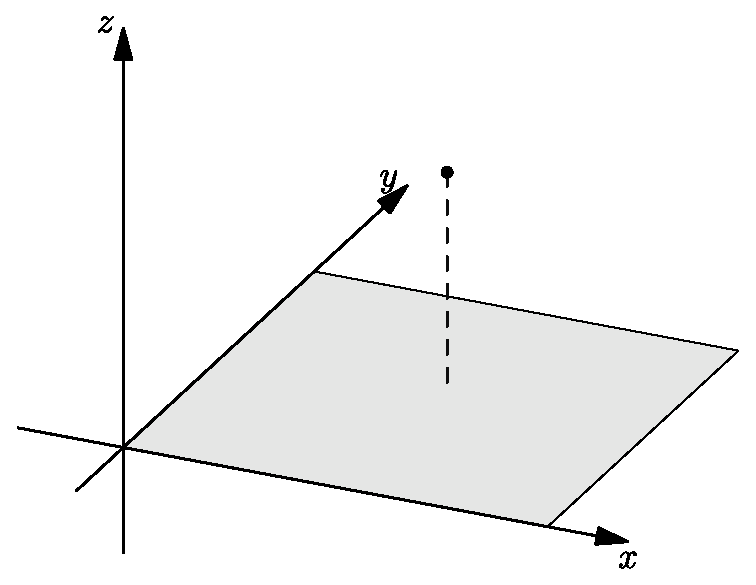
\includegraphics[width=300pt]{Figures/PlanetoDot}\\
    Point to Plane in $\bbr^3$
\end{center}

So if we could just find the point in the plane that is directly ``beneath" our point, then we'd be set. Unfortunately, that's actually really really hard. Fortunately, we don't have to do that.

\begin{exercise}{Point to Plane}
Lets let our plane be the plane $z=0$. Note that this is literally the $xy$-plane. Let's let our point be $(2,1,3)$. Even though it's not hard here to figure out what the point directly below $(2,1,3)$ is, we're gonna assume that we can't. So instead, let's pick a random point on that plane. Like $(4,2,0)$.
\begin{center}
    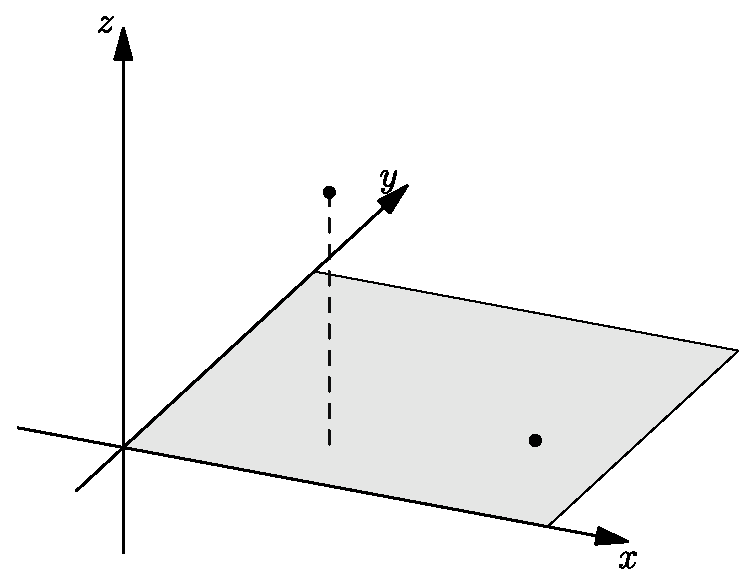
\includegraphics[width=300pt]{Figures/pointplaneex1}\\$(2,1,3)$ and $(4,2,0)$.
\end{center}
\vspace{1em}
\begin{enumerate}
\item Find the vector that goes from $(4,2,0)$ to $(2,1,3)$. Call that vector $\vcv$.
\vspace{1em}
\end{enumerate}
Well, why would we find that vector? It's certainly not the shortest distance between our point and our plane. But if we look at that vector between our two points, you may notice something.
\vspace{1em}
\begin{center}
    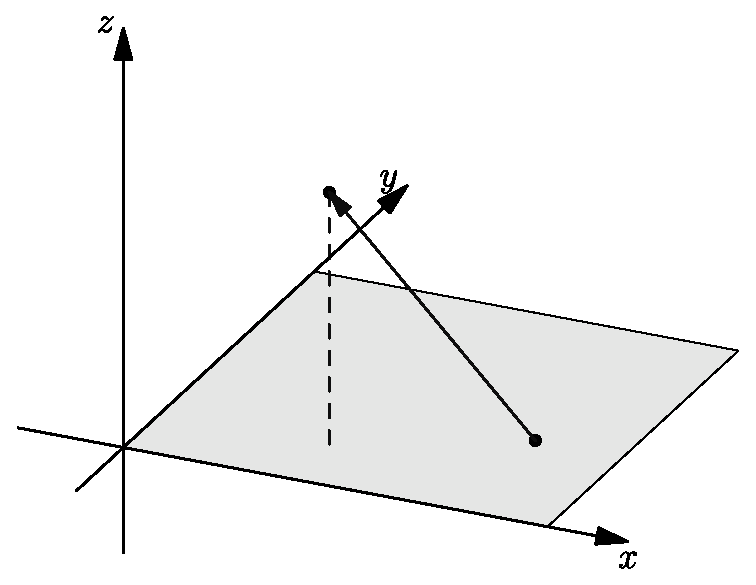
\includegraphics[width=300pt]{Figures/pointplaneex2}\\\href{https://www.geogebra.org/3d/kdsbfgck}{The vector from $(4,2,0)$ to $(2,1,3)$ (Geogebra Link).}
\end{center}
\vspace{1em}
While the length of $\vcv$ is not the distance we are looking for, if we were to find the component of $\vcv$ in the direction perpendicular to our plane, that would, in fact, be the right length. And that's \textit{exactly} what our vector projection is.
\vspace{1em}
\begin{enumerate}
\item[2.] Find $\vcn$, the normal vector for our plane $z=0$.
\vspace{1em}
\item[3.] Find $\proj{\vcv}{\vcn}$, the projection of $\vcv$ onto $\vcn$, and the distance between our point and our plane.
\vspace{1em}
\item[4.] Take the magnitude of the projection you just found. That is, find $|| \proj{\vcv}{\vcn}||$.
\end{enumerate}
\end{exercise}

\begin{claim}{Point to Plane Algorithm}
To find the distance between a point $P$ and a plane:
\vspace{1em}
\begin{enumerate}
\item Pick an arbitrary point, $Q$, on the plane.
\vspace{1em}
\item Find the vector difference between $P$ and $Q$, call that $\vcv$.
\vspace{1em}
\item Find the normal vector for your plane, call that $\vcn$.
\vspace{1em}
\item Find $\proj{\vcv}{\vcn}$, or the projection of $\vcv$ onto $\vcn$.
\vspace{1em}
\item Find $||\proj{\vcv}{\vcn}|| $. This is the distance required.
\end{enumerate}
\end{claim}

So let's now look at the distance between two planes! First, note that if two planes intersect, then they share a point, so the distance between the two planes must be zero. The only way for planes to not intersect is if they are \textit{parallel}. 

\begin{center}
    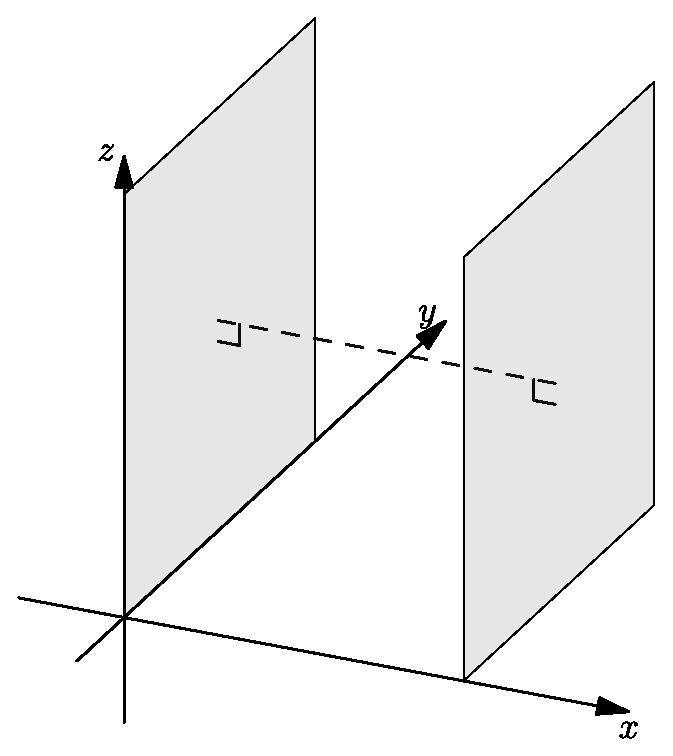
\includegraphics[width=300pt]{Figures/PlanetoPlane}\\
    Parallel Planes in $\bbr^3$
\end{center}

\begin{claim}{Plane to Plane Algorithm}
To find the distance between two planes:
\vspace{1em}
\begin{enumerate}
\item Pick an arbitrary point, $P$ on one of your planes.
\vspace{1em}
\item Execute the Point to Plane algorithm with the chosen $P$ and the other plane.
\end{enumerate}
\end{claim}

\begin{exercise}{Plane to Plane}
Find the distances between the following planes.
\vspace{1em}
\begin{enumerate}
\item Find the distance between \href{https://www.geogebra.org/3d/gn8etvbp}{$2x-y+z=2$ and $2x-y+z=-1$. (Geogebra Link)}
\vspace{1em}
\item Find the distance between \href{https://www.geogebra.org/3d/ekksyyew}{$5x-2y+z=6$ and $5x-2y+z=-3$. (Geogebra Link)}
\end{enumerate}
\end{exercise}

Similarly, the distance between a line and a plane also quickly reduces. If the line intersects the plane, then the distance is 0, but if the line is parallel to the plane, then you pick any point on the line and then use the point to plane algorithm.

\begin{claim}{Line to Plane Algorithm}
To find the distance between a line and a plane:
\vspace{1em}
\begin{enumerate}
\item Pick an arbitrary point, $P$ on your line.
\vspace{1em}
\item Execute the Point to Plane algorithm with the chosen $P$ and the plane.
\end{enumerate}
\end{claim}

\begin{exercise}{Line to Plane}
Find the distances between the following Lines and Planes.
\vspace{1em}
\begin{enumerate}
\item Find the distance between \href{https://www.geogebra.org/3d/guykkgyr}{$2x+y-z=3$ and $\dfrac{x}{2}=\dfrac{y-1}{2}=\dfrac{z}{6}$. (Geogebra Link)}
\vspace{1em}
\item Find the distance between $2x+y-z=3$ and $\dfrac{x}{2}=\dfrac{y-1}{4}=\dfrac{z}{6}$. Hint: is this line parallel to the plane? Check by taking the dot product of the normal vector of the plane and the direction vector of the line.
\end{enumerate}
\end{exercise}
\subsection{Distance to Lines}

Next up is the distance between points and lines. The shortest distance between a point and a line in $\bbr^3$ should certainly be along the path perpendicular to the line, but unfortunately we don't have a great way to generate the direction vector between the line and the point. So we need to do something a little different. 

\begin{claim}{Point to Line}
Consider a line $L$ and a point $P$ such that $P$ does not lie on $L$ (if $P$ lies on $L$ then the distance is zero). Let $L$ have a direction vector of $\vcd$. Then we can draw a line segment from $P$ to $L$ such that that line segment is perpendicular to $L$.
\vspace{1em}
\begin{center}
\begin{tikzpicture}
%	\draw[->, color=red,line width=0.5mm](0,0)--(5,3);
	\draw[<->,line width=0.5mm](-4,0)--(8,0);
%	\draw[->, color=purple,line width=0.7mm](0,0)--(5,0);
	\draw[dashed, line width=0.5mm](5,3)--(5,0);
	\draw[](5,0.3)--(4.7,0.3)--(4.7,0);
	\node at (5,3) {$\bullet$};
	\node at (5.5,3.5) {$P$};
%	\node[color=red] at (2.5,2) {$\vcw$};
	\node at (-0.5,0.5) {$L$};
%	\node[color=purple] at (3,0.5) {$\proj{\vcw}{\vcv}$};
\end{tikzpicture}
\end{center}
\vspace{1em}
Call the point where this perpendicular line segment intersects the line $R$, and then pick an arbitrary point $Q$ on $L$. These three points form the right triangle $\triangle PQR$. Call $\angle PQR=\theta$.
\vspace{1em}
\begin{center}
\begin{tikzpicture}
%	\draw[->, color=red,line width=0.5mm](0,0)--(5,3);
	\draw[<->,line width=0.5mm](-4,0)--(8,0);
%	\draw[->, color=purple,line width=0.7mm](0,0)--(5,0);
	\draw[dashed, line width=0.5mm](5,3)--(5,0);
	\draw[](5,0.3)--(4.7,0.3)--(4.7,0);
	\node at (5,3) {$\bullet$};
	\node at (5.5,3.5) {$P$};
%	\node[color=red] at (2.5,2) {$\vcw$};
	\node at (-1.5,0.5) {$L$};
	\node at (0,0) {$\bullet$};
	\node at (0,-0.5) {$Q$};
	\node at (5,0) {$\bullet$};
	\node at (5,-0.5) {$R$};
	\draw [line width=0.5mm](0,0)--(5,3);
	\draw (0.5,0) arc (0:30:0.5);
	\node at (0.8,0.25) {$\theta$};
%	\node[color=purple] at (3,0.5) {$\proj{\vcw}{\vcv}$};
\end{tikzpicture}
\end{center}
\vspace{1em}
By SOH-CAH-TOA, we know that $$\frac{||\overline{PR}||}{||\overline{PQ}||}=\sin\theta.$$
Also, $||\overline{PR}||$ is the distance we are trying to find, while we can find $||\overline{PQ}||$ by taking the vector difference of the vectors that represent $P$ and $Q$. So we get that the distance between our point and our line can be found using $$d=||\vcp-\vcq||\sin\theta .$$
Finally, we invoke the cross product formula from Theorem 1.4.5, noting that $\theta$ is the angle between $\vcp-\vcq$ and $\vcd$, so:
\begin{align*}
||(\vcp-\vcq)\times\vcd||=&||\vcp-\vcq||\cdot ||\vcd||\sin\theta\\
\frac{||(\vcp-\vcq)\times\vcd||}{||\vcp-\vcq||\cdot ||\vcd||}=&\sin\theta.
\end{align*}
Then by substitution:
\begin{align*}
d=&||\vcp-\vcq||\sin\theta\\
=&||\vcp-\vcq||\frac{||(\vcp-\vcq)\times\vcd||}{||\vcp-\vcq||\cdot ||\vcd||}\\
d=&\frac{||(\vcp-\vcq)\times\vcd||}{ ||\vcd||}
\end{align*}
\end{claim}

\begin{claim}{Point to Line Algorithm}
\begin{enumerate}
\item Find the direction vector for your line, call it $\vcd$.
\vspace{1em}
\item Call the point $P$, represented by vector $\vcp$. Then pick an arbitrary point $Q$ on your line, represented by vector $\vcq$.
\vspace{1em}
\item Find the vector between $P$ and $Q$ as the vector difference $\vcp-\vcq$.
\vspace{1em}
\item Find your distance $d$ as $$d=\frac{||(\vcp-\vcq)\times\vcd||}{ ||\vcd||}. $$
\end{enumerate}
\end{claim}

\begin{exercise}{Point to Line}
Find the distance between the following points and lines.
\vspace{1em}
\begin{enumerate}
\item \href{https://www.geogebra.org/3d/skreh6sd}{Let $P$ be the point $(2,1,-3)$ and $L(t)=\bmat{1\\-1\\4}t+\bmat{0\\1\\0}.$ (Geogebra Link)}
\vspace{1em}
\item \href{https://www.geogebra.org/3d/sfhumpus}{Let $P$ be the point $(1,1,1)$ and $L$ be the line with symmetric form $\dfrac{x}{2}=y-1=2z+1.$ (Geogebra Link)}
\end{enumerate}
\end{exercise}

Our very last case to deal with is the distance between two lines in $\bbr^3$. This is the most complicated case, because there are actually multiple subcases. As usual, if the lines intersect, then the distance is zero. But we have to treat the case where the two lines are parallel a little differently than the two cases where the lines are \textit{skew} to each other.

\begin{exercise}{Parallel, Skew, or Intersect?}
For the following lines, decide if they are parallel, skew, or intersecting lines.
\vspace{1em}
\begin{enumerate}
\item Let $\vec{L}_1(t)=\bmat{1\\2\\3}t+\bmat{0\\0\\-1}$ and $L_2(t)=\bmat{2\\-3\\-1}t+\bmat{1\\2\\2}$. Hint: Set $\vec{L}_1(t)=\vec{L}_2(s)$. Then solve the system of equations presented by the first two coordinates, then check to see if those values of $s$ and $t$ satisfy the third coordinate!
\vspace{1em}
\item Let $L_1(t)=\bmat{2\\3\\-1}t+\bmat{3\\3\\1}$ and $L_2(t)=\bmat{4\\6\\-2}t+\bmat{1\\0\\0}$.
\vspace{1em}
\item Let $\vec{L}_1$ be the line with symmetric form $x=2y-1=3z+1 $ and $\vec{L}_2$ be the line with symmetric form $x-2=\dfrac{y}{2}=2z.$
\end{enumerate}
\end{exercise}

In the parallel case, both lines are contained in some plane. So then you can just pick a point $P$ along one of the two lines, and then proceed with the point to line plan.
\begin{center}
\begin{tikzpicture}
%	\draw[->, color=red,line width=0.5mm](0,0)--(5,3);
	\draw[<->,line width=0.5mm](-4,0)--(8,0);
	\draw[<->,line width=0.5mm](-4,3)--(8,3);
%	\draw[->, color=purple,line width=0.7mm](0,0)--(5,0);
	\draw[dashed, line width=0.5mm](5,3)--(5,0);
	\draw[](5,0.3)--(4.7,0.3)--(4.7,0);
	\node at (5,3) {$\bullet$};
	\node at (5.5,3.5) {$P$};
%	\node[color=red] at (2.5,2) {$\vcw$};
	\node at (-0.5,0.5) {$L_2$};
	\node at (-0.5,3.5) {$L_1$};
	\node at (0,0) {$\bullet$};
	\node at (0,-0.5) {$Q$};
	\node at (5,0) {$\bullet$};
	\node at (5,-0.5) {$R$};
	\draw [line width=0.5mm](0,0)--(5,3);
	\draw (0.5,0) arc (0:30:0.5);
	\node at (0.8,0.25) {$\theta$};
%	\node[color=purple] at (3,0.5) {$\proj{\vcw}{\vcv}$};
\end{tikzpicture}
\end{center}

\begin{claim}{Line to Line Algorithm (parallel)}
\begin{enumerate}
\item Pick an arbitrary point $P$ on one of your lines and an arbitrary point $Q$ on the other line. Call $\vcd$ the direction vector of one of your lines.
\vspace{1em}
\item Proceed with the point to line algorithm.
\end{enumerate}
\end{claim}

\begin{exercise}{}
Why does it not matter which of the two lines we take $\vcd$ from?
\end{exercise}

\begin{exercise}{Line to Line (parallel)}

Find the distance between the following lines.
\vspace{1em}
\begin{enumerate}
\item \href{https://www.geogebra.org/3d/h4zqcru5}{Let $L_1(t)=\bmat{2\\3\\-1}t+\bmat{3\\3\\1}$ and $L_2(t)=\bmat{4\\6\\-2}t+\bmat{1\\0\\0}$. (Geogebra Link)}
\vspace{1em}
\item \href{https://www.geogebra.org/3d/zzu9vwnf}{Let $L_1$ be the line with symmetric form $x=2y-1=\dfrac{z}{2} $ and $L_2$ be the line with symmetric form $x+1=2y=\dfrac{z+4}{2}.$ (Geogebra Link)}
\end{enumerate}
\end{exercise}

Lastly, we consider the case where we have two lines that are \textit{skew} to each other. That is, they are not parallel but do not intersect.

\begin{exercise}{Skew Lines and Parallel Planes}
Consider two lines, $L_1$, which has parametric form $$L_1(t)=\bmat{t\\t\\0}$$ and $L_2$ which has parametric form $$L_2(t)=\bmat{t\\-t\\2}. $$
\begin{enumerate}
\item Find $\vcd_1$, the direction vector for $L_1$ and $\vcd_2$, the direction vector for $L_2$.
\vspace{1em}
\item How can we tell that $L_1$, $L_2$ are not parallel?
\vspace{1em}
\item Pull up the graph of these two lines on \href{https://www.geogebra.org/3d/dwvfymu7}{Geogebra 3D}.
\vspace{1em}
\item Graph the two parallel planes, $z=0$ and $z=2$ in that same Geogebra 3d window. Verify that your two lines are contained in these two planes and the two planes are parallel.
\vspace{1em}
\item Use $\vcd_1$, $\vcd_2$ and the point $(0,0,0)$ to generate the parametric form of a plane. Then convert that parametric plane to standard form and verify that it is, in fact, the plane $z=0$.
\vspace{1em}
\item Use $\vcd_1$, $\vcd_2$ and the point $(0,0,2)$ to generate the parametric form of a plane. Then convert that parametric plane to standard form and verify that it is, in fact, the plane $z=2$.
\end{enumerate}
\end{exercise}

The idea contained in the previous exercise generalizes. In fact, given two skew lines, we can always generate two parallel planes, one containing each line, which reduces us to the plane to plane case. We can algorithmically kinda mash some steps together to get us straight to good old point to plane.

\begin{claim}{Line to Line Algorithm (skew)}
\begin{enumerate}
\item Call your two lines $L_1$, $L_2$. Find the two direction vectors, $\vcd_1$, $\vcd_2$.
\vspace{1em}
\item Find a point $Q$ on $L_1$. Then generate the plane that contains $L_1$ that is parallel to $L_2$ by using the two direction vectors $\vcd_1$, $\vcd_2$ and containing $Q$.
\vspace{1em}
\item Pick an arbitrary point $P$ on $L_2$, then proceed with point to plane algorithm.
\end{enumerate}
\end{claim}

\begin{exercise}{Line to Line (skew)}
Find the distance between the following lines.
\vspace{1em}
\begin{enumerate}
\item \href{https://www.geogebra.org/3d/js6pygd7}{Let $\vec{L}_1(t)=\bmat{1\\1\\-1}t+\bmat{2\\4\\1}$ and $\vec{L}_2(t)=\bmat{-2\\1\\3}t+\bmat{1\\1\\3}$. (Geogebra Link)}
\vspace{1em}
\item \href{https://www.geogebra.org/3d/y349fgsf}{Let $\vec{L}_1$ be the line with symmetric form $x=2y-1=3z+1 $ and $L_2$ be the line with symmetric form  $x-2=\dfrac{y}{2}=2z.$(Geogebra Link)}
\end{enumerate}
\end{exercise}
\renewcommand\thesubsection{\thesection.\Alph{subsection}}
\setcounter{subsection}{18}
\subsection{Points, Lines and Planes Summary}
\begin{definition}{Forms of a Plane}
\begin{itemize}
\item \textbf{Standard Form:} $$ax+by+cz=d\text{ where }\bmat{a\\b\\c}\text{ is the normal vector.} $$
\item \textbf{Parametric Form:} Let $\vcr_0$ lie in the plane and $\vcd_1$ and $\vcd_2$ be independent vectors parallel to the plane. Then the plane can be parameterized as:
$$\vcr(s,t)=\vcr_0+\vcd_1 s+\vcd_2 t.$$
\item \textbf{Vector-Dot Product Form:} Let $$\vcr_0=\bmat{x_0\\y_0\\z_0}$$ lie in the plane and $$\vcn=\bmat{a\\b\\c} $$ be normal to the plane. Then we can write the plane as
\begin{align*}
(\vcx-\vcr_0)\bullet \vcn=&0\\
\bmat{x-x_0\\y-y_0\\z-z_0}\bullet\bmat{a\\b\\c}=&0\\
a(x-x_0)+b(y-y_0)+c(z-z_0)=&0.
\end{align*}
\end{itemize}
\end{definition}

\begin{definition}{Forms of a Line}
Let $\vcd=\bmat{a\\b\\c}$ be the direction vector and $\vcx=\bmat{x_0\\y_0\\z_0}$ be a point the line passes through.
\begin{itemize}
\item \textbf{Parametric Form:} The line that passes through $\vcx$ with direction $\vcd$ is given in parametric form as $$\vcr(t)=\vcd\cdot t+\vcx. $$
\item \textbf{Symmetric Form:} The line that passes through $\vcx$ with direction $\vcd$ can be described using the symmetric form equation $$\vcd=\bmat{a\\b\\c} $$ is $$\frac{x-x_0}{a}=\frac{y-y_0}{b}=\frac{z-z_0}{c}.$$
\item \textbf{``Standard" Form:} The line that passes through $\vcx$ with direction $\vcd$ can also be given by the intersection of two planes with normal vectors $\vcn_1$ and $\vcn_2$ where $\vcn_1\times\vcn_2=\pm\vcd$ and $\vcx$ lies in both planes.
\end{itemize}
\end{definition}

\begin{definition}{Distance from Point, Line or Plane to Plane}
\begin{itemize}
\item To find the distance between a point $P$ and a plane, you should pick some point $Q$ in the plane. Then take the vector between $P$ and $Q$, and project that vector onto the normal vector of the plane, that is the distance $d$ is found as $$d=\proj{\vcp-\vcq}{\vcn} $$ where $\vcp$ is the vector that represents the point $P$ and $\vcq$ is the vector that represents the point $Q$.

\vspace{1em}

\item To find the distance between a line and a plane, check to see if the line intersects the plane. If the direction of the line and normal vector to the plane are perpendicular, then the line does not intersect the plane unless it coincides with the plane. Otherwise, they intersect and the distance is zero. If they do not intersect, then pick any point $P$ on the line and find the distance between $P$ and the plane.

\vspace{1em}

\item To find the distance between two planes, first check to see if the planes are parallel by checking if the normal vectors are parallel. If they are not parallel, then the distance between the two is zero. If they \textit{are} parallel, then pick any point $P$ on one of the two planes and find the distance between $P$ and the other plane.
\end{itemize}
\end{definition}

\begin{definition}{Point to Line}

To find the distance between a point $P$ and a line, pick some point $Q$ on the line, then use the formula $$d=\frac{||(\vcp-\vcq)\times\vcd||}{||\vcd||} $$ where $\vcp$ is the vector the represents the point $P$, $\vcq$ is the vector that represents the point $Q$, and $\vcd$ is the direction vector of the line.
\end{definition}

\begin{definition}{Line to Line}
\begin{itemize}
\item If the two lines are \textit{parallel} to each other, pick a point $P$ on one of the two lines, then proceed to use point to line to find the distance between $P$ and the other line.

\vspace{1em}

\item If the two lines are \textit{skew} to each other, then use the direction vectors of the two lines and a point $Q$ on one of the two lines to generate a plane that is parallel to both lines and contains one of the lines. Then proceed with finding the distance between the other line and your new plane.
\end{itemize}
\end{definition}

\subsubsection*{Companion Videos by Ken Monks}
\begin{itemize}
\item \href{https://www.youtube.com/watch?v=ZVJzzVEpwsQ}{Planes in 3D.}
\item \href{https://www.youtube.com/watch?v=H0yZECa1HZA}{Lines in 3D.}
\item \href{https://www.youtube.com/watch?v=xxpIPthhOUg}{Distance between Points, Lines and Planes in 3D, Part 1.}
\item\href{https://www.youtube.com/watch?v=LIsp59EGbnk}{Distance between Points, Lines and Planes in 3D, Part 2.}
\end{itemize}

\renewcommand\thesubsection{\thesection.\arabic{subsection}}
\renewcommand\thesubsection{\thesection.\Alph{subsection}}
\setcounter{subsection}{17}
\subsection{Points, Lines and Planes Homework and Miscellaneous Practice}

\begin{exercise}{Standard to Parametric, Lines}
Consider the two planes $2x+y-z=3$ and $x-2y+z=1$. Give the equation of the line that is the intersection of these two planes in parametric form.
\end{exercise}

\begin{exercise}{Symmetric Form of a Line}
Consider the line that passes through the point $(-2,1,3)$ with direction vector $\vcd=\vci+\frac{1}{2}\vcj-2\vck$. Give the equation of this line in symmetric form.
\end{exercise}

\begin{exercise}{Standard Form of a Line}
Consider the line that passes through the point $(-2,1,3)$ with direction vector $\vcd=\vci+\frac{1}{2}\vcj-2\vck$. Find the equation of the two planes who's intersection is this line.
\end{exercise}

\begin{exercise}{Standard Form of a Plane}
Find the equation in standard form of a plane that contains the point $(1,0,3)$ and is parallel to the vectors $\vcd_1=\bmat{2,1,-1}$ and $\vcd_2=\bmat{1,2,3}$.
\end{exercise}

\begin{exercise}{Vector-Dot Product Form of a Plane}
Find the equation in vector-dot product form of a plane that contains the point $(1,0,3)$ and is parallel to the vectors $\vcd_1=\bmat{2,1,-1}$ and $\vcd_2=\bmat{1,2,3}$.
\end{exercise}

\begin{exercise}{Standard to Parametric, Planes}
Find the equation in parametric form of a plane $3x-y+z=5$.
\end{exercise}

\begin{exercise}{Point to Point}
Find the distance between the point $(1,2,3)$ and $(-1,5,-3)$.
\end{exercise}

\begin{exercise}{Point to Plane}
Find the distance between the point $(1,3,2)$ and the plane $-x+y-2z=3$.
\end{exercise}

\begin{exercise}{Plane to Plane}
Find the distance between the two planes $x+y-z=3$ and $2x+2y-2z=5$.
\end{exercise}

\begin{exercise}{Line to Plane}
Find the distance between the plane $-x+y+z=2$ and the line $\vec{L}(t)=\bmat{t+1\\-t\\2t}$.
\end{exercise}

\begin{exercise}{Point to Line}
Find the distance between the point $(1,2,4)$ and the line $\vec{L}(t)=\bmat{t+1\\-t\\2t}$.
\end{exercise}

\begin{exercise}{Line to Line (parallel)}
Find the distance between the two lines, $\vec{L}_1(t)=\bmat{t+1\\-t\\2t}$ and $\vec{L}_2(t)=\bmat{-t\\t+2\\-2t+7}$.
\end{exercise}

\begin{exercise}{Line to Line (skew)}
Find the distance between the two lines, $\vec{L}_1(t)=\bmat{2t+1\\-t+1\\t}$ and $\vec{L}_2(t)=\bmat{3t+2\\-5t+1\\2t-1}$.
\end{exercise}
\renewcommand\thesubsection{\thesection.\arabic{subsection}}

\section{Parametric Curves}
\hypertarget{paraderiv}{\subsection{Parametric Functions and their Derivatives}}

Our first foray into multivariate calculus is functions with multiple outputs. The best way to scale this out is by using a \textbf{parametric} or \textbf{vector valued} function, which you should be mildly familiar with from Calculus II. But for the sake of completion:

\begin{definition}{Parametric Functions}
A \textbf{parametric function} or \textbf{vector-valued function} is a function $r:\bbr\to\bbr^n$. We usually write a parametric function as an $n$-dimensional vector of functions, typically all with a placeholder input variable of $t$. That is: $$\vcr(t)=\bmat{x_1(t)\\x_2(t)\\ \vdots \\ x_n(t)}.$$

\end{definition}

\begin{definition}{Vector Function Derivative}
We define the derivative of a vector-valued function componentwise. That is, if $$\vcr(t)=\bmat{x_1(t)\\x_2(t)\\ \vdots \\ x_n(t)},$$
then
\begin{align*}
\vcr\hspace{0.2em}'(t)=&\frac{d}{dt}\big(\vcr(t)\big)\\
=&\bmat{\frac{d}{dt}\big(x_1(t)\big)\\\frac{d}{dt}\big(x_2(t)\big)\\ \vdots \\ \frac{d}{dt}\big(x_n(t)\big)}\\
=&\bmat{x_1'(t)\\x_2'(t)\\ \vdots \\ x_n'(t)}.
\end{align*}
\end{definition}

As with the single variable derivative, this vector derivative follows some quite nice properties. In particular, linearity holds.

\begin{claim}{Linearity of Vector Derivative}
Let $\vec{r_1}(t)$ and $\vec{r_2}(t)$ be $n$ dimensional vector valued functions and let $c_1,c_2\in\bbr$. Then $$\left(c_1\vec{r_1}(t)+c_2 \vec{r_2}(t)\right)'=c_1\vec{r_1}'(t)+c_2\vec{r_2}'(t).$$ 
\end{claim}

We also get three distinct but almost identical product rules for our three distinct products, scalar, dot and cross.

\begin{claim}{Scalar Product Rule}
Let $\vcr(t)$ be a $n$-dimensional vector function and $f(t)$ be a scalar function. Then $$\big(f(t)\vcr(t)\big)'=f(t)\vcr\hspace{0.2em}'(t)+f'(t)\vcr(t).$$
\end{claim}

\begin{claim}{Dot Product Rule}
Let $\vcr_1(t)$ and $\vcr_2(t)$ be $n$-dimensional vector functions. Then $$\big(\vcr_1(t)\bullet\vcr_2(t)\big)'=\vcr_1(t)\bullet\vcr_2\hspace{0.2em}'(t)+\vcr_1\hspace{0.2em}'(t)\bullet\vcr_2(t).$$
\end{claim}

\begin{claim}{Cross Product Rule}
Let $\vcr_1(t)$ and $\vcr_2(t)$ be $3$-dimensional vector functions. Then $$\big(\vcr_1(t)\times\vcr_2(t)\big)'=\vcr_1(t)\times\vcr_2\hspace{0.2em}'(t)+\vcr_1\hspace{0.2em}'(t)\times\vcr_2(t).$$
\end{claim}

\begin{exercise}{Scalar Quotient Rule?}
While it doesn't make any sense to divide a scalar by a vector or to divide two vectors using either of our vector products, we can certainly divide a vector by a scalar. Prove the scalar quotient rule. That is, let $$\vcr(t)=\bmat{x_1(t)\\x_2(t)\\ \vdots\\x_n(t)},$$ and $f(t)$ be a scalar function. Prove that $$\left(\frac{\vcr(t)}{f(t)}\right)'=\frac{f(t)\vcr\hspace{0.2em}'(t)-\vcr(t)f'(t)}{\left(f(t)\right)^2}. $$ Hint: There are two primary approaches here. You can rewrite the division as multiplication by the reciprocal, then proceed to use the scalar product rule and the traditional chain rule, or you could use the traditional quotient rule and component wise differentiation!
\end{exercise}

\begin{exercise}{Derivatives? I remember \textit{those}}
Find the following derivatives:
\begin{enumerate}
\item Find $\vcr\hspace{0.2em}'(t)$ where $\vcr(t)=\bmat{t^2+2\\ \sin(t)\\ \tan(t)}.$
\vspace{1em}
\item Find $\vcr\hspace{0.2em}'(t)$ where $\vcr(t)=\bmat{\cos(t^2-4)\\ e^t\ln(t)\\ \arctan(t)}.$
\vspace{1em}
\item Find $\dfrac{d}{dt}\left(\bmat{\frac{t}{t+3}\\ t^2-4\\t+6}\bullet\bmat{t+3\\ \frac{1}{t-2}\\ \sin(t)}\right).$
\vspace{1em}
\item Find $\dfrac{d}{dt}\left(\bmat{t\\3t\\ \sin(t)}\times\bmat{\cos(t)\\3\\e^t}\right).$
\vspace{1em}
\end{enumerate}
\end{exercise}
\subsection{Position, Velocity, Acceleration, Take 2}
Here we have some particular terms we wish to define to carefully define our generalization of the idea of the derivative as the \textit{slope of the tangent line}. Definition vomit ahoy!

\begin{definition}{Position}
If we imagine our parametric curve represents an object's motion in space, then the \textbf{position} function is just the parametric curve $\vcr(t)$ where $$ \vcr(t)=\bmat{x(t)\\y(t)\\z(t)}$$ for some functions $x(t)$, $y(t)$, $z(t)$.
\end{definition}

\begin{definition}{Velocity}
Then velocity, $\vcv(t)$ is just the derivative of position with respect to time. That is, $\vcv(t)=\vcr\hspace{0.2em}'(t)$ or $$\vcv(t)=\bmat{x'(t)\\y'(t)\\z'(t)}.$$
\end{definition}

\begin{definition}{Speed}
You may have heard the phrase ``velocity is a vector and speed is a scalar". Speed is just the scalar version of velocity-- where velocity has a direction, speed is just the magnitue of the velocity vector. That is, $v=||\vcv(t)||=||\vcr\hspace{0.2em}'(t)||.$
\end{definition}

\begin{definition}{Acceleration}
Acceleration is the derivative of velocity with respect to time. That is, $\vca(t)=\vcv\vprime(t)=\vcr\vprime'(t)$.
\end{definition}

Rather than just a slope, however, in order to describe the direction of a function at a given point we need a \textbf{tangent vector}. We also generally wish to just describe the \textit{direction} of the change of the function rather than the \textit{magnitude} of the change. Because of this, we desire that our tangent vector be a unit vector. So then we get the following definition.

\begin{definition}{Tangent Vector}
The \textbf{tangent vector} for a function, $\vcT(t)$ is the unit vector parallel to the velocity vector. That is, $$\vcT(t)=\frac{\vcv(t)}{v}=\frac{\vcv(t)}{||\vcv(t)||}=\frac{\vcr\vprime(t)}{||\vcr\vprime{t}||}. $$
\end{definition}

Note that this yields the equation of a tangent line in 3-d.

\begin{definition}{Tangent Line}
Let $\vcr(t)$ be a vector function in $n$-dimensional space and let $\vcv(t)$ be the $\vcr\vprime(t)$. Then the equation of the line tangent to $\vcr(t)$ at $t=a$ in parametric form is $$\vcl(t)=\vcv(a)\cdot t+\vcr(a). $$
\end{definition}

We get a couple of followup definitions out of this. In particular, since these functions are often changing directions, we get an idea of \textbf{angular velocity}.

\begin{definition}{Angular Velocity}
The \textbf{angular velocity} for a function $\vcr(t)$ is the change in the tangent vector. That is, $$\vomega(t)=\vcT\vprime(t). $$
\end{definition}

\begin{definition}{Angular Speed}
Just like velocity to speed, angular speed is just the magnitude of angular velocity. That is, $$\omega(t)=||\vomega(t)||=||\vcT\vprime(t)||. $$
\end{definition}

This angular velocity idea lets us define the \textbf{normal vector} for a function. Where the tangent vector indicates the direction of motion of the function, the normal vector indicates the direction of change for the \textit{tangent vector itself}.

\begin{definition}{Normal Vector}
The \textbf{normal vector} to a function $\vcr(t)$ is the unit vector parallel to the angular velocity. That is, $$\vcN(t)=\frac{\vomega(t)}{\omega(t)}=\frac{\vcT\vprime(t)}{||\vcT\vprime(t)||}. $$
\end{definition}

\begin{example}{Tangents and Normals}
Let's consider the position function $$\vcr(t)=\bmat{\sin(t)\\ \cos(t)\\t}. $$
This generates a helix.
\begin{center}
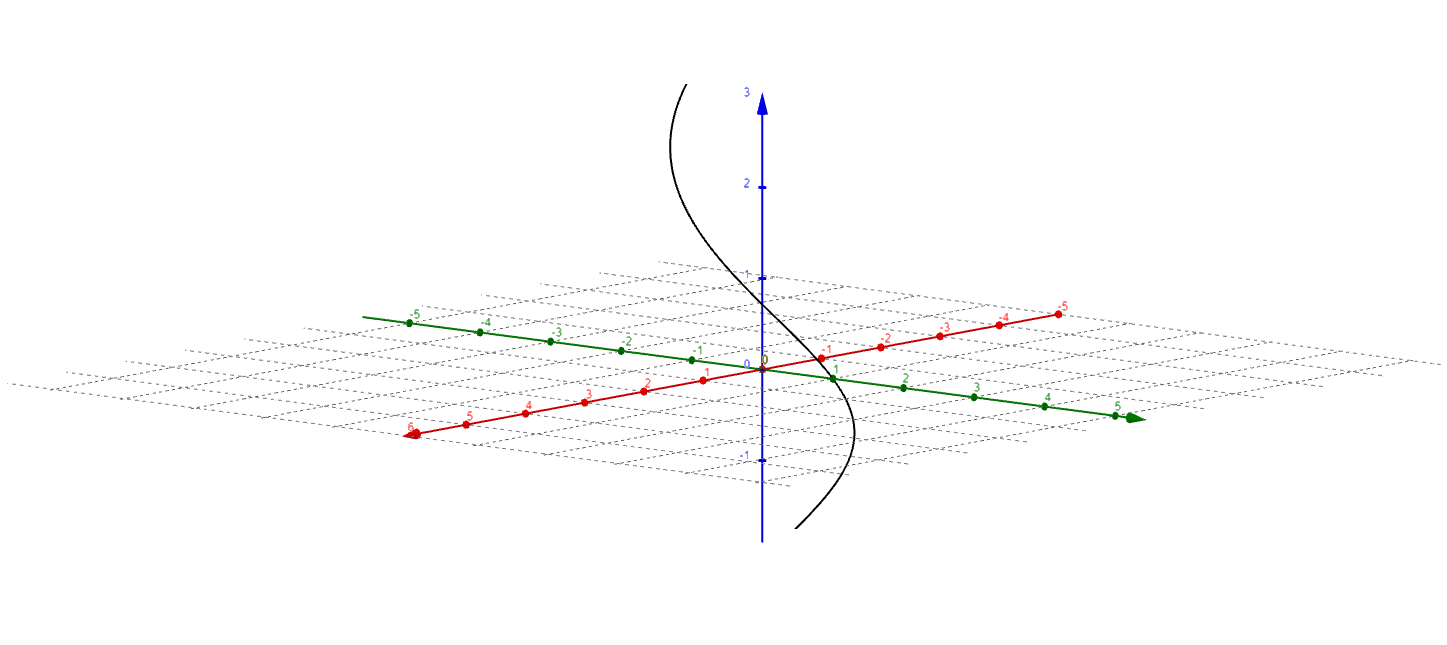
\includegraphics[scale=0.3]{Figures/tangentnormalex}
\\
Graph of $\vcr(t)$.
\end{center}
\vspace{1em}
Finding the velocity of object is a matter of taking the derivative component-wise:
$$\vcv(t)=\bmat{\cos(t)\\-\sin(t)\\1}. $$
Then we can find $v$, the speed:
\begin{align*}
v=&||\vcv||\\
=&\sqrt{\cos^2(t)+(-\sin(t))^2+1^2}\\
=&\sqrt{\cos^2(t)+\sin^2(t)+1}\\
=&\sqrt{2}.
\end{align*}
Then we can find the tangent vector $$\vcT(t)=\frac{\vcv}{v}=\bmat{\frac{\cos t}{\sqrt2}\\ -\frac{\sin t}{\sqrt2}\\ \frac{1}{\sqrt{2}}}.$$
From there, to find the normal vector we differentiate for the angular velocity, then normalize.
$$\vomega(t)=\vcT\vprime(t)=\bmat{\frac{-\sin t}{\sqrt{2}}\\ \frac{-\cos t}{\sqrt{2}}\\ 0}.$$
The angular speed, $||\vcT\vprime(t)||=\frac{1}{\sqrt{2}}$, so our normal vector is $$\vcN(t)=\frac{\vomega}{\omega}=\bmat{-\sin t\\ -\cos t\\ 0}. $$
You can visit this \href{https://www.geogebra.org/3d/rfrp5b9b}{Geogebra link} to view the function, along with it's tangent and normal vector (tangent in blue, normal in red). You can vary the value of $a$ to move the tangent/normal vectors along the curve and see how they change along the path.
\end{example}

\begin{exercise}{Tangents and Normals}\label{tandn}
Let $$\vcr(t)=\bmat{t\\2\sin(t)\\2\cos(t)} .$$
\begin{enumerate}
\item Find the tangent vector $\vcT(t)$.
\vspace{1em}
\item Find the equation of the line tangent $\vcr(t)$ at $t=\frac{\pi}{3}$ in parametric form. (your direction vector can just be the velocity vector to the function at the given point!) \href{https://www.geogebra.org/3d/cngzwkaw}{Geogebra Link}
\vspace{1em}
\item Find the normal vector $\vcN(t)$.
\vspace{1em}
\item Of occasional use is the \textbf{binormal vector}, which is the cross product of the tangent and normal vectors. Compute the binormal vector for $r(t)$.
\end{enumerate}
\end{exercise}
\subsection{Curvature, Osculating Circles and Evolutes}
The concept of curvature is related to to the ideas from the previous section. Curvature is essentially the ratio of angular speed to linear speed.

\begin{definition}{Curvature}
Curvature can be found as the ratio $$\kappa(t)=\frac{\omega(t)}{v(t)}=\frac{||\vcT\vprime(t)||}{||\vcr\vprime(t)||}.$$
The reciprocal of curvature is the \textbf{radius of curvature}, written as $R(t)=\frac{1}{\kappa(t)}.$

\vspace{1em}
Note also an alternative form to compute curvature:
$$\kappa(t)=\frac{||\vcv(t)\times\vca(t)||}{||\vcv(t) ||^3}= \frac{||\vcr\vprime(t)\times\vcr\vprime'(t)||}{||\vcr\vprime(t) ||^3}. $$
\end{definition}

For a given point along the curve, the radius of curvature is the radius of the \textbf{osculating circle} at that point. If the tangent line is the best linear approximation of a curve at a given point, the osculating circle is the best circular approximation of a curve at a given point! The centers of the osculating circles for a given function have a specific name also.

\begin{definition}{Evolute}
The \textbf{evolute}, $\vcE(t)$ of a curve, $\vcr(t)$ is the set of centers of the osculating circles for the curve. That is, if we let $a\in\bbr$, $\vcr(a)$ is a point on $\vcr(t)$, and $\vcE(a)$ is the center of the osculating circle to $\vcr(t)$ at $\vcr(a)$. We can compute the evolute as
$$\vcE(t)=\vcr(t)+\frac{1}{\kappa(t)}\vcN(t).$$
\end{definition}

\begin{example}{Evolutes, Osculating Circles and Curvature}
Lets consider the helix from the prior example, $$\vcr(t)=\bmat{\sin t\\ \cos t\\ t}. $$ We'll begin by computing the curvature. Fortunately for us, our curvature will be constant in the helix, which makes our lives \textit{quite} a bit easier. Recall that the speed was $v=\sqrt{2}$ and the angular speed was $\omega=\frac{1}{\sqrt{2}}$. Then we can compute $$\kappa=\frac{\omega}{v}=\frac{\frac{1}{\sqrt{2}}}{\sqrt{2}}=\frac{1}{2}. $$
Then our radius of curvature will be the reciprocal, or $2$. Lastly, we can use curvature to compute the evolute.
\begin{align*}
\vcE(t)=&\vcr(t)+\frac{1}{\kappa(t)}\vcN(t)\\
=&\bmat{\sin t\\ \cos t\\ t}+2\bmat{-\sin t\\ -\cos t\\ 0}\\
\vcE(t)=&\bmat{-\sin t\\ -\cos t\\ t}.
\end{align*}

Again, you can follow this \href{https://www.geogebra.org/3d/fgypvuu4}{Geogebra link} to check out this on a 3d plot. The purple curve is the evolute, and the blue circle represents the osculating circle at the point $r(a)$.
\end{example}

\begin{example}{Osculating Circles with Non-Constant Curvature}
At this \href{https://www.desmos.com/calculator/7leqtbvxck}{Desmos Link} you can see an example of an osculating circle that changes in magnitude based on a curve in 2-d. You can also change the functions $f(x)$ and $g(x)$ to see an example of your own parametric function, $$\vcr(t)=\bmat{f(t)\\g(t)}. $$
\begin{center}
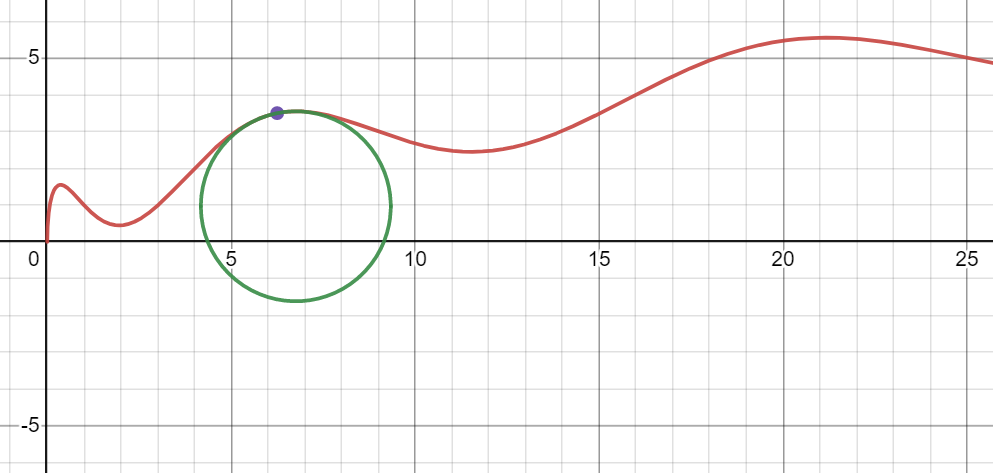
\includegraphics[scale=0.3]{Figures/osculatingcircles}
\end{center}
\end{example}

\begin{exercise}{Curvature and Evolutes}
Let $$\vcr(t)=\bmat{t\\ 2\sin(t)\\ 2\cos(t)}.$$
\vspace{1em}
\begin{enumerate}
\item Find $\vcT(t)$ and $\vcN(t)$, the tangent and normal vectors for $\vcr(t)$.
\vspace{1em}
\item Find $\kappa(t)$, the curvature of $\vcr(t)$.
\vspace{1em}
\item Find $\vcE(t)$, the evolute of $\vcr(t)$.
\end{enumerate}
\end{exercise}

\begin{exercise}{Curvature 2, Electric Boogaloo}
Let $$\vcr(t)=\bmat{t^2\\0\\t}.$$
\vspace{1em}
\begin{enumerate}
\item Find $\kappa(t)$, the curvature of $\vcr(t)$. (hint, it might be easier to calculate this using the second formula for curvature!)
\end{enumerate}
\end{exercise}
\subsection{Integrals and Arc Length}

We define the integral of a vector function in much the same way that we defined the derivative of a vector function:

\begin{definition}{Integral of Vector Function}
The indefinite integral of a vector function with respect to $t$ is done coordinatewise. That is, for $$\vcr(t)=\bmat{x(t)\\y(t)\\z(t)}, $$
$$\int \vcr(t) \ dt=\bmat{\int x(t)\ dt\\ \int y(t)\ dt\\ \int z(t)\ dt}. $$
Similarly, the definite integral is defined:
$$\int_a^b \vcr(t) \ dt=\bmat{\int_a^b x(t)\ dt\\ \int_a^b y(t)\ dt\\ \int_a^b z(t)\ dt}. $$
\end{definition}

This doesn't have a particularly relevant geometric definition, as we're integrating a parametric function. It can kind of best be thought of as an ``accumulation function", where we're accumulating the change in $\vcr(t)$ over some interval of time. It's also just helpful as notation for the antiderivative, i.e. if you're given the velocity function you can integrate to recover the position function, etc.

\begin{exercise}{Antidifferentiating}
Suppose you have a projectile that is moving in 3-d space with velocity function $$\vcv(t)=\bmat{\sin(t)\\t\\t^2},$$ and at time $t=0$ the projectile is at the origin. What is $\vcr(t)$, the position function for this projectile?
\end{exercise}

Something that \textit{does} have relevant geometry is the \textit{arc length}. You may recall the arc length formula from Calculus II for a curve $y=f(x)$ on the $x$-interval $[a,b]$ as:

$$\ell(x)=\int_{a}^{b} \sqrt{1+\left(\tfrac{dy}{dx}\right)^2} \ dx. $$

We also saw a parametric version of this same curve, where $f$ is parameterized via an $x(t)$, $y(t)$:

$$\ell(t)=\int_{a}^{b} \sqrt{\left(\tfrac{dx}{dt}\right)^2+\left(\tfrac{dy}{dt}\right)^2}\ dt. $$

And in fact, given the function $$\vcr(t)=\bmat{x(t)\\y(t)}, $$ this is exactly the integral:
$$\ell(t)=\int_{a}^{b} ||\vcr\vprime(t)|| \ dt. $$

\begin{definition}{Arc Length of a Curve}
Let $\vcr(t)$ be a $n$-dimensional vector valued function. Then the \textbf{arc length} of $\vcr(t)$ between $t=a$ and $t=b$ is $$\ell(t)=\int_{a}^{b} ||\vcr\vprime(t)|| \ dt. $$
\end{definition}

\begin{exercise}{Arc Length of an Helix}
Let $$\vcr(t)=\bmat{\sin t\\ \cos t\\ t}.$$ Find the length of \href{https://www.geogebra.org/3d/a3g6kayf}{this curve (Geogebra Link)} from $t=0$ to $t=2\pi$.
\end{exercise}

\begin{exercise}{Arc Length of a Stretchy Helix}
Let $$\vcr(t)=\bmat{\sin t\\ \cos t\\ \frac{t^2}{2}}.$$ Find the length of \href{https://www.geogebra.org/3d/e34aasz5}{this curve (Geogebra Link)} from $t=0$ to $t=2\pi$.
\end{exercise}
\renewcommand\thesubsection{\thesection.\Alph{subsection}}
\setcounter{subsection}{18}
\subsection{Parametric Curves Summary}

\begin{definition}{Derivative of a Parametric Function}
Let $$\vcr(t)=\bmat{x_1(t)\\x_2(t)\\\vdots\\x_n(t)}.$$ Then $$\vcr\vprime(t)=\bmat{x_1'(t)\\x_2'(t)\\\vdots\\x_n'(t)}. $$ This follows most of the expected rules for derivatives (linearity, product rules for scalar, dot and cross product, quotient rule for scalar quotient, etc.)
\end{definition}

\begin{definition}{Position, Velocity, Acceleration}
Let $\vcr(t)$ define the position of an object in two or three dimensional space. Then $\vcr\vprime(t)=\vcv(t)$, the velocity of the object, and $\vcv\vprime'(t)=\vca(t)$, the acceleration of the object.
\end{definition}

\begin{definition}{Tangent Line}
The parametric equation of the line tangent to $\vcr(t)$ at $t=a$ is $$\vcl(t)=\vcr\vprime(a)t+\vcr(a).$$
\end{definition}

\begin{definition}{Tangent Vector}
The tangent vector, or unit tangent vector, $\vcT(t)$, is the unit vector in the direction of the velocity vector of a function. That is, $$\vcT(t)=\frac{\vcr\vprime(t)}{||\vcr\vprime(t)||}.$$
\end{definition}

\begin{definition}{Angular Velocity}
The angular velocity, $\vomega(t)$ is the change in the tangent vector with respect to time. That is, $$\vomega(t)=\vcT\vprime(t).$$
\end{definition}

\begin{definition}{Normal Vector}
The normal vector, or unit normal vector, $\vcN(t)$ is the unit vector in the direction of the angular velocity of a function. That is, $$\vcN(t)=\frac{\vcT\vprime(t)}{||\vcT\vprime(t)||}. $$
\end{definition}

\begin{definition}{Curvature}
The curvature of a curve, $\kappa(t)$ is the ratio between the angular speed and linear speed of a curve, or $$\kappa(t)=\frac{||\vcT\vprime(t) ||}{||\vcr\vprime(t) ||}. $$ The radius of curvature, $R(t)$ is the reciprocal of the curvature. The radius of curvature is also the radius of the osculating circle, the best circular approximation of a function at a given point.
\end{definition}

\begin{definition}{Alternative Formula for Curvature}
It is often more efficient to compute curvature using the alternative formula $$\kappa(t)=\frac{||\vcr\vprime(t)\times\vcr\vprime'(t) ||}{||\vcr\vprime(t) ||^3}.$$
\end{definition}

\begin{definition}{Evolute}
The evolute of a curve, $\vcE(t)$, is the set of centers of the osculating circles for the curve, given as $$\vcE(t)=\vcr(t)+\frac{1}{\kappa(t)}\vcN(t). $$
\end{definition}

\begin{definition}{Integral of Parametric Function}
Let $$\vcr(t)=\bmat{x_1(t)\\x_2(t)\\\vdots\\x_n(t)}.$$ Then $$\int\vcr(t)\ dt=\bmat{\int x_1(t) \ dt\\\int x_2(t)\ dt\\\vdots\\\int x_n(t)\ dt}. $$
\end{definition}

\begin{definition}{Arc Length of a Curve}
Let $\vcr(t)$ be a $n$-dimensional vector valued function. Then the \textbf{arc length} of $\vcr(t)$ between $t=a$ and $t=b$ is $$\ell(t)=\int_{a}^{b} ||\vcr\vprime(t)|| \ dt. $$
\end{definition}



\renewcommand\thesubsection{\thesection.\arabic{subsection}}
\renewcommand\thesubsection{\thesection.\Alph{subsection}}
\setcounter{subsection}{17}
\subsection{Parametric Curves Homework and Miscellaneous Practice}

\begin{pexercise}{Tangent}%pon
Find the tangent vector $\vcT(t)$ for the vector function $$\vcr(t)=\bmat{t^2+1\\3-t\\t^3}.$$
\end{pexercise}

\begin{pexercise}{Tangent Line}%pon
Give the equation in parametric form of the line that is tangent to $$\vcr(t)=\bmat{\cos(4t)\\ 3\sin(4t)\\ t^3}\text{ at } t=\pi.$$
\end{pexercise}

\begin{exercise}{Tangent and Normal}
Find the tangent vector and normal vector for the function $$\vcr(t)=\bmat{\cos(2t)\\ \sin(2t)\\ 3}. $$
\end{exercise}

\begin{pexercise}{Curvature}%pon
Find the curvature of the function $$\vcr(t)=\bmat{4t\\-t^2\\2t^3}. $$
\end{pexercise}

\begin{pexercise}{Evolute}%pon
Find the evolute of the function $$\vcr(t)=\bmat{\cos(2t)\\-\sin(2t)\\4t}. $$
\end{pexercise}

\begin{pexercise}{PVA in 3D}%pon
Consider an object which has acceleration: $$\vca(t)=\bmat{3t\\4e^{-t}\\12t^2}.$$ Additionally, let $$\vcv(0)=\bmat{0,1,-3}\text{ and }\vcr(0)=\bmat{-5,2,-3}.$$ Find the velocity and position functions for the object.
\end{pexercise}

\begin{pexercise}{Arc Length 1}%pon
Find the length on the interval $t=-6$ to $t=8$ of the vector function $$\vcr(t)=\bmat{3-4t\\6t\\-9-2t}. $$
\end{pexercise}

\begin{pexercise}{Arc Length 2}%pon
Find the length on the interval $t=0$ to $t=2$ of the vector function $$\vcr(t)=\bmat{\frac{t^3}{3}\\4t\\ \sqrt{2}t^2}. $$
\end{pexercise}
\renewcommand\thesubsection{\thesection.\arabic{subsection}}

\section*{Exam 1 Review}
\addcontentsline{toc}{section}{Exam 1 Review}
\setcounter{counter}{0}
\begin{revex}{Vector Operations}
\begin{enumerate}
\item Find the cross product: $\bmat{3\\2\\5}\times\bmat{1\\2\\-2}.$
\vspace{1em}
\item Find the cross product: $\bmat{-1\\2\\-3}\times \bmat{-4\\-2\\1}. $
\vspace{1em}
\item Let $\vcv=\bmat{1\\2\\3} $ and $\vcw=\bmat{-1\\-1\\4\\}$. Find $\proj{\vcv}{\vcw}$.
\end{enumerate}
\end{revex}

\begin{revex}{Constructing Vectors}
For each of the properties below, construct a vector $\vec{v}\in\mathbb{R}^3$ with the given properties, or explain why no such vector exists.

\begin{enumerate}
    \item $|| \vec{v} || = 1 $ and $\vec{v}$ has a projection of zero onto each of $\vec{i}, \vec{j},$ and $\vec{k}$
    \vspace{1em}
        \item $|| \vec{v} || = 1 $ and $\vec{v}$ has a projection of zero onto exactly two of $\vec{i}, \vec{j},$ or $\vec{k}$
    \vspace{1em}
    \item $|| \vec{v} || = 1 $ and $\vec{v}$ has a projection of zero onto exactly one of $\vec{i}, \vec{j},$ or $\vec{k}$
    \vspace{1em}
    \item $|| \vec{v} || = 1 $ and $\vec{v}$ has a projection of zero onto none of $\vec{i}, \vec{j},$ or $\vec{k}$
    
\end{enumerate}
\end{revex}

\begin{revex}{Equation of a Plane}
Find the equation in standard form of a plane that contains the point $(1,2,3)$ and is parallel to the vectors $$\vcd_1=\bmat{-1\\2\\1}\text{ and }\vcd_2=\bmat{-3\\2\\-4}$$
\end{revex}

\begin{revex}{Equation of a Line}
Consider the two planes $x+2y-z=4$ and $3x-y=1$. Find the equation of the line that is the intersection of these two planes in parametric form.
\end{revex}

\begin{revex}{Point to Plane}
Find the distance between the point $(-1,-1,-1)$ and the plane $x+y+z=3$.
\end{revex}

\begin{revex}{Point to Line}
Find the distance between the point $(-1,1,-1)$ and the line $L(t)=\bmat{t\\-t\\t+1}$.
\end{revex}

\begin{revex}{Line to Line 1}
Consider the lines $$L_1(t)=\bmat{t+2\\-t+3\\2t}\text{ and }L_2(t)=\bmat{t-1\\-t-1\\2t+4}. $$
\begin{enumerate}
\item Are $L_1(t)$ and $L_2(t)$ parallel, skew, or do they intersect?
\vspace{1em}
\item Give the distance between $L_1(t)$ and $L_2(t)$.
\end{enumerate}
\end{revex}

\begin{revex}{Line to Line 2}
Consider the lines $$L_1(t)=\bmat{3t\\2t+1\\t}\text{ and }L_2(t)=\bmat{-t\\3t\\-t+4}. $$
\begin{enumerate}
\item Are $L_1(t)$ and $L_2(t)$ parallel, skew, or do they intersect?
\vspace{1em}
\item Give the distance between $L_1(t)$ and $L_2(t)$.
\end{enumerate}
\end{revex}

\begin{revex}{PVA and Curvature}
Suppose a projectile moves through 3-dimensional space with velocity $$\vcv(t)=\bmat{3t^2\\t\\2}. $$
At time $t=0$, the projectile is at the origin.
\vspace{1em}
\begin{enumerate}
\item Find $\vcr(t)$, the position function for the projectile.
\vspace{1em}
\item Find $\vca(t)$, the acceleration function for the projectile.
\vspace{1em}
\item Find $\kappa(t)$, the curvature of the projectile.
\end{enumerate}
\end{revex}

\begin{revex}{Tangent Line}
Consider the function $$\vcr(t)=\bmat{t^2\\t\\-3t}. $$
Find the equation in parametric form of the line tangent to $\vcr(t)$ at $t=2$.
\end{revex}

\begin{revex}{Evolute}
Consider the function $$\vcr(t)=\bmat{2\cos(2t)\\2\sin(2t)\\3t}. $$
\begin{enumerate}
\item Find $\vcT(t)$, the tangent vector.
\vspace{1em}
\item Find $\vcN(t)$, the normal vector.
\vspace{1em}
\item Find $\kappa(t)$, the curvature.
\vspace{1em}
\item Find $\vcE(t)$, the evolute.
\end{enumerate}
\end{revex}

\begin{revex}{Arc Length}
Find the length of the function $$\vcr(t)=\bmat{\sqrt{t^3}\\t\\2t} $$ between $t=0$ and $t=1$.
\end{revex}

\section{Partial Derivatives}
\subsection{Surfaces and Graphs}\hypertarget{surf1}
In parametric curves, we considered parametric functions in 2 and 3-dimensional space, where a 1 dimensional input yields a multi-dimensional vector output. Next, we'll consider what happens when we use a multidimensional input to give a single output. Where parametric curves were often coded as projectile motion, there are a vast amount of models that take multiple inputs. Of particular interest to us will be multivariate optimization, which mirrors the constrained optimization problems from Calculus II. Lets get to some formality: as we're working in 3-d space mostly in this class, we'll mostly consider functions with a two dimensional input (usually $(x,y)$) and a one dimensional output (usually $z$).

\begin{definition}{Graphs of Surfaces}
Let $f$ be a function, $f:\bbr^2\to\bbr$. Then the graph of $f$ is the set of points $$\big\{\big(x,y,f(x,y)\big)\ : \ (x,y)\in \bbr^2 \big\}.$$ This graph appears as a surface in $3$-d space when graphed with the output along the $z$-axis. We often write $z=f(x,y)$ as a shorthand for this surface (this parallels the convention where we write $y=f(x)$ in 2-space).
\end{definition}

\begin{example}{A Surface}
Consider the function $f(x,y)=10-x^2+y^3-3y^2-6y$. The graph of this surface looks like this:
\vspace{1em}
\begin{center}
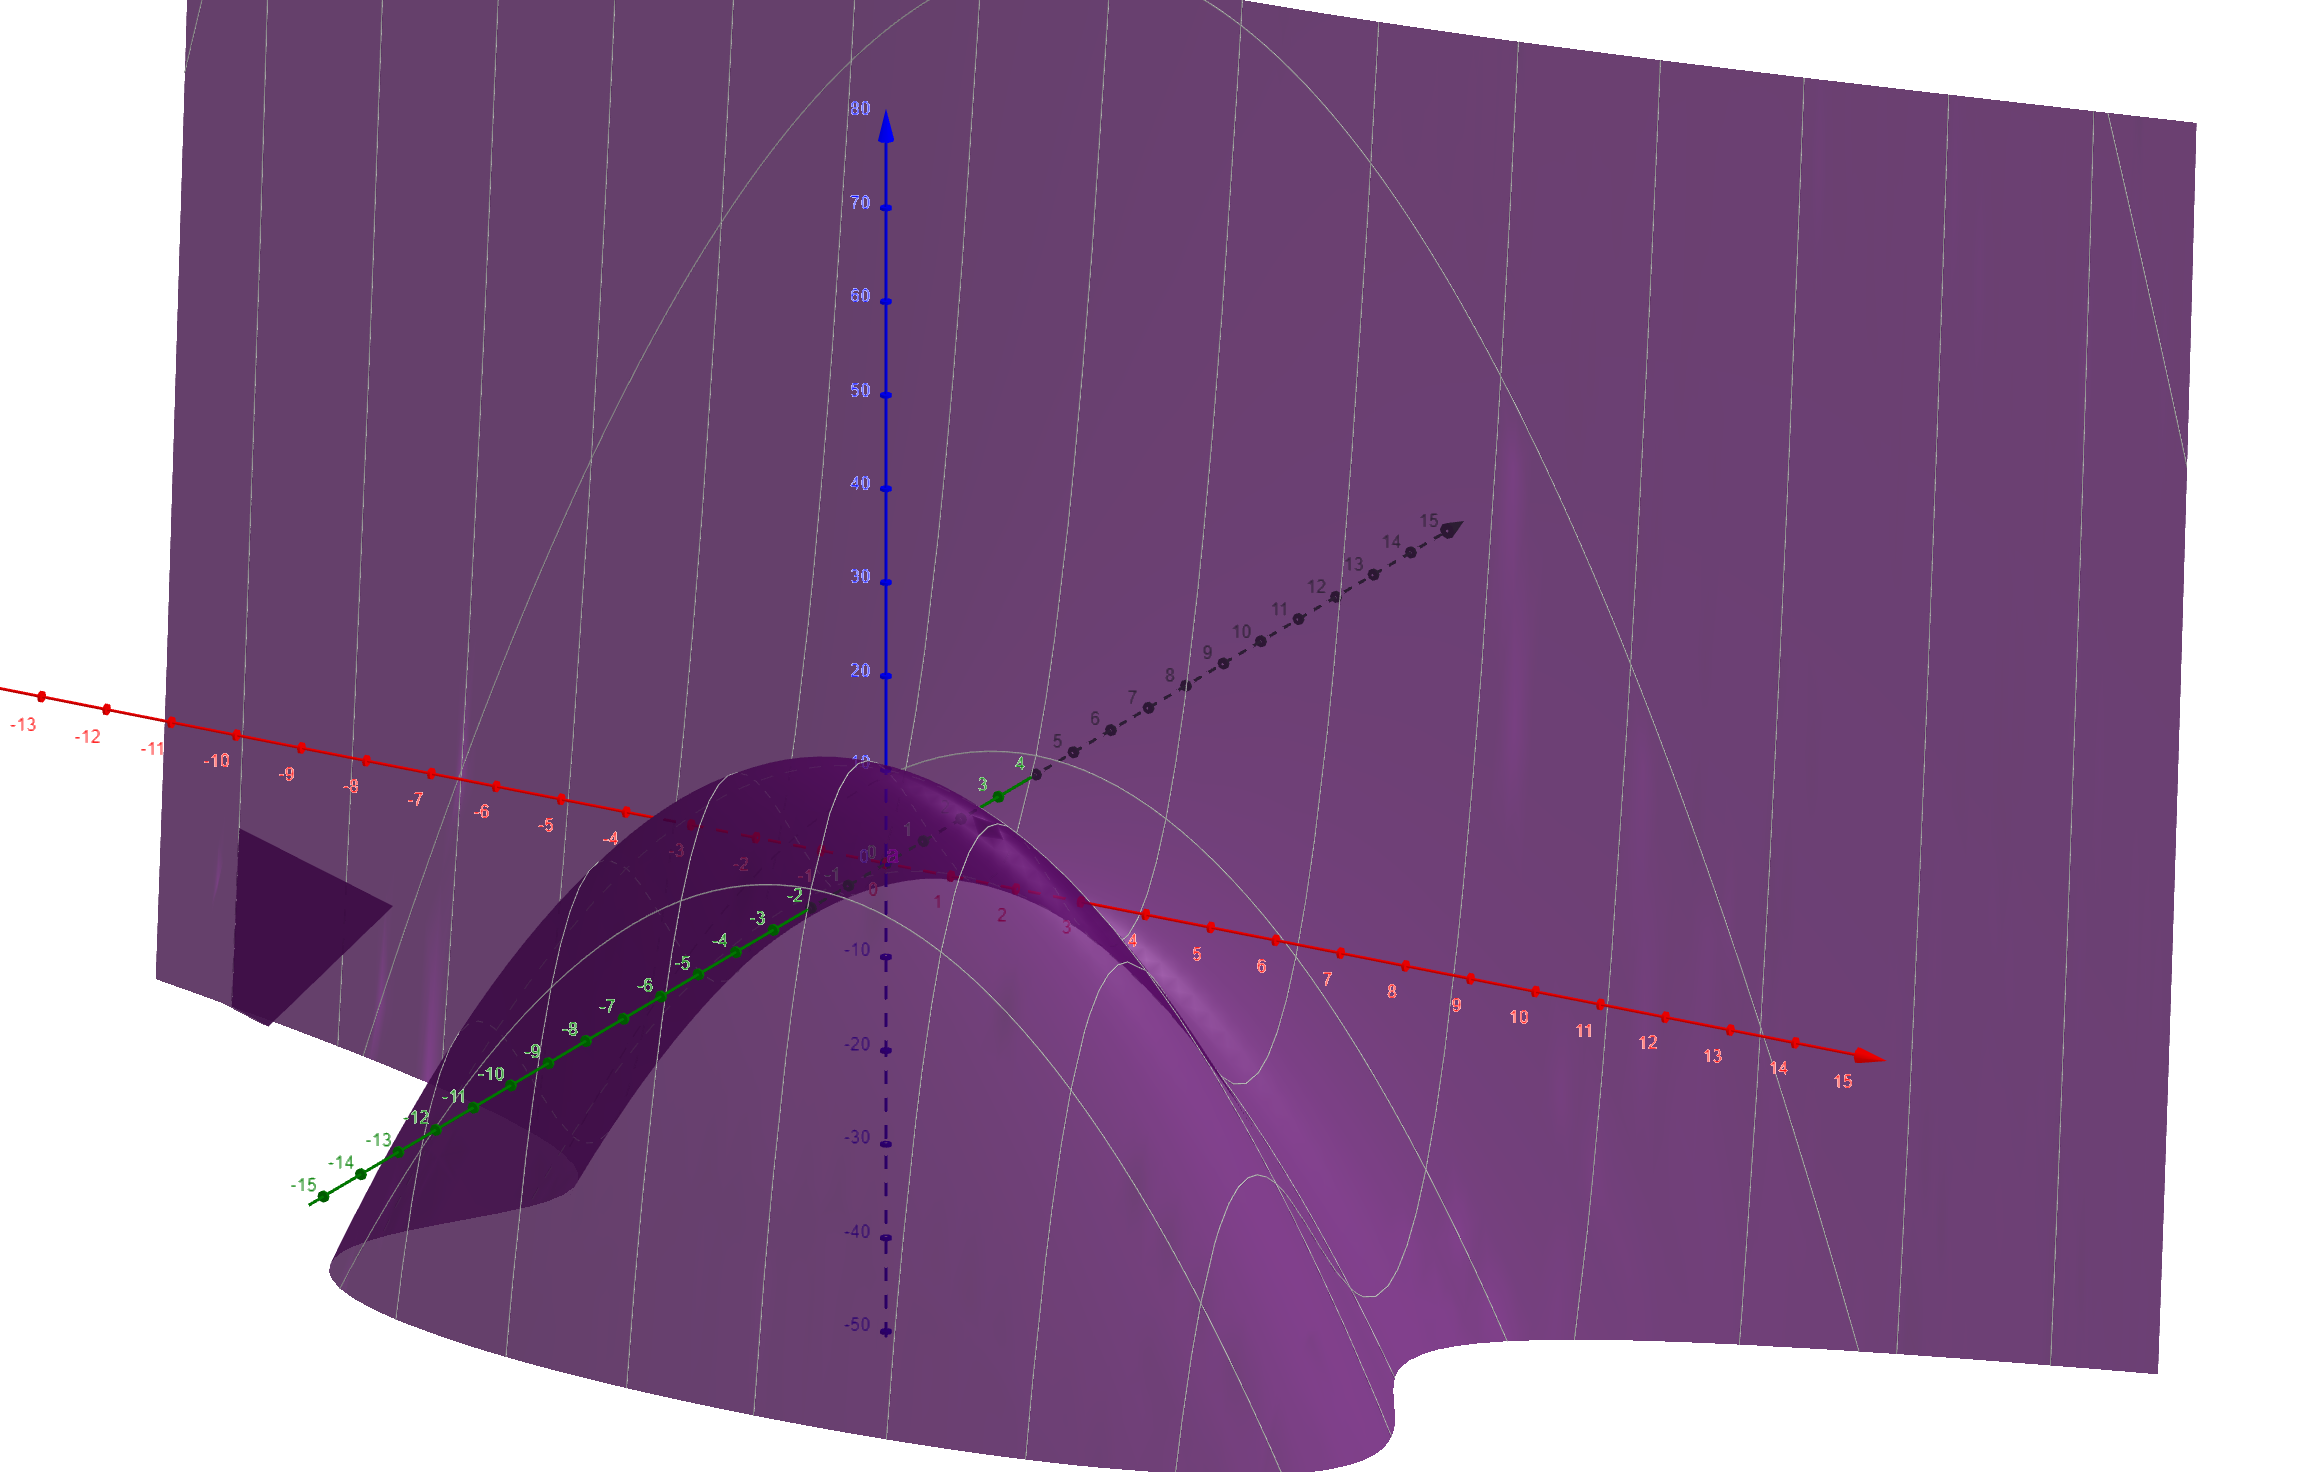
\includegraphics[scale=0.2]{Figures/surfaceex1} \\
 \href{https://www.geogebra.org/3d/gzy3xxgh}{Geogebra Link to Graph}
\end{center}
\end{example}

Visualizing 3-dimensional surfaces in 2-dimensional space can be a little tricky. We can, of course, use clever perspective, and Geogebra 3d lets us rotate the object and get a very good sense of it. Another useful technique is the \textbf{contour plot}. A common application of contour plots is topographic maps, where a contour plot is used to display elevation changes.

\begin{center}
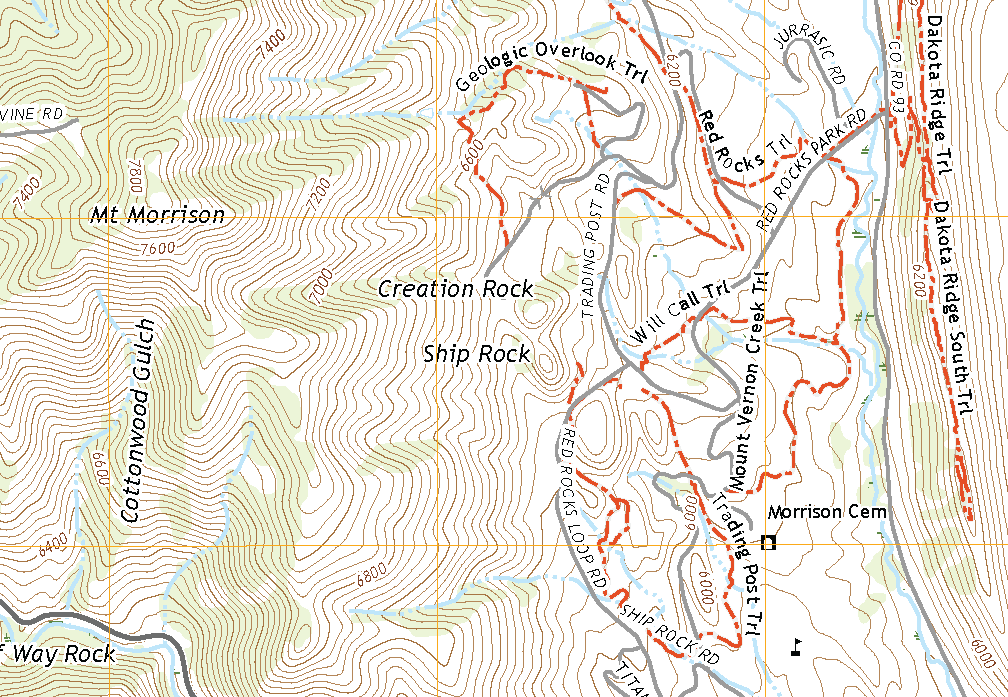
\includegraphics[scale=0.48]{Figures/redrocks}\\
Topographic Map of the area around Red Rocks in Morrison, Colorado.
\end{center}

A contour plot of a surface consists of a set of \textbf{level curves}, each of which are the intersection of the surface $f(x,y)=z$ and the plane $z=c$ for some $c\in\bbr$. That is, they are the collection of $2$-dimensional graphs, $f(x,y)=c$.

\begin{example}{Level Curves and Contour Plots}
Consider the same function as before, $f(x,y)=10-x^2+y^3-3y^2-6y$. We construct the following level curves:
\begin{align*}
-6=&10-x^2+y^3-3y^2-6y\\
-3=&10-x^2+y^3-3y^2-6y\\
0=&10-x^2+y^3-3y^2-6y\\
3=&10-x^2+y^3-3y^2-6y\\
6=&10-x^2+y^3-3y^2-6y\\
9=&10-x^2+y^3-3y^2-6y\\
12=&10-x^2+y^3-3y^2-6y.
\end{align*}
This yields the following contour plot:
\vspace{1em}
\begin{center}
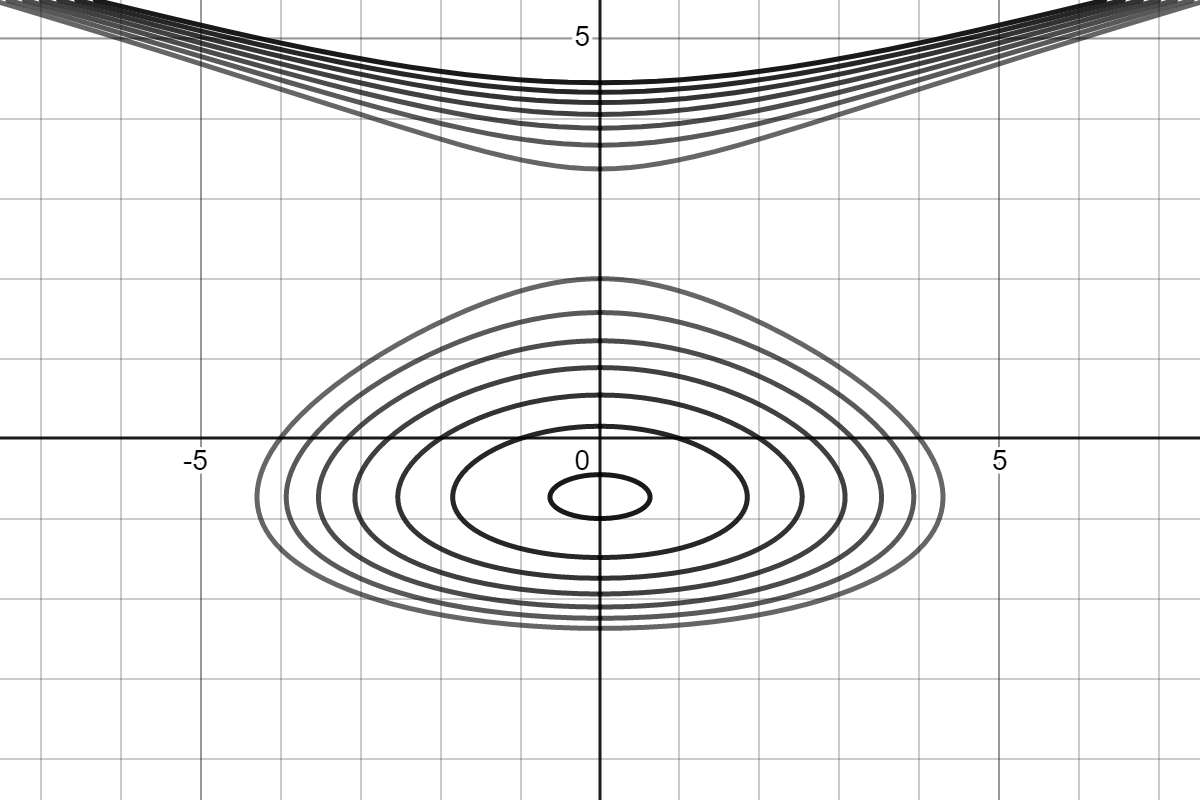
\includegraphics[scale=0.3]{Figures/contourex1}\\
Contour plot of $f(x,y)=10-x^2+y^3-3y^2-6y$.
\end{center}
\end{example}

\begin{exercise}{Level Curves}
\begin{enumerate}
\item Consider the function $f(x,y)=\sqrt{16-x^2-y^2}$. (don't graph this on geogebra yet!) Construct a set of level curves where $z=0$, $z=1$, $z=2$, $z=3$ and $z=4$, then produce a contour plot. Hint: You should be able to graph these without a computer graphing tool. Try squaring both sides of the level curve equation then rewriting it in the form $x^2+y^2=r^2$, which is a circle with radius $r$. 
\vspace{1em}
\item Can you conjecture what the graph of the surface looks like? Check your conjecture using Geogebra 3d.
\end{enumerate}
\end{exercise}

\subsection{Partial Derivatives and Tangent Planes}
Of course, this being a Calculus class, we probably want to get to some Calculus. So we start, as usual, with derivatives. However, we immediately run into a problem. When taking derivative of some function $y=f(x)$, we are interested in the derivative with respect to $x$: $f'(x)=\frac{dy}{dx}$. But what is $f'(x,y)$? Is it $\frac{d}{dx}f(x,y)$? What even does $\frac{d}{dx}f(x,y)$ even mean? Certainly, $y$ isn't a constant, but also it doesn't make any sense to use implicit differentiation, since $y$ isn't necessarily related to $x$ in some specific way. It turns out that in order to make sense of the situation, we must define a new type of derivative. Don't panic though, it's easier than it sounds! Basically, the \textbf{partial derivative} is a special type of derivative for surfaces that allows us to hold all other variables constant.

\begin{definition}{Partial Derivatives}
\begin{itemize}
\item The \textbf{partial derivative} of $f(x,y)$ with respect to $x$ is defined as the derivative of $f(x,y)$ with respect to $x$, while holding $y$ constant. It is written as $f_x$ or $\frac{\del f}{\del x}$. The partial differential operator with respect to $x$ is $\delx{}$. 
\vspace{1em}
\item The \textbf{partial derivative} of $f(x,y)$ with respect to $y$ is defined as the derivative of $f(x,y)$ with respect to $y$, while holding $x$ constant. It is written as $f_y$ or $\frac{\del f}{\del y}$. The partial differential operator with respect to $y$ is $\dely{}$. 
\end{itemize}
\end{definition}

\begin{exercise}{Partial Derivatives}
Consider $f(x,y)=\sqrt{16-x^2-y^2}$.
\vspace{1em}
\begin{enumerate}
\item Find $f_x$, the partial of $f$ with respect to $x$.
\vspace{1em}
\item Find $f_y$, the partial of $f$ with respect to $y$.
\end{enumerate}
\end{exercise}

The partial derivative acts somewhat like the regular derivative from Calculus I, but deals with an issue inherent to the situation-- the ``slope" or rate of change on a surface depends entirely on which direction you are going along. The partial with respect to $x$ tells us the ``slope" (or rate of change of $z$ with respect to $x$) as we move parallel to the $x$-axis, while the partial with respect to $y$ tells us the ``slope" (or rate of change of $z$ with respect to $y$) as we move parallel to the $y$-axis. These two ``slopes" come together to generate the equation of the \textbf{tangent plane}.

Note that when talking about planes in this section, we will not be using standard form, exactly. Instead, we will be presenting planes as some $z=f(x,y)$. So then, the plane $ax+by+cz=d$ would be written as $$f(x,y)=\frac{d}{c}-\frac{a}{c}x-\frac{b}{c}y.$$

\begin{definition}{Tangent Plane}
Let $f(x,y)$ be a surface. Then the plane tangent to $f(x,y)$ at the point $\big(x_0,y_0,f(x_0,y_0)\big)$ is $$\ell(x,y)=f(x_0,y_0)+f_x(x_0,y_0)(x-x_0)+f_y(x_0,y_0)(y-y_0). $$
\end{definition}

\begin{exercise}{Tangent Plane Equation}
Consider a function $f(x,y)$ and a point on that surface, $\big(x_0,y_0,f(x_0,y_0)\big)$. Then the partial with respect to $x$ at $(x_0,y_0)$ is $f_x(x_0,y_0)$ and the partial with respect to $y$ at $(x_0,y_0)$ is $f_y(x_0,y_0)$.
\vspace{1em}
\begin{enumerate}
\item Explain why the vectors $$\vcf_x=\bmat{1\\0\\f_x(x_0,y_0)}\text{ and } \vcf_y=\bmat{0\\1\\f_y(x_0,y_0)}$$
are parallel to the tangent plane to $f(x,y)$ at $(x_0,y_0)$.
\vspace{1em}
\item Using those two vectors and the point $\big(x_0,y_0,f(x_0,y_0)\big)$, give the equation of the tangent plane in vector dot product form, $$a(x-x_0)+b(y-y_0)+c(z-z_0)=0. $$
\item Solve the above equation of the plane for $z$ and show that you get the equation of the tangent line from the definition above.
\end{enumerate}
\end{exercise}

\begin{exercise}{Tangent Planes}
Find the equation of the plane tangent to $f(x,y)=\sqrt{16-x^2-y^2}$ at the point $(1,1)$.
\end{exercise}

We can, of course, take multiple partial derivatives in the same way that we can take multiple regular derivatives. However, this brings up a new possibility of \textit{mixed} partial derivatives.

\begin{definition}{Multiple Partial Derivatives}
Let $z=f(x,y)$ be an infinitely differentiable surface.
\vspace{1em}
\begin{itemize}
\item The second partial derivative with respect to $x$ is defined as $$f_{xx}(x,y)=\delx{}\big(f_x(x,y)\big). $$
\item The second partial derivative with respect to $y$ is defined as $$f_{yy}(x,y)=\dely{}\big(f_y(x,y)\big). $$
\item The mixed partial derivatives are defined as
$$f_{xy}(x,y)=\dely{}\big(f_x(x,y)\big),\text{ and }f_{yx}(x,y)=\delx{}\big(f_y(x,y)\big),$$ depending on whether we take the $x$ partial or the $y$ partial first.
\end{itemize}
\end{definition}

In general, the partial differential operators of different variables do not commute. However, in practice the two mixed partials are \textit{often} equal. The conditions for this are given by the following theorem of Clairaut and Schwarz,
 (Clairaut being one of the first to prove it and Schwarz being the first rigorous proof).
 
 \begin{theorem}{\hypertarget{cs}{Clairaut-Schwarz Theorem}}
Let $f(x,y)$ be a function $f:D\to\bbr$ where $D$ (the domain) is a subset of $\bbr^2$. Let $(x_0,y_0)$ be in $D$. Then, if some neighborhood of $(x_0,y_0)$ is contained in $D$ and $f_{xy}$ and $f_{yx}$ are continuous on that neighborhood, $$f_{xy}(x_0,y_0)=f_{yx}(x_0,y_0). $$
 \end{theorem}

 Note: A neighborhood is a way of saying some collection of all the points near another point. You can think of it like an open disk (i.e. all the points that are within $\varepsilon$ of $(x_0,y_0)$,) but a neighborhood need not be a regular shape. We could just state a stronger version of this theorem with an open rectangle or open disk, but I think neighborhood is a very useful and intuitive topographical term!
 
 Regardless, since most of the functions we see are continuous almost everywhere and infinitely differentiable almost everywhere, the \textbf{mixed partials are almost always equal.}
 
 \begin{exercise}{An Example of Clairaut-Schwarz Working!}
 Consider the function $$f(x,y)=\sin(x^2y^3).$$
 \begin{enumerate}
 \item Find $f_{xy}(x,y)$.
 \vspace{1em}
 \item Find $f_{yx}(x,y)$.
 \vspace{1em}
 \item Verify the criteria for Clairaut-Schwarz. That is, is $f(x,y)$ continuous? Are the mixed partials continuous?
 \vspace{1em}
 \item Verify the result for Clairaut-Schwarz. Are the two mixed partials equal?
 \end{enumerate}
 \end{exercise}


\subsection{Critical Points and the Second Derivative Test}
To begin the process of optimization, we must first begin the same way we did in Calculus I. We wish to identify places where a surface has a maximum or minimum, i.e. the apex of a peak or bottom of a valley. To do so, we must identify critical points. In Calculus I, the critical points were the places where the derivative could change signs, that is, the derivative was zero or did not exist. We expand this idea. But first, lets introduce a useful characterization of the partial derivatives of a surface $f$: the \textbf{gradient}.

\begin{definition}{Gradient}
Let $f(\vcx)$ be a function $f:D\to \bbr$ where $D$ is a subset of $\bbr^n$. That is, $f$ is a function with an $n$-dimensional vector input. Then the \textbf{gradient} of $f(\vcx)$, written $\nabla f(\vcx)$ is defined as the $n$-dimensional vector:
$$\nabla f(\vcx)=\bmat{\frac{\del f}{\del x_1}\\ \frac{\del f}{\del x_2}\\ \vdots \\ \frac{\del f}{\del x_n}}. $$
In particular, if $f(x,y)$ is a surface in 3-d space, $$\nabla f(x,y)=\bmat{f_x\\f_y}.$$
\end{definition}

We then use the gradient to define our critical points.

\begin{definition}{Critical Points}
Let $f(x,y)$ be a differentiable surface. Then if $\nabla f(x_0,y_0)$ does not exist, or $\nabla f(x_0,y_0)=\vzero$, we say that $f(x,y)$ has a critical point at $(x_0,y_0)$.
\end{definition}

Much like in Calculus I, a critical point is necessary for a local maximum or minimum, but not sufficient. While we certainly have the same issues that arise from zeros where the derivative does not change sign, we also get a new issue, saddle points. 

\begin{example}{Critical Points}
Recall the function $f(x,y)=10-x^2+y^3-3y^2-6y$.
\vspace{1em}
\begin{center}
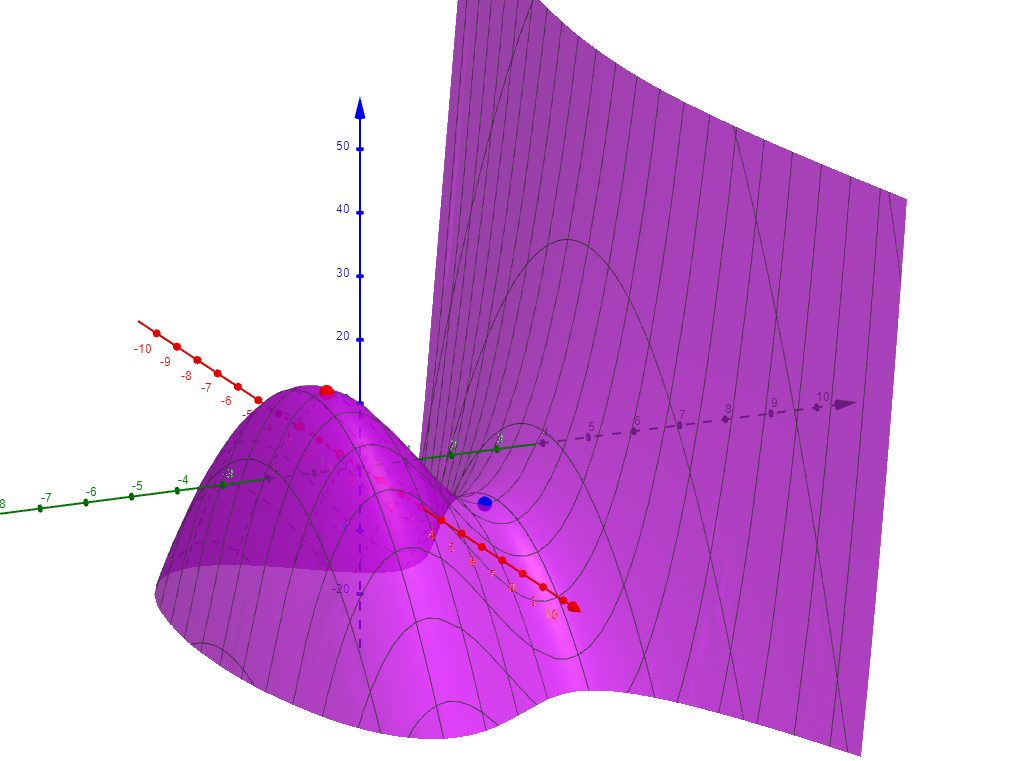
\includegraphics[scale=0.5]{Figures/surfaceex2} \\
 \href{https://www.geogebra.org/3d/ekkscrcb}{Geogebra Link to Graph}
\end{center}
Let's take our gradient:
$$\nabla f(x,y)=\bmat{-2x\\3y^2-6y-6} $$
Note that $\nabla f=0$ if $x=0$ and $y=1\pm\sqrt{3}$. This gives us two critical points, one at $(0,1+\sqrt{3})$ and the other at $(0,1-\sqrt{3})$. But looking at the graph, it is clear that $f$ has a local maximum at $(0,1-\sqrt{3})$ (the red dot), but at $(0,1+\sqrt{3})$ there is a \textbf{saddle point} (the blue dot).
\end{example}

\begin{exercise}{The Same Semi-sphere}
Consider, again, the function $$f(x,y)=\sqrt{16-x^2-y^2}.$$
Find the critical points of $f(x,y)$. You should find one point where $\nabla f=\vzero$, and an infinite family of points where $\nabla f$ doesn't exist.
\end{exercise}

You may recall that in Calculus I we had multiple ways of analytically categorizing critical points. In particular, we had a First Derivative Test (where we checked to see if the first derivative changed signs at our critical point), and a Second Derivative Test, where we checked the value of the second derivative. Unfortunately, there is no multivariate equivalent to the first derivative test. In particular, we would have to check every single possible path along the surface through our critical point to make sure that the derivative changed signs, which isn't really feasible. However, the second derivative test yields a multivariate version.

\begin{definition}{Second Derivative Test, Multivariable Edition}
Let $f(x,y)$ be a surface which has continuous second partials. Then define the discriminant, $$D(x,y)=f_{xx}f_{yy}-f_{xy}f_{yx}.$$ Note: Our condition here is the same as the Clairaut-Schwarz condition, so $f_{xy}=f_{yx}$, and so our discriminant is often written: $$D(x,y)=f_{xx}f_{yy}-(f_{xy})^2.$$ Let $f$ have a critical point at $(x_0,y_0)$. Then:
\vspace{1em}
\begin{itemize}
\item If $D(x_0,y_0)<0$, $f$ has a saddle at $(x_0,y_0)$.
\vspace{1em}
\item If $D(x_0,y_0)=0$, the test gives no information.
\vspace{1em}
\item If $D(x_0,y_0)>0$ and $f_{xx}(x_0,y_0)>0$ (or $f_{yy}(x_0,y_0)>0$), $f$ has a local minimum at $(x_0,y_0)$.
\vspace{1em}
\item If $D(x_0,y_0)>0$ and $f_{xx}(x_0,y_0)<0$ (or $f_{yy}(x_0,y_0)<0$), $f$ has a local maximum at $(x_0,y_0)$.
\end{itemize}
\end{definition}

\begin{exercise}{Clarifying the Second Derivative Test}
If $D(x_0,y_0)>0$, then the second derivative test can either check $f_{xx}$ or $f_{yy}$ to categorize the extrema. These are interchangeable because if $f_{xx}(x_0,y_0)>0$, then $f_{yy}(x_0,y_0)>0$ also. Why? (hint: the discriminant being positive here matters!)
\end{exercise}

\begin{example}{The Same Old}
Again, recall $f(x,y)=10-x^2+y^3-3y^2-6y$. As before, this function has critical points at $(0,1-\sqrt{3})$ and $(0,1+\sqrt{3}$. Lets compute our second partials and apply the second derivative test.
\begin{align*}
f_{xx}(x,y)=&-2\\
f_{yy}(x,y)=&6y-6\\
f_{yx}(x,y)=f_{xy}(x,y)=&0.
\end{align*}
Then \begin{align*}
D(x,y)=&(-2)(6y-6)-(0)(0)\\
=&-12y+12
\end{align*}
Note that it's often easier to evaluate the individual second derivatives rather than finding an explicit expression for $D(x,y)$. Let's go ahead and plug in our two critical points:
\begin{align*}
D(0,1-\sqrt{3})=&-12(1-\sqrt{3})+12\\
=&-12+12\sqrt{3}+12\\
=&12\sqrt{3}.\\
D(0,1+\sqrt{3})=&-12(1+\sqrt{3})+12\\
=&-12-12\sqrt{3}+12\\
=&-12\sqrt{3}.
\end{align*}
Since $D(0,1+\sqrt{3})<0$, $f$ has a saddle point at $(0, 1+\sqrt{3})$. On the other hand, since $D(0,1-\sqrt{3})>0$ and $f_{xx}(0,1-\sqrt{3})=-2<0$, $f$ has a local maximum at $(0, 1-\sqrt{3})$, which confirms our observations from the graphs above.
\end{example}

\begin{exercise}{The Semi-sphere... Again}
Consider, yet again, the surface $$f(x,y)=\sqrt{16-x^2-y^2}.$$ You found critical points earlier. The points where the partials don't exist defy the second derivative test, but you can use the second derivative test on the other critical point to categorize it.
\end{exercise}

\begin{exercise}{Finding Extrema}
Consider the surface $f(x,y)=x^2+xy+y^2-x+y+1$. Find all of the critical points of $f(x,y)$ and categorize them as saddles, minimums or maximums.
\end{exercise}

\begin{exercise}{I'm Sorry in Advance}
Consider the surface $$f(x,y)=x^3y^3-x^3y-xy^3+xy.$$
\begin{enumerate}
\item Take your partials and find all of the critical points of $f$. There should be \textit{thirteen}. (I told you I'm sorry! You may want to do some factoring by grouping.)
\vspace{1em}
\item Categorize each of the critical points as a saddle, minimum or maximum.
\vspace{1em}
\item Use the \href{https://www.geogebra.org/3d/nrqbqwen}{graph of the surface} to confirm your results from part 2.
\end{enumerate}
\end{exercise}


\subsection{Lagrange Multipliers and Optimization}
In Calculus I, you saw methods for constrained optimization. In particular, given a function with $n$ inputs and $n-1$ constraints, you could generally use the constraints to rewrite the function as a single input function, then simply find a maximum value. Using multivariate techniques, we can generalize these ideas a little further.

\begin{claim}{Gradient is Perpendicular to Level Curves}
Let $f(x,y)$ be a function, and $\nabla f(x,y)$ be the gradient of that function. Then for any $(x_0,y_0)$ in the domain of $f$, $\nabla f(x_0,y_0)$ is normal to (read perpendicular to) the level curve $f(x_0,y_0)=f(x,y)$ at $(x_0, y_0)$.
\end{claim}

That's an interesting claim. To justify it, we can both look at an example, and think about what the gradient represents. Firstly, let's think about the gradient. The gradient of $f$ is a vector function with a vector input. It takes some $(x,y)$ as input and returns a 2-dimensional vector as output. So a great way to visualize the gradient is as a slope field. This basically takes each $(x,y)$ input and draws a vector with the direction of $\nabla f$ at each point.

\vspace{1em}
\begin{center}
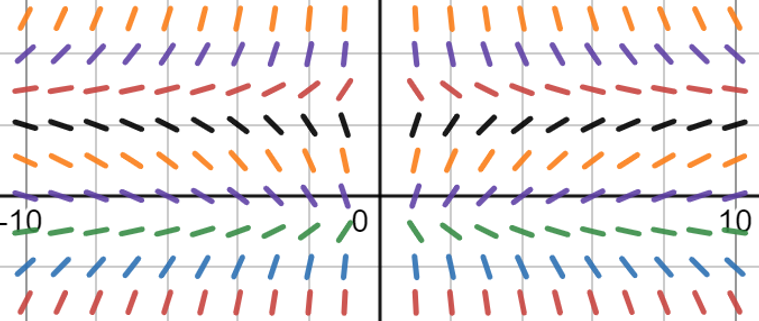
\includegraphics[scale=0.5]{Figures/slopefieldex1}
\\ Slope Field for $\nabla f$, where $f=10-x^2+y^3-3y^2-6y$.
\end{center}
\vspace{1em}

So what information does this actually tell us? Well, the gradient points us in the direction of maximal ascent of a surface. So if you're standing at $(x_0,y_0)$ on the surface of $f$, then the gradient tells you what direction you should turn to ascend as quickly as possible.

Another way to think of that is, if you're standing at $(x_0,y_0)$ on the surface of $f$, then consider the plane tangent to $f$ at $(x_0,y_0)$. This plane should have some ``flat" line you can walk along, some line parallel to the $xy$-plane. The gradient will be perpendicular to that line.

Let's look at an example!

\begin{example}{Gradient and Level Curves}
Let's keep using the function $f(x,y)=10-x^2+y^3-3y^2-6y$. We will consider the point at $x=1$, $y=1$. Then $f(x,y)=10-1^2+1^3-3(1)^2-6(1)=1$. Additionally, $$\nabla f(1,1)=\bmat{-2(1)\\3(1^2)-6(1)-6}=\bmat{-2\\-9}.$$
We can see the situation in the graph below. The black curve is the level curve $1=f(x,y)$. The blue vector is the gradient padded out with a $z$-coordinate of $0$, moved over to begin at $(1,1,1)$ for clarity. The red line is the line tangent to the normal curve. The purple plane is the tangent plane (not shown in the image below for clarity).
\vspace{1em}
\begin{center}
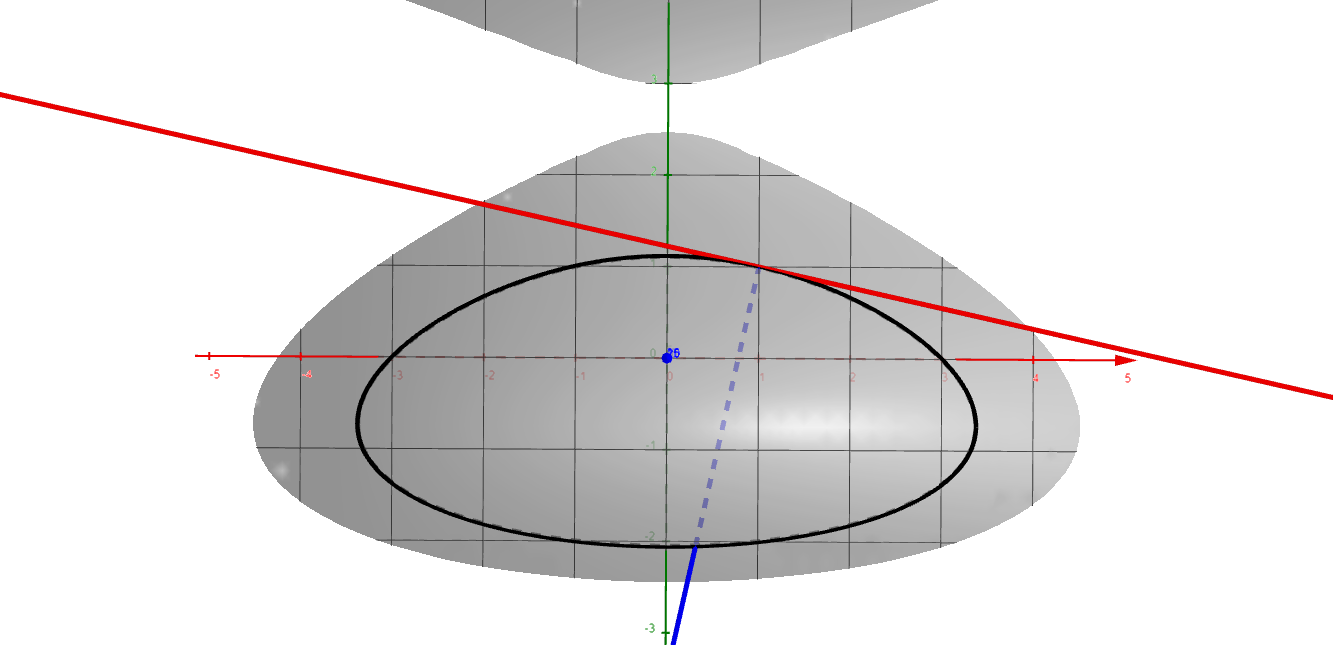
\includegraphics[scale=0.25]{Figures/normaltolevelex}\\
\href{https://www.geogebra.org/3d/w3hdn8w7}{Click Here for an interactable Geogebra Link.}
\end{center}
\vspace{1em}

If you go to the geogebra link, you can vary the values of $h$ and $k$ to explore this situation at an any given arbitrary $x=h$ and $y=k$. You should find that the gradient vector is always normal to the given level curve.

\vspace{1em}

But why is this the case? Let's try to get some intuition. Imagine you're standing at the point $A=(h,k,f(h,k))$ on this surface, and you want to climb to a higher altitude. The level curve at $A$ denotes the altitude that you are at, while the second level curve denotes the part of the surface that is at the higher altitude that you want to climb to.
\vspace{1em}
\begin{center}
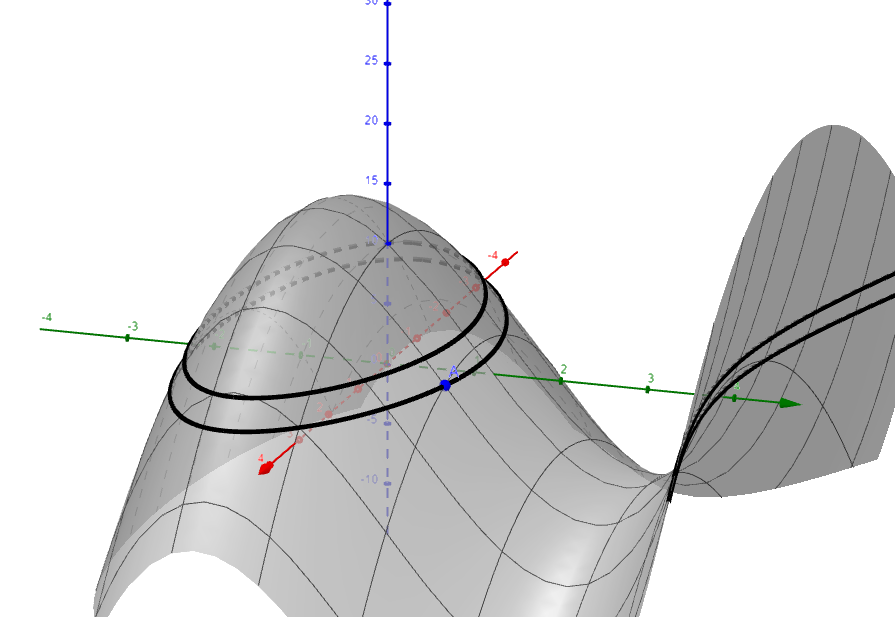
\includegraphics[scale=0.4]{Figures/gradperp1}\\
Point A and Level Curves.
\end{center}
\vspace{1em}
What direction should you head in to ascend as quickly as possible? Well, the direction to the closest point along the next level curve is perpendicular from your current level curve. 

\vspace{1em}

Let's consider the plane tangent to $f(x,y)$ at $A$. We learned in section 4.2 that the tangent plane should be parallel to the vectors $$\vcf_x=\bmat{1\\0\\f_x(h,k)}\text{ and } \vcf_y=\bmat{0\\1\\f_y(h,k)}.$$ We can calculate the cross product of those two vectors $$\vcf_y\times\vcf_x=\bmat{f_x(h,k)\\f_y(h,k)\\-1},$$ which is exactly the vector that is normal to the tangent plane. Since the line that is tangent to our level curve at $A$ is contained inside plane tangent to $f$ at $A$, this normal vector must be perpendicular to that line tangent to the level curve (the red line from the figure earlier in this example). Then notice that if you truncate off the $z$-coordinate from our normal vector, $$ \bmat{f_x(h,k)\\f_y(h,k)\\-1}\to \bmat{f_x(h,k)\\f_y(h,k)}=\nabla f(h,k).$$ This is exactly the gradient of $f$ evaluated at $(h,k)$. Therefore, the gradient gives us the direction that is perpendicular to our level curve, which points us in the direction of steepest ascent.
\vspace{1em}
\end{example}

Why does this matter? Well, it's key to a method of optimization called \textbf{Lagrange multipliers}. Essentially, given some surface $f(x,y)$ and a constraint curve $g(x,y)=c$, any maximum or minimum of the intersection of the surface and constraint will be found at a point where the gradient of the surface and the gradient of the constraint point in the same direction. We don't care about the magnitude of the gradients, so that introduces the nominal multiplier. More specifically:

\begin{theorem}{Lagrange Multipliers}
Let $z=f(x_1,\ldots, x_n)$ be a function and $c=g(x_1,\ldots,x_n)$ be a constraint curve. Then any max or min of $f$ along $g(x,y)=c$ will be found at a point satisfying the equation $$\nabla f=\lambda \nabla g $$ where $\lambda$ is some constant.
\end{theorem}

In particular, note that $\nabla f=\lambda \nabla g$ yields exactly $n$ equations with $n+1$ unknowns. So if you include the constraint itself, you have a system of equations with $n+1$ equations and $n+1$ unknowns, so it is theoretically possible to solve for all of your unknown values. In practice, these systems are often non-linear in multiple variables and extremely difficult to solve by hand, but can be solved by computers.

\begin{example}{A Calculus I Problem made Harder.}
Suppose we want to build a square bottomed box with a double thickness base and we have exactly $8$ square meters of materials. How should we build the box to maximize the volume contained in the box? First, let's start by identifying an objective function and a constraint curve. Here, our objective is volume. Since the base of the box is square, we can write our volume function as $$f(x,y)=x^2y.$$
Then our constraints should be the surface area of the box. We need a double thickness base, so we will have four sides of area $xy$, the top will be area $x^2$ and the bottom will need two slabs of area $x^2$. Since we have exactly 8 square meters of material, this leaves the constraint $$8=4xy+3x^2. $$ If you follow this \href{https://www.geogebra.org/3d/azxkj796}{Geogebra Link}, you'll be able to see a graph of the surface $f(x,y)$ and the constraint, $8=4xy+3x^2$. The intersection of these two surfaces is the path that we are trying to find the highest point along. To do that, we'll use our Lagrange multiplier to try to identify where our gradients are parallel. Note that in this case, $g(x,y)=4xy+3x^2$. So then our gradients in question are $$\nabla f(x,y)=\bmat{2xy\\x^2}, \text{ and }\nabla g(x,y)=\bmat{4y+6x\\4x} $$
and our Lagrange multiplier condition is $$\bmat{2xy\\x^2}=\lambda\bmat{4y+6x\\4x}. $$
This yields the following system of 3 unknowns and 3 equations:
\begin{align*}
2xy=&\lambda(4y+6x)\\
x^2=&4\lambda x\\
8=&4xy+3x^2.
\end{align*}
This system of equations yields that $x=\frac{2\sqrt{2}}{3}$ and $y=\sqrt{2}$. It also finds that $\lambda=\frac{\sqrt{2}}{6}$, which isn't necessary for our solution but a useful intermediary step. 
\end{example}

\begin{exercise}{Something Geometric}
Consider the surface $$f(x,y)=5+2x-y$$ and the constraint curve $$1=x^2+\frac{y^2}{4}.$$ Find the maximum and minimum points of the surface along the constraint curve. You can see this surface and constraint at this \href{https://www.geogebra.org/3d/dxtzfpca}{Geogebra link}.
\end{exercise}

\begin{exercise}{Revisiting Point to Plane}
While earlier in the semester we solved the question of point to plane using geometry and projections, we can also consider the idea of finding the distance between a point and a plane as a constrained optimization problem. In this case, the function we are seeking to minimize is the distance between an arbitrary point and the point in question, and the constraint is the equation of the plane itself. Let $P=(1,3,2)$ and consider the plane $-x+y-2z=3$. 
\vspace{1em}
\begin{itemize}
\item What is the function that gives the distance, $d$, between $P$ and an arbitrary point, $(x,y,z)$? 
\vspace{1em}
\item Note that if we just use the distance formula blindly, while we get a technically solvable problem, it's a very \textit{gross} solvable problem. However, there's a nice trick here. Explain why minimizing the \textit{square} of the distance is the same as minimizing the distance! 
\vspace{1em}
\item Now using $f(x,y,z)=d^2$ and the constraint $-x+y-2z=3$, use Lagrange multipliers to find the minimum distance between the point and plane. 
\vspace{1em}
\item Verify that your distance is correct by using the projection method we studied earlier in the semester!
\end{itemize}
\end{exercise}

\begin{exercise}{Something Economic}
The Cobb-Douglas production model seeks to define production as a function of labor and capital. Call $x$ the amount of labor and $y$ the amount of capital invested into a project. Then the total cost of the project is $$c=ax+by.$$ The Cobb Douglas (with slight simplification and some assumptions) model claims that $P(x,y)$, the amount of production as a factor of $x$ amount of labor and $y$ amount of capital will be of the form $$P(x,y)=x^\alpha y^{1-\alpha} $$ for some real $\alpha$. Use Lagrange multipliers to calculate how much labor and capital should be applied in order to maximize production. Your answer should be stated in terms of $a,b,c$ and $\alpha$.
\end{exercise}
\renewcommand\thesubsection{\thesection.\Alph{subsection}}
\setcounter{subsection}{18}
\subsection{Partial Derivatives Summary}

\begin{definition}{Partial Derivatives}
\begin{itemize}
\item The \textbf{partial derivative} of $f(x,y)$ with respect to $x$ is defined as the derivative of $f(x,y)$ with respect to $x$, while holding $y$ constant. It is written as $f_x$ or $\frac{\del f}{\del x}$. The partial differential operator with respect to $x$ is $\delx{}$. 
\vspace{1em}
\item The \textbf{partial derivative} of $f(x,y)$ with respect to $y$ is defined as the derivative of $f(x,y)$ with respect to $y$, while holding $x$ constant. It is written as $f_y$ or $\frac{\del f}{\del y}$. The partial differential operator with respect to $y$ is $\dely{}$. 
\end{itemize}
\end{definition}

\begin{definition}{Tangent Plane}
Let $f(x,y)$ be a surface. Then the plane tangent to $f(x,y)$ at the point $\big(x_0,y_0,f(x_0,y_0)\big)$ is $$\ell(x,y)=f(x_0,y_0)+f_x(x_0,y_0)(x-x_0)+f_y(x_0,y_0)(y-y_0). $$
\end{definition}

 \begin{theorem}{{Clairaut-Schwarz Theorem}}
Let $f(x,y)$ be a function $f:D\to\bbr$ where $D$ (the domain) is a subset of $\bbr^2$. Let $(x_0,y_0)$ be in $D$. Then, if some neighborhood of $(x_0,y_0)$ is contained in $D$ and $f_{xy}$ and $f_{yx}$ are continuous on that neighborhood, $$f_{xy}(x_0,y_0)=f_{yx}(x_0,y_0). $$
 \end{theorem}

 \begin{definition}{Gradient}
Let $f(\vcx)$ be a function with an $n$-dimensional vector input. Then the \textbf{gradient} of $f(\vcx)$, written $\nabla f(\vcx)$ is defined as the $n$-dimensional vector:
$$\nabla f(\vcx)=\bmat{\frac{\del f}{\del x_1}\\ \frac{\del f}{\del x_2}\\ \vdots \\ \frac{\del f}{\del x_n}}. $$
In particular, if $f(x,y)$ is a surface in 3-d space, $$\nabla f(x,y)=\bmat{f_x\\f_y}.$$
\end{definition}

 \begin{definition}{Critical Points}
Let $f(x,y)$ be a differentiable surface. Then if $\nabla f(x_0,y_0)$ does not exist, or $\nabla f(x_0,y_0)=\vzero$, we say that $f(x,y)$ has a critical point at $(x_0,y_0)$.
\end{definition}

\begin{definition}{Second Derivative Test, Multivariable Edition}
Let $f(x,y)$ be a surface which has continuous second partials. Then define the discriminant, $$D(x,y)=f_{xx}f_{yy}-f_{xy}f_{yx}.$$ Let $f$ have a critical point at $(x_0,y_0)$. Then:
\vspace{1em}
\begin{itemize}
\item If $D(x_0,y_0)<0$, $f$ has a saddle at $(x_0,y_0)$.
\vspace{1em}
\item If $D(x_0,y_0)=0$, the test gives no information.
\vspace{1em}
\item If $D(x_0,y_0)>0$ and $f_{xx}(x_0,y_0)>0$ (or $f_{yy}(x_0,y_0)>0$), $f$ has a local minimum at $(x_0,y_0)$.
\vspace{1em}
\item If $D(x_0,y_0)>0$ and $f_{xx}(x_0,y_0)<0$ (or $f_{yy}(x_0,y_0)<0$), $f$ has a local maximum at $(x_0,y_0)$.
\end{itemize}
\end{definition}

\begin{theorem}{Lagrange Multipliers}
Let $z=f(x_1,\ldots, x_n)$ be a function and $c=g(x_1,\ldots,x_n)$ be a constraint curve. Then any max or min of $f$ along $g(x,y)=c$ will be found at a point satisfying the equation $$\nabla f=\lambda \nabla g $$ where $\lambda$ is some constant.
\end{theorem}

\subsubsection*{Companion Videos by Ken Monks}
\begin{itemize}
\item \href{https://www.youtube.com/watch?v=7M0O_Y88wYM}{Surfaces and Contour Plots.}
\item \href{https://www.youtube.com/watch?v=LmDz71ssyEA}{Partial Derivatives of Surfaces and Tangent Planes.}
\item \href{https://www.youtube.com/watch?v=rNK0GXjsjEg}{Critical Points of Surfaces.}
\item \href{https://www.youtube.com/watch?v=ontRtIlXu3A}{Gradients of Surfaces.}
\item \href{https://www.youtube.com/watch?v=26h_eWSdcrA}{Lagrange Multipliers.}
\item \href{https://www.youtube.com/watch?v=JVnyQUNnuSU}{Lagrange Multipliers and the Multivariable Extreme Value Theorem.}
\end{itemize}

\renewcommand\thesubsection{\thesection.\arabic{subsection}}
\renewcommand\thesubsection{\thesection.\Alph{subsection}}
\setcounter{subsection}{17}
\subsection{Partial Derivatives Homework and Miscellaneous Practice}

\begin{exercise}{Level Curves}
Consider the function $f(x,y)=16-x^2-4y^2$. Describe the level curves of $f(x,y)$ at $z=-9, z=0, z=7, z=12$ and $z=16$. Use this information to describe the shape of the surface.  
\end{exercise}

\begin{pexercise}{Partial Derivatives 1}%pon
Consider the function $f(x,y)=\cos(xe^{y^2})$ Find both first partial derivatives of $f$.
\end{pexercise}

\begin{pexercise}{Partial Derivatives 2}%pon
Consider the function $f(x,y)=\ln\left(\frac{y}{x}\right)+\ln\left(\frac{1}{x+y}\right)$ Find both first partial derivatives of $f$.
\end{pexercise}

\begin{exercise}{Tangent Plane}
Find the equation of the plane tangent to $f(x,y)=16-x^2-4y^2$ at $(1,-1)$.
\end{exercise}

\begin{exercise}{Multiple Partials}
Let $f(x,y)=\cos(xy+x)$.
\begin{enumerate}
\item Find $f_{xx}(x,y)$.
\item Find $f_{yy}(x,y)$.
\item Find $f_{xy}(x,y)$.
\end{enumerate}
\end{exercise}

\begin{exercise}{Critical Points 1}
Consider the function $f(x,y)=x^2-4x+y^3-3y^2-y$. Find the critical points of $f(x,y)$ and classify them using the second derivative test.
\end{exercise}

\begin{pexercise}{Critical Points 2}%pon
Consider the function $f(x,y)=2y-9x-xy+5x^2+y^2$. Find the critical points of $f(x,y)$ and classify them using the second derivative test.
\end{pexercise}

\begin{pexercise}{Lagrange 1}%pon
Find the maximum and minimum values of $f(x,y)=3x-6y$ subject to the constraint $4x^2+2y^2=25$.
\end{pexercise}

\begin{exercise}{Lagrange 2}
Suppose you are trying to maximize the volume of a box given 6 square meters of material. Note that the volume of the box is $f(x,y,z)=xyz$. Set up, but do not solve the Lagrange multiplier system of equations needed to maximize the volume.
\end{exercise}
\renewcommand\thesubsection{\thesection.\arabic{subsection}}

\section{Multiple Integrals}
\subsection{Multiple Integrals}
In an analogue to the area beneath a curve, the integral of a surface represents the volume beneath the surface on an open rectangle.

\begin{definition}{Double Integral}
Somewhat informally, we define the double integral over the rectangle $R$ of the function $f(x,y)$ as the area beneath the surface $f(x,y)$ bounded by the rectangle $R$ in the $xy$-plane, and it is written $$\iint_R f(x,y) \ dA $$  
\end{definition}

Technically, the double integral is defined using Riemann sums, in much the same way that the integral was defined in Calculus I. The primary difference is that the rectangles are now three dimensional rectangular prisms, and the sums must be taken over both an $x$ and a $y$ partition. For a more complete definition of the double integral, see the companion video \href{https://www.youtube.com/watch?v=ga7g3kuoGBY}{here.} However, Riemann sums are, as always, bulky. Due to the relative independence of the $x$ and $y$ variables, we can compute the double integral using the following theorem of Fubini.

\begin{theorem}{Fubini's Theorem}
Let $f(x,y)$ be continuous on the rectangle $R=[a,b]\times[c,d]$. Then $$\iint_R f(x,y)\ dA=\int_{a}^{b}\int_{c}^{d}f(x,y)\ dy\ dx=\int_{c}^{d}\int_{a}^{b}f(x,y)\ dx\ dy.$$ In other words, we can compute the double integral through iterated integration with respect to $x$ then with respect to $y$.
\end{theorem}

Note that much like partial derivatives, these ``partial" integrals assume you are holding all other variables constant.

\begin{example}{Double Integral on a Rectangle}
Consider the function $f(x,y)=xy$ on the rectangle $[2,4]\times [1,2]$. That is, the rectangle that has one corner at the point $(2,1)$ and the opposite corner at the point $(4,2)$. We can compute the area beneath this curve:
\begin{align*}
\iint_{R}xy\ dA=&\int_{1}^2\int_2^4 xy\ dx\ dy\\
=&\int_{1}^2\Bigg[\frac{x^2y}{2} \Bigg]_{x=2}^{x=4} \ dy\\
=&\int_1^2\frac{16y}{2}-\frac{4y}{2} \ dy\\
=&\int_1^2 6y\ dy\\
=&\Bigg[3y^2\Bigg]_{y=1}^{y=2}\\
=&12-3\\
=&9.
\end{align*}
\end{example}

\begin{pexercise}{Double Integrals}
Set up and evaluate the double integral $\iint_R f(x,y)\ dA$ for the following surfaces and rectangles.
\vspace{1em}
\begin{enumerate}
\item $f(x,y)=6xy^2$, $R=[2,4]\times [1,2]$.%pon
\vspace{1em}

\item $f(x,y)=\dfrac{1}{(2x+3y)^2}$, $R=[0,1]\times[1,2]$.%pon
\vspace{1em}

\item $f(x,y)=xe^{xy}$, $R=[-1,2]\times[0,1]$. Hint: The order of integration being commutative might save you a headache here! %pon
\end{enumerate}
\end{pexercise}

Rectangular regions are pretty straightforwards, but unfortunately not every region is rectangular. In particular, we can handle regions where the $x$ bounds can be written as some functions of $y$, i.e. $g(y)\leq x\leq h(y)$ or where the $y$ bounds can be written as some functions of $x$, i.e. $g(x)\leq y\leq h(x)$.

\begin{definition}{Non-Rectangular Double Integrals}
\begin{itemize}
\item Let $f(x,y)$ be continuous on the domain $D=\{(x,y):\ a<x<b,\ g(x)<y<h(x) \}.$ Then: $$\iint_D f(x,y)\ dA=\int_{a}^{b}\int_{g(x)}^{h(x)}f(x,y)\ dy \ dx. $$
\item Let $f(x,y)$ be continuous on the domain $D=\{(x,y):\ g(y)<x<h(y).\ a<y<b \}. $ Then: $$\iint_{D}f(x,y)\ dA=\int_{a}^b\int_{g(y)}^{h(y)}f(x,y)\ dx \ dy. $$
\end{itemize}
\end{definition}

\begin{example}{A Non-Rectangular Region}
Consider the right unit tetrahedron with it's right angle corner at the origin. That is, the volume bounded by the planes: \begin{align*}
x+y+z=&1\\
x=&1\\
y=&1\\
z=&1.
\end{align*}
You can look at this \href{https://www.geogebra.org/3d/bndxps3v}{here.} We can set this up as the surface $f(x,y)=1-x-y$ (this is just solving the plane $x+y+z=1$ for $z$.) on the region $D=\{(x,y):\ 0\leq x\leq 1,\ 0\leq y \leq 1-x \}.$ Then we can set up our double integral:
$$\iint_D 1-x-y\ dA=\int_{0}^1\int_0^{1-x} 1-x-y \ dy\ dx. $$
Then we can solve this integral:
\begin{align*}
\int_{0}^1\int_0^{1-x} 1-x-y \ dy\ dx=&\int_0^1\Bigg[y-xy-\frac{y^2}{2}\Bigg]_{y=0}^{y=1-x}\ dx\\
=&\int_{0}^1 (1-x)-x(1-x)-\frac{(1-x)^2}{2} \ dx\\
=&\int_0^1 1-2x+x^2-\frac{1-2x+x^2}{2} \ dx\\
=&\int_0^1 \frac{1-2x+x^2}{2}\ dx\\
=&\Bigg[\frac{x-x^2+\frac{x^3}{3}}{2}\Bigg]_{x=0}^{x=1}\\
=&\frac{1-1+1/3}{2}\\
=&\frac{1}{6}
\end{align*}
Since the shape is a triangular pyramid, the volume should be $\frac{1}{3}bh$. The base is area 1/2, the height is 1, so a volume of $1/6$ makes sense!
\end{example}

\begin{exercise}{More Irregular Domains}
Set up and evaluate the double integral $\iint_D f(x,y)\ dA$ for the following surfaces and rectangles.
\vspace{1em}
\begin{enumerate}
\item $f(x,y)=e^{\frac{x}{y}}$. $D=\{(x,y):\ y\leq x\leq y^2 ,\ 0\leq y\leq 2 \}$.
\vspace{1em}
\item $f(x,y)=xy-y^2$, $D$ is the region bounded by $y=\sqrt{x}$ and $y=x^2$.
\vspace{1em}
\item $f(x,y)=2xy$, $D$ is the triangle with vertices at $(0,0)$, $(1,2)$ and $(2,1)$. Hint: You may want to split this up into two separate integrals to make one of your bounds a pair of constants on each integral!
\end{enumerate}
\end{exercise}

We can expand the ideas of double integrals into triple integrals and beyond.

\begin{definition}{Triple Integral on a Rectangular Prism}
Let $f(x,y,z)$ be a function and $R$ be the rectangular prism $R=[a,b]\times[c,d]\times[e,f]$. Then we can evaluate the triple integral $$\iiint_R f(x,y,z)\ dV=\int_e^f\int_c^d\int_a^b f(x,y,z) \ dx \ dy \ dz.$$
You can also order the integration any of the 6 possible ways!
\end{definition}

\begin{exercise}{A Triple Integral}
Let $R=[0,3]\times[0,2]\times[0,1]$. Evaluate $$\iiint_R 4xyz \ dV.$$
\end{exercise}

\begin{definition}{Triple Integral on an Arbitrary Region}
Note: We examine here an integral where the $z$ bounds are a function of $x$ and $y$, and the $y$ bounds are a function of $x$. There are 6 possible parameterizations, and all resolve similarly, but for brevity, we'll stick to one case here!

\vspace{1em}

Let $f(x,y,z)$ be a function and $D$ be a region in $3$-space such that $$D=\big\{(x,y,z): \ a\leq x\leq b,\ g(x)\leq y\leq h(x),\ G(x,y)\leq z\leq H(x,y)  \big\}.$$ Then the triple integral can be evaluated as the iterated integral: $$\iiint_D f(x,y,z)\ dV=\int_a^b\int_{g(x)}^{h(x)}\int_{G(x,y)}^{H(x,y)}f(x,y,z)\ dz \ dy \ dx. $$
\end{definition}

\begin{pexercise}{A Triple Integral on a Non-Rectangular Region}%pon
Let $D=\{(x,y,z):\ 0\leq x\leq 2,\ 0\leq y \leq 1,\ 0\leq z\leq 4-xy \}$. Evaluate $$\iiint_D 3-4x\ dV.$$
\end{pexercise}

\begin{pexercise}{Another Triple Integral on a Non-Rectangular Region}%pon
Let $D=\{(x,y,z):\ 0\leq x\leq \frac{z}{2},\ 0\leq y\leq 10-2z,\ 0\leq z\leq 5 \}$. Evaluate $$\iiint_D 12y-8x\ dV. $$
\end{pexercise}

\subsection{Change of Variables and the Jacobian}
\begin{example}{Annoying Example}
Lets consider the volume beneath the surface $f(x,y)=1$ where $D$ is the disk of radius 1. Clearly this is just a cylinder with radius 1 and height 1, and our volume should simply be $\pi$. But for the sake of example, lets set this up as a double integral.
$$\iint_D 1 \ dA=\int_{-1}^{1}\int_{-\sqrt{1-x^2}}^{\sqrt{1-x^2}}1\ dy\ dx. $$
Evaluating the inner integral leads us quickly to:
$$\int_{-1}^{1}2\sqrt{1-x^2}\ dx $$ which you may recall from Calculus II as a tedious trig sub where $x=\sin\theta$. There has to be an easier way!
\end{example}

In fact, there is an easier way, related to a method of integration you've been using for almost as long as you've been integrating! Remember the method of $u$-substitution, where you evaluate a tricky single integral by substituting some $u$ for $x$. Of course, you have to be careful-- and there's a trade off. When doing your $u$ substitution, you must not only replace $x$ with $u$, but also replace $dx$ with $du$. We use an expansion of this technique to do substitutions, or changes of variables for multiple integrals.

Why are these changes of variables useful? Well, often times an annoying object in one set of variables is a much less annoying object in another set of variables.

\begin{example}{An Ellipse No More}
Consider the ellipse $x^2+\frac{y^2}{36}=1.$ If we use the change of variables $x=\frac{u}{2}$ and $y=3v$, then we substitute:
\begin{align*}
x^2+\frac{y^2}{36}=&1\\
\left(\frac{u}{2}\right)^2+\frac{(3v)^2}{36}=&1\\
\frac{u^2}{4}+\frac{v^2}{4}=&1\\
u^2+v^2=4.
\end{align*}
This is a circle with radius 2.
\end{example}

\begin{exercise}{A Transformation}
Consider the region that is the triangle with vertices at $(0,0)$, $(1,2)$ and $(2,1)$. This is the region bounded by the lines \begin{align*}
y=&2x\\
y=&\frac{1}{2}x\\
y=&3-x.
\end{align*}
Use the transformation $x(u,v)=u+v$ and $y(u,v)=u-v$ to transform the region, then give the bounds for the region in terms of your new variables, $u$ and $v$.
\end{exercise}

However, note that a change of variables for integration comes with a cost. In $u$-substitution, that cost was replacing $dx$ with a $du$ term. We'll expand this idea using the \textbf{Jacobian}.

\begin{example}{Why Do We Need the Jacobian?}
It should be relatively clear that when we change our variables to describe a region more simply, we end up changing the area of the region. For example, lets consider the region $R$ bounded by $x^2+y^2=9$, $x=0$ and $y=0$. This is a quarter disc with radius 3.

\vspace{1em}
\begin{center}
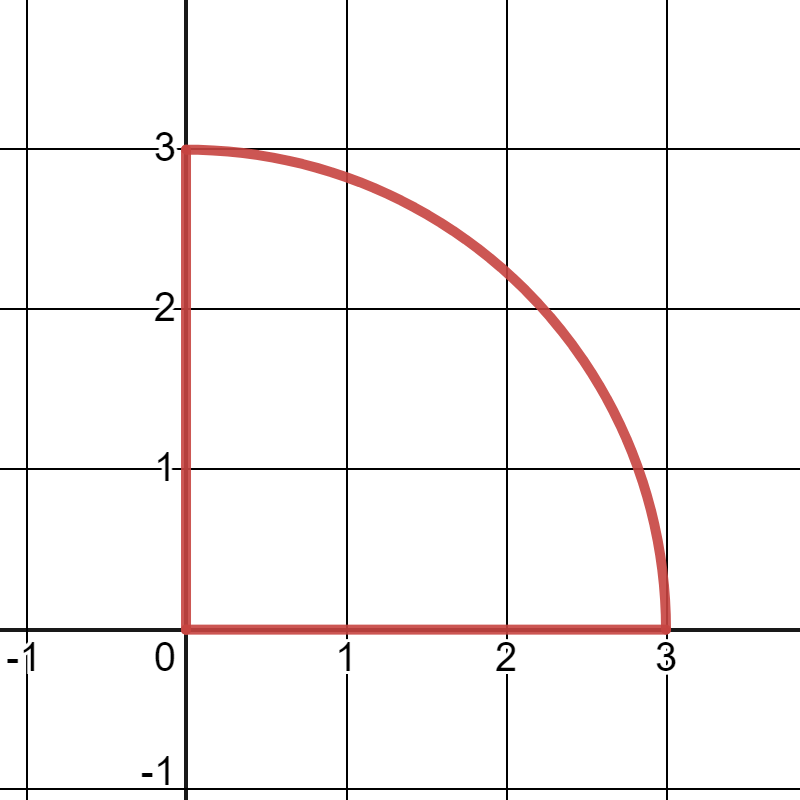
\includegraphics[scale=0.2]{Figures/521}\\Quarter Disc of Radius 3.
\end{center}
\vspace{1em}

Imagine that we want to integrate $f(x,y)=1+x+2y$ over $R$. That is, we want to find $$\iint_R 1+x+2y\ dA. $$ This is certainly possible, but quite annoying. So instead, we might think that while describing a circle in rectangular coordinates is tedious, this region is incredibly simple to describe in polar coordinates! That is, if we were to use the change of variables $x=r\cos\theta$ and $y=r\sin\theta$, then we get that our region is just 
$$R=\left\{(r,\theta): \ 0\leq\theta\leq \frac{\pi}{2},\ 0\leq r\leq 3 \right\}$$ 
and our function changes to 
$$f_t(r,\theta)=1+r\cos\theta+2r\sin\theta.$$ 
The double integral itself has no idea what polar coordinates are. So integrating 
$$\int_{0}^{3}\int_{0}^{\pi/2}1+r\cos\theta+2r\sin\theta\ d\theta \ dr $$ 
is just a double integral over a rectangular region, complete with being able to commute our integrals! In fact, that rectangular region just looks like this!

\vspace{1em}
\begin{center}
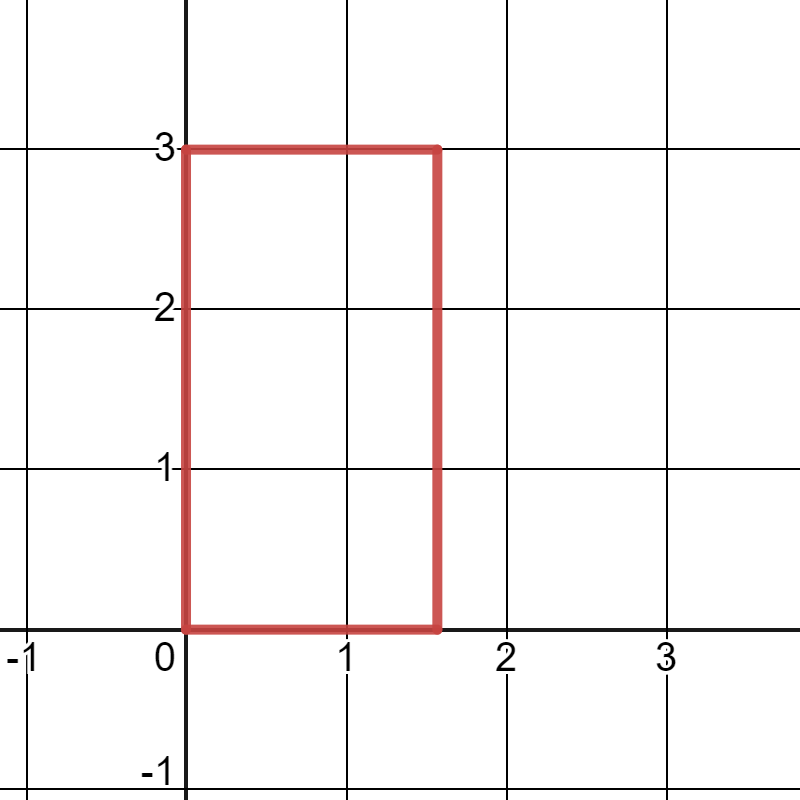
\includegraphics[scale=0.2]{Figures/522}\\$R$ in ``Polar'' Coordinates.
\end{center}
\vspace{1em}

Note also that our new surface, $$f_t(r,\theta)=1+r\cos\theta+2r\sin\theta\ $$ is much harder to describe, but still has the correct height above corresponding sections of $R$. That is, we can take any $(x,y)$ point in $R$ like $(\sqrt{2},\sqrt{2})$, then plug that into $f(x,y)$ to get 
$$f(\sqrt{2},\sqrt{2})=1+\sqrt{2}+2\sqrt{2}=1+3\sqrt{2}. $$ 
Then, we take that same point point, convert it to polar coordinates, 
$$(\sqrt{2},\sqrt{2})\to\left(2,\frac{\pi}{4}\right) $$ 
and when we plug that into $f_t(r,\theta)$, we get the same result, 

\begin{align*}
f_t\left(2,\frac{\pi}{4}\right)=&1+2\cos\left(\frac{\pi}{4}\right)+2\left(2\sin\left(\frac{\pi}{4}\right)\right)\\
=&1+2\left(\frac{\sqrt{2}}{2}\right)+4\left(\frac{\sqrt{2}}{2}\right)\\
=&1+\sqrt{2}+2\sqrt{2}\\
=&1+3\sqrt{2}.
\end{align*}

However, when we integrate, we get two different results:

\begin{align*}
\int_{0}^{3}\int_{0}^{\sqrt{1-x^2}} 1+x+2y\ dy\ dx=&27+\frac{9\pi}{4}\approx34.069\\
\int_{0}^{3}\int_{0}^{\pi/2}1+r\cos\theta+2r\sin\theta\ d\theta \ dr=&\frac{27}{2}+\frac{3\pi}{2}\approx18.212.
\end{align*}

This makes sense! After all, these regions have two different areas. Our original $R$ has an area of $\frac{9\pi}{4} $ and the polar version has an area of $\frac{3\pi}{2}$, so the original version is $1.5$ times larger than the polar version. But just multiplying by $1.5$ doesn't fix the problem, so what's going on here?

\vspace{1em}

The problem is that when we convert to polar coordinates, while we are scaling the region, we are not scaling every part of the region at the same rate. For example, consider the two subregions of $R$ below.

\vspace{1em}
\begin{center}
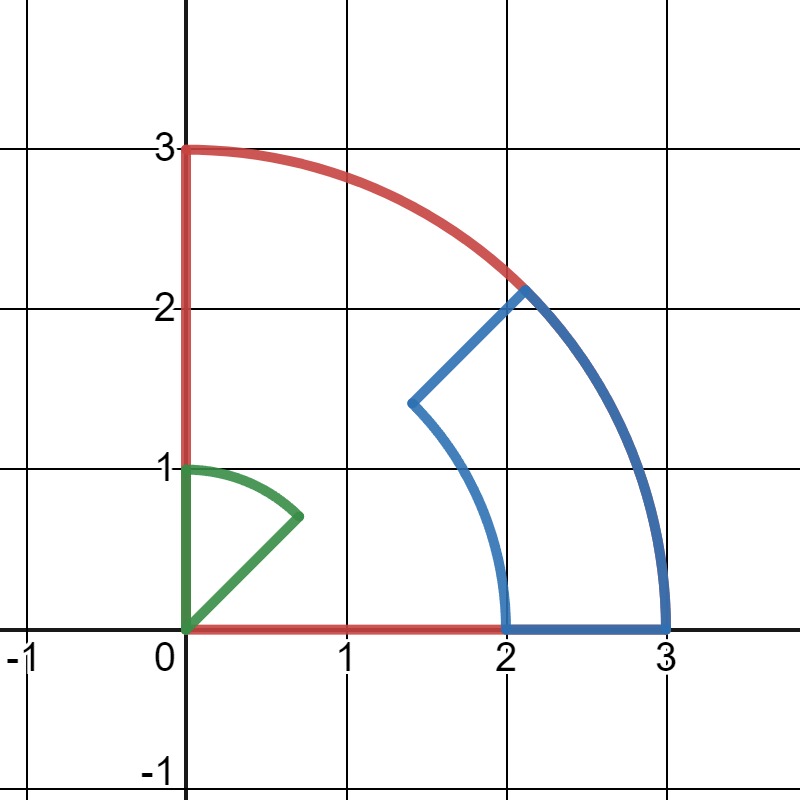
\includegraphics[scale=0.2]{Figures/523}\qquad 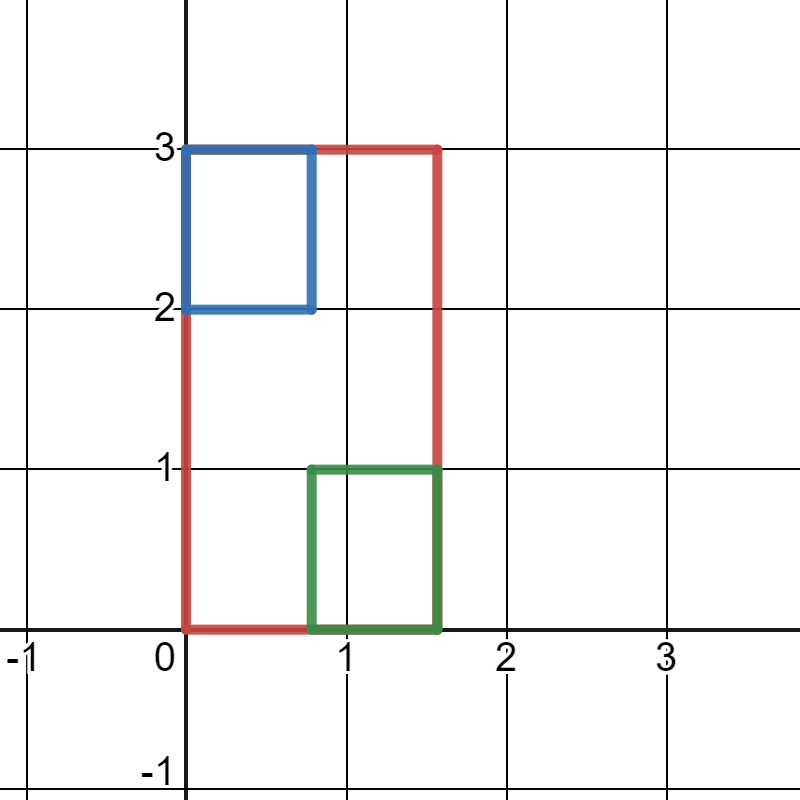
\includegraphics[scale=0.2]{Figures/524}\\Sub-regions of $R$ in Rectangular and Polar Coordinates.
\end{center}
\vspace{1em}

In both of the above graphs, the blue sub-region can be described by the polar coordinates 
$$R_b=\left\{(r,\theta): \ 0\leq\theta\leq \frac{\pi}{4},\ 2\leq r\leq 3 \right\}$$ 
and the green sub-region can be described by the polar coordinates
$$R_g=\left\{(r,\theta): \ \frac{\pi}{4}\leq\theta\leq \frac{\pi}{2},\ 0\leq r\leq 1 \right\}$$ 
In the left image, which is before the polar transformation, the blue sub-region is clearly \textit{larger} than the green one, while in the right image, after the polar transformation, the two regions are the same exact size! This transformation is scaling different parts of this region by different amounts. So we need some way of re-scaling the region after the transformation to ensure that our integrals match up. That scaling factor depends on the \textbf{Jacobian.}
\end{example}

So what is this magical Jacobian? Well, it's a matrix, so that's fun. In Linear Algebra, we write transformations between two different coordinate systems (or vector spaces) as matrix multiplication. Well, we specifically refer to \textit{linear} transformations as matrix multiplication, and of course, our problem is that often times the transformations we want to use here are often \textit{not} linear. The Jacobian is the matrix that gives a linear approximation of our non-linear transformations. Of course, how do we do linear approximations? You guessed it, lots of derivatives! The Jacobian essentially collects all the partial derivatives of each function in our transformation and stores them in a matrix.

\begin{definition}{Jacobian}
Let $\vcf$ be a function $\vcf: \bbr^n\to\bbr^n$. That is, $\vcf$ is a transformation between 2 $n$-dimensional vector spaces, or $$\vcf=\bmat{f_1(x_1,x_2,\ldots,x_n)\\ f_2(x_1,x_2,\ldots,x_n)\\ \vdots \\  f_n(x_1,x_2,\ldots,x_n)}. $$ Then the \textbf{Jacobian} of $\vcf$ is the matrix
$$J=\bmat{\frac{\del \vcf}{\del x_1} & \frac{\del \vcf}{\del x_2} & \cdots & \frac{\del \vcf}{\del x_n}}=\bmat{(\nabla f_1)^T\\(\nabla f_2)^T\\ \vdots\\ (\nabla f_n)^T}=
\bmat{
\frac{\del f_1}{\del x_1} & \cdots & \frac{\del f_1}{\del x_n} \\
\vdots  & \ddots & \vdots \\
\frac{\del f_n}{\del x_1} & \cdots & \frac{\del f_n}{\del x_n}
}$$ where $(\nabla f_i)^T$ is the transpose (to a row vector) of the gradient of $f_i$.

\vspace{1em}

In particular, for a $2$-dimensional change of coordinates, $x=x(u,v)$ and $y=y(u,v)$, the Jacobian is $$J=\bmat{\frac{\del x}{\del u} & \frac{\del x}{\del v} \\ \frac{\del y}{\del u} & \frac{\del y}{\del v}}=\bmat{x_u & x_v \\ y_u & y_v}.$$ For a $3$-dimensional change of coordinates, $x=x(u,v,w)$, $y=y(u,v,w)$ and $z=z(u,v,w)$, then the Jacobian is $$J=
\bmat{
\frac{\del x}{\del u} & \frac{\del x}{\del v} & \frac{\del x}{\del w}\\
\frac{\del y}{\del u} & \frac{\del y}{\del u} & \frac{\del y}{\del w}\\
\frac{\del z}{\del u} & \frac{\del z}{\del v} & \frac{\del z}{\del w}
}=\bmat{x_u & x_v & x_w \\ y_u & y_v & y_w \\ z_u & z_v & z_w}.$$
\end{definition}

What we really want, actually, to complete our transformations and to be able to integrate according to our new variables, is the \textbf{determinant} of the Jacobian. \hyperlink{det}{We first did determinants way back when we covered the cross product.} So how do these pieces come together? Well, the determinant of the Jacobian, $\det(J)$, tells us what non-linear scaling factor we need to apply to make our integrals before and after the transformation the same!

\begin{claim}{Change of Variables, Double Integral}
Consider the surface $f(x,y)$ over the region $R$. When applying the transformation $x=x(u,v)$, $y=y(u,v)$, the region becomes $S$, the function transforms to $f_t(u,v)$ and $$\iint_R f(x,y)\ dA=\iint_S f_t(u,v)\cdot |\det(J)|\ d\ca{A} $$ where $d\ca{A}$ indicates that the variables of integration are now $u$ and $v$ instead of $x$ and $y$ and $|\det(J)|$ is the absolute value of the determinant of the Jacobian of the transformation.
\end{claim}

\begin{claim}{Change of Variables, Triple Integral}
Consider the function $f(x,y,z)$ over the region $R$. When applying the transformation $x=x(u,v,w),$ $y=y(u,v,w)$ and $z=z(u,v,w)$, the region becomes $S$, the function transforms to $f_t(u,v,w)$ and $$\iiint_R f(x,y,z)\ dV=\iiint_S f_t(u,v,w)\cdot |\det(J)| \ d\ca{V} $$ where $d\ca(V)$ indicates that the variables of integration are now $u$, $v$ and $w$ instead of $x$, $y$ and $z$ and $|\det(J)|$ is the absolute value of the determinant of the Jacobian of the transformation.
\end{claim}

Lets use this to compute the Jacobians and their determinants in general for transformations for double and triple integrals!

\begin{exercise}{Jacobian Determinants}
\begin{enumerate}
\item Consider the transformation $x=x(u,v)$ and $y=y(u,v)$. Compute $\det(J)$, the determinant of the Jacobian of a 2-dimensional transformation. 
\vspace{1em}
\item Consider the transformation $x=x(u,v,w)$, $y=y(u,v,w)$ and $z=z(u,v,w)$. Compute $\det(J)$, the determinant of the Jacobian of a 3-dimensional transformation.
\end{enumerate}
\end{exercise}

\begin{exercise}{The Transformation from Before!}
Consider the region $R$ that is the triangle with vertices at $(0,0)$, $(1,2)$ and $(2,1)$. This is the region bounded by the lines. You used the transformation $x(u,v)=u+v$ and $y(u,v)=u-v$ to transform this region before. Now find the Jacobian and $|\det(J)|$ for this transformation. Then use this transformation to evaluate the integral: $$\iint_R 2xy \ dA.$$ 
\end{exercise}

Now we can refer back to our example!

\begin{example}{A Less Annoying Example}
Lets return to the beginning-- the volume beneath the surface $f(x,y)=1$ where $D$ is the disk of radius 1. But lets convert to polar coordinates. That is, convert from variables $(x,y)$ to variables $(r,\theta)$. Then $x=x(r,\theta)=r\cos\theta$ and $y=y(r,\theta)=r\sin\theta$. We need to do a few tasks:
\vspace{1em}
\begin{itemize}
\item Convert our bounds: The disk of radius 1 in polar coordinates is $$S=\big\{(r,\theta):\ 0\leq r\leq 1,\ 0\leq\theta\leq 2\pi \big\}.$$
\vspace{1em}
\item Convert our function: Since $f(x,y)=1$, $f_t(r,\theta)=1$ also.
\vspace{1em}
\item Compute our Jacobian and its determinant: 
\begin{align*}J=&\bmat{x_r & x_\theta\\y_r&y_\theta} \\
=&\bmat{\frac{\del}{\del r}(r\cos\theta)& \frac{\del}{\del \theta}(r\cos\theta)\\ \frac{\del}{\del r}(r\sin\theta)& \frac{\del}{\del \theta}(r\sin\theta)}\\
=&\bmat{\cos\theta & -r\sin\theta\\ \sin\theta & r\cos\theta}.
\end{align*}
Then the determinant:
\begin{align*}
\det(J)=&\vmat{\cos\theta & -r\sin\theta\\ \sin\theta & r\cos\theta}\\
=& (\cos\theta)(r\cos\theta)-(-r\sin\theta)(\sin\theta)\\
=& r\cos^2\theta+r\sin^2\theta\\
=&r(\cos^2\theta+\sin^2\theta)\\
=&r.
\end{align*}
\end{itemize}
Then we can rewrite our integral:
$$\iint_D 1 \ dA=\iint_S 1 |r| \ d\ca{A}=\int_{0}^{2\pi}\int_{0}^1 r \ dr \ d\theta.$$
Then we need only evaluate the iterated integral.

\begin{align*}
\int_{0}^{2\pi}\int_{0}^1 r \ dr \ d\theta=& \int_{0}^{2\pi}\Bigg[\frac{r^2}{2} \Bigg]_{r=0}^{r=1} \ d\theta\\
=&\int_0^{2\pi}\frac{1}{2} \ d\theta \\
=&\Bigg[\frac{\theta}{2} \Bigg]_{\theta=0}^{\theta=2\pi} \\
=&\pi.
\end{align*}

\end{example}

\begin{exercise}{Changing Coordinates}
Let $R$ be the diamond shaped region with vertices at $(0,0)$, $(5/2,5/2)$, $(5,0)$ and $(5/2,-5/2)$. Evaluate the integral using the transformation $x(u,v)=2u+3v$, $y(u,v)=2u-3v$. $$\iint_R x+y \ dA .$$ 
Hint: Draw a graph of the region before the transformation. What are the equations of the lines that bound the diamond shape? What happens to the equations of those lines when you apply the desired transformation?
\end{exercise}

\begin{exercise}{U-Substitution and the Jacobian}
Consider the integral $$\int_{0}^1 x\sqrt{1+x^2} \ dx.$$
Traditionally, we would solve this integral using the $u$-substitution, $u=1+x^2$. Instead, consider the change of variables $x(u)=\sqrt{u-1}$, and compute the integral using our change of variables formula. Note that if our Jacobian is a $1\times 1$ matrix, like $$J=\bmat{j_1}, $$ then $\det(J)=j_1$.
\end{exercise}
\subsection{Common Changes of Variables: Polar, Cylindrical, Spherical.}

There are a few very common transformations, and their Jacobians are worth paying special note to. One is the polar transformation for double integrals that we just saw.

\begin{claim}{Polar Jacobian}
Let $f(x,y)$ be a function over the region $R$, subject to the transformation
\begin{align*}
x(r,\theta)=&r\cos\theta\\
y(r,\theta)=&r\sin\theta.
\end{align*}
Then $\det(J)=r$ so $$\iint_R f(x,y)\ dA=\iint_S f_t(r,\theta)\cdot r\ d\ca{A}.$$
\end{claim}

\begin{exercise}{Polar Integration}
Let $D$ be the region between the circles of radius 2 and radius 5 centered at the origin that lies in the first quadrant. Evaluate $$\iint_D 2xy\ dA. $$
\end{exercise}

\begin{exercise}{Calculus II Formula for Polar Area}
Note that in general, for a given region $R$, $$\iint_R 1\ dA $$ computes the area of that region. Recall from Calculus II that $$\int_{\alpha}^{\beta}\frac{\big(r(\theta)\big)^2}{2}\ d\theta $$ gives the area between $r(\theta)$ and the origin between the angles $\alpha$ and $\beta$. 

\vspace{1em}

Let $R$ be the region where $0\leq r\leq r(\theta)$ and $\alpha \leq \theta\leq \beta$. Show that by converting to polar coordinates and evaluating the inner integral, $$\iint_R 1\ dA$$ gives the Calculus II formula for polar area.
\end{exercise}

\begin{exercise}{A White Whale}
An integral of considerable importance is $$\int_{-\infty}^{\infty}e^{-x^2}\ dx.$$ The function $e^{-x^2} $ is the basis of the normal distribution\footnote{Actually statistics uses $e^{-\frac{1}{2}x^2} $ rather than $e^{-x^2}$ because the extra constant factor makes variance come out nicer, but the logic here still holds without the extra constant.}, a very important idea in statistics. 

\vspace{1em}
\begin{center}
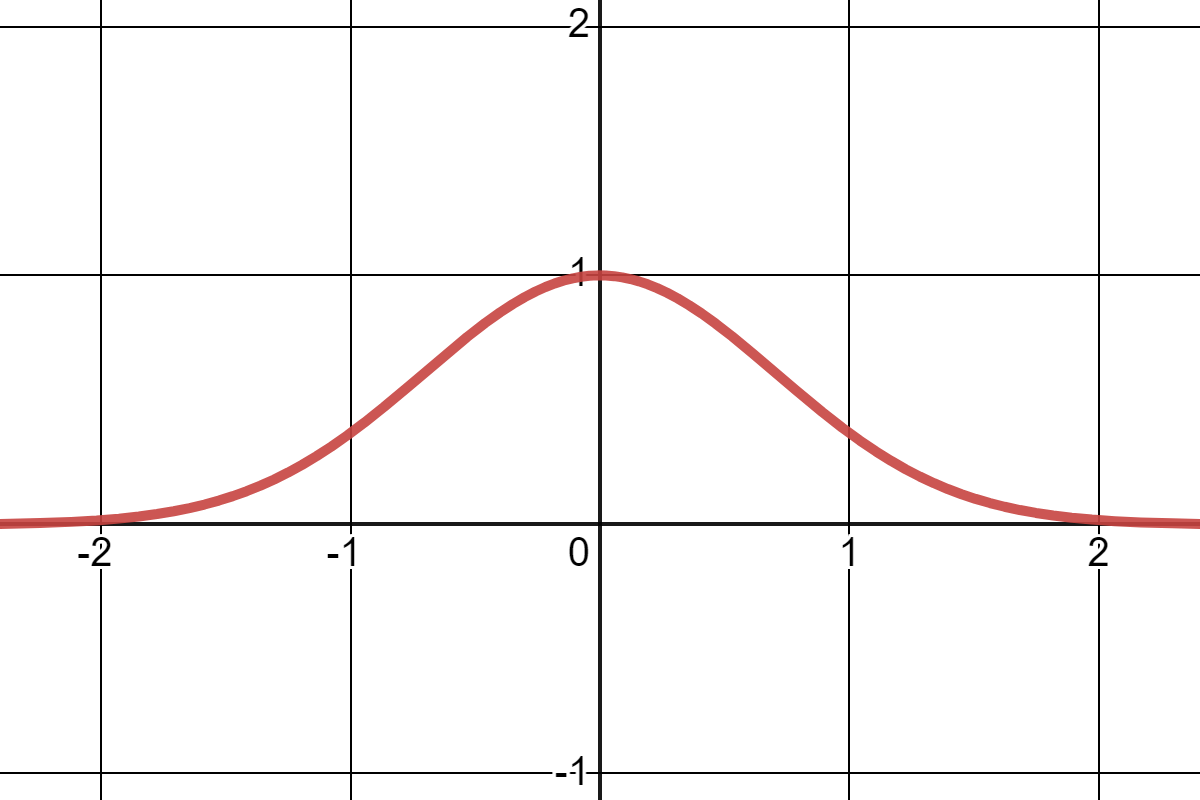
\includegraphics[scale=0.2]{Figures/531}\\ The graph of the function $e^{-x^2}$.
\end{center}
\vspace{1em}

In statistics, it is common practice to standardize distributions, so it is desired that we find some constant $c$ such that the area beneath $ce^{-x^2}$ is exactly 1. To do that, we need to be able to evaluate the integral above. There's just one problem-- which is that you can't find a closed form antiderivative for $e^{-x^2}$. 

\vspace{1em}

So what can we do? Let's let $$C=\int_{-\infty}^{\infty}e^{-x^2}\ dx.$$ Then let's consider instead a $3$-dimensional version of this integral, $$\iint_R e^{-x^2-y^2}\ dA $$ where $R=[-\infty,\infty]\times[-\infty,\infty].$ 

\vspace{1em}
\begin{center}
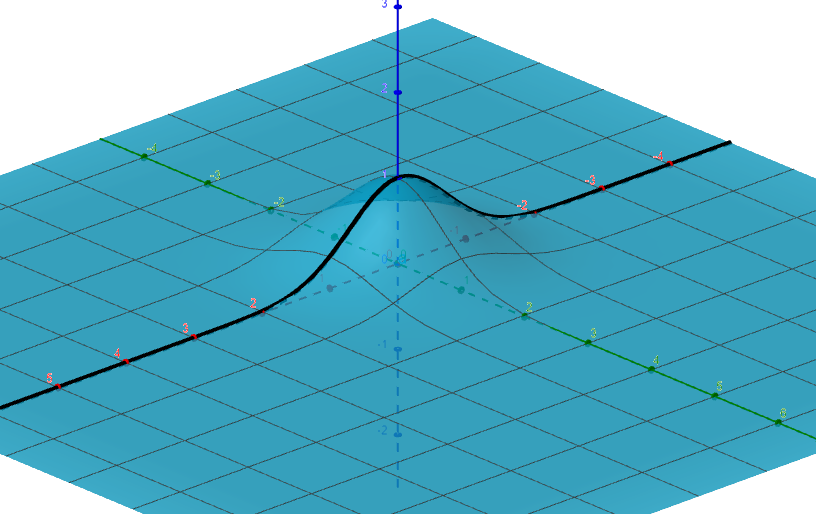
\includegraphics[scale=0.5]{Figures/532}\\ Click this \href{https://www.geogebra.org/3d/yrkngady}{geogebra link} for an interactive version of this graph.
\end{center}
\vspace{1em}
Consider the cross sectional area beneath the black curve in the graph above. The black curve is the portion of the surface that intersects the plane $y=0$. The area beneath that curve should be exactly $C$, or the value of the integral $$\int_{-\infty}^{\infty}e^{-x^2}\ dx.$$
If we move the line a little (which you can do in the interactive graph by using the slider), then you might notice that the new curve is the same curve as before, just scaled by some factor in the vertical direction. That is, the curve formed from the intersection of $y=c$ and $e^{-x^2-y^2}$ is a constant multiple of $e^{-x^2}$, and so it's area is some multiple of the unknown $C$ that we're looking for. In fact, the area of each cross section is just $C\cdot e^{-y^2}.$ We can reach back to Calculus II and compute the volume of this object using cross sectional areas as $$V=\int_{-\infty}^{\infty}C\cdot e^{-y^2}\ dy. $$ Since $C$ is a constant, we can factor it out of the integral as $$V=C\int_{-\infty}^{\infty}e^{-y^2}\ dy .$$ But remember that $$C=\int_{-\infty}^{\infty}e^{-x^2}\ dx=\int_{-\infty}^{\infty}e^{-y^2}\ dy.$$ So the volume beneath this surface is just $V=C^2$. \footnote{If you're having a hard time with the argument that $$\iint_R e^{-x^2-y^2}\ dA=\left(\int_{-\infty}^{\infty}e^{-x^2}\ dx\right)^2, $$ there is an excellent \href{https://youtu.be/cy8r7WSuT1I?t=551}{video from 3blue1brown} on the topic. He approaches the integral that we want to solve in a slightly more roundabout way that is accessible without double integration, but the visuals are excellent. The argument in question begins at about 9:11 in the video.}

\vspace{1em}

Great. So now we know that $$C^2=\iint_R e^{-x^2-y^2}\ dA $$ where $R=[-\infty,\infty]\times[-\infty,\infty].$ Now all that remains is to calculate that integral. Use a polar transformation to compute the integral and then give the value of $C$.

\end{exercise}

\hypertarget{cylind}{Another common transformation is the triple integral in cylindrical coordinates.}

\begin{exercise}{Cylindrical Jacobian}
Cylindrical coordinates in 3-space are much like polar coordinates in 2-space. To convert to cylindrical coordinates, you'll use the transformation:
\begin{align*}
x(r,\theta,z)=&r\cos\theta\\
y(r,\theta,z)=&r\sin\theta\\
z(r,\theta,z)=&z.
\end{align*}
Find the Jacobian and show that $|\det(J)|=r$ for this transformation.
\end{exercise}

\begin{exercise}{Cylindrical Integration}
Let $D$ be the region that lies below the plane $z=x+2$ and above the $xy$-plane and between the cylinders $x^2+y^2=1$ and $x^2+y^2=4$. Use a change to cylindrical coordinates to evaluate $$\iiint_D y\ dV. $$
\end{exercise}

\hypertarget{spherical}{A third common transformation is the triple integral in spherical coordinates}. Spherical coordinates have a few different methods of computing-- here we use the typical mathematical convention where $\theta$ refers to the \textit{azimuthal angle} and $\phi$ refers to the \textit{polar angle}. That is, $\theta$ is the angle in standard position in the $xy$-plane, and $\phi$ is the angle from the positive $z$-axis to the point. Either way, we use $\rho$ to denote the spherical radius (i.e. the distance from the point to the origin). That is, $\rho,$ $ \theta$ and $\phi$ are as below:

\begin{center}%UPDATE DIAGRAM
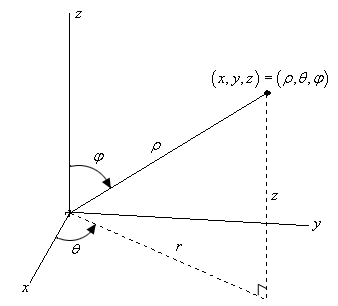
\includegraphics[scale=0.5]{Figures/sphericalcoord}
\end{center}

Note that many sources (usually physics sources) switch $\theta$ and $\phi$. For example, if you go to the \href{}{Wikipedia page on the Spherical coordinate system}, you can see that they use the convention that $\theta$ is the polar angle and $\phi$ is the azimuthal angle. They also use $r$ for the spherical radius. While the physics convention has an ISO standard on its side, I argue that it is more correct to use a consistent $\theta$ between polar, cylindrical and spherical coordinates, and similarly think that we should not use $r$ for the spherical radius as it differs from the polar and cylindrical radius.

\begin{exercise}{Spherical Jacobian}
Spherical coordinates are another analogue to polar coordinates in 2-space, but utilize a radius and two angles. To convert to spherical coordinates, you'll use the transformation:
\begin{align*}
x(\rho,\phi,\theta)=&\rho\sin\phi\cos\theta\\
y(\rho,\phi,\theta)=&\rho\sin\phi\sin\theta\\
z(\rho,\phi,\theta)=&\rho\cos\phi.
\end{align*}
Find the Jacobian and show $|\det(J)|=\rho^2\sin\phi$ for this transformation.
\end{exercise}

\begin{exercise}{Spherical Integration}
Let $D$ be the region between the upper half of the sphere $x^2+y^2+z^2=1$ and the $xy$-plane. Evaluate $$\iiint_D 16x\ dV. $$
\end{exercise}

\subsection{Application: Surface Area}
What can we use multiple integrals for? Well, there are direct applications in fields like statistics. Where something like the normal distribution calculates probability as an integral as the area beneath a probability function, for a multivariate probability, you would use multiple integrals! The two applications we will cover are \textit{surface area} and \textit{center of mass}.

First, surface area. Surface area is computed with regards to a double integral in much the same way that \textit{arc length} is computed with respect to a single integral. Recall that the arc length of the function $f$ from $x=a$ to $x=b$ is computed as:
$$\ell=\int_a^b \sqrt{1+(f')^2}\ dx. $$
So then to compute the surface area, we use the following.

\begin{definition}{\hypertarget{surfarea}{Surface Area}}
The area of the surface $f(x,y)$ above the region $R$ in the $xy$-plane is $$S=\iint_R \sqrt{1+(f_x)^2+(f_y)^2}\ dA. $$
\end{definition}

Lets try it.

\begin{example}{Surface Area}
Let's find the surface area of the part of the plane $x+2y+z=4$ that lies in the first octant. First, we'll need to rewrite our plane as some function of $x$ and $y$. This is relatively simple, and we get the function $$f(x,y)=4-x-2y. $$
Next, lets figure out our bounds. You can see a graph of this plane in Geogebra 3d \href{https://www.geogebra.org/3d/qevz8eev}{here}. The first octant is the area above the first quadrant in the $xy$ plane. To find our bounds then, we need to figure out where the function intersects the $xy$-plane, which is as straightforwards as letting $z=0$. In this case, we get that $x+2y=4$, which if we solve for $x$ we get $x=4-2y$. Then we can select our bounds:
\begin{align*}
0\leq x&\leq 4-2y \\
0\leq y&\leq 2.
\end{align*}
Now we return to $f(x,y)$. We need our partials for the surface area formula:
\begin{align*}
f_x=&-1\\
f_y=&-2
\end{align*}
Then our surface area integral is:
\begin{align*}
S=&\iint_R \sqrt{1+(f_x)^2+(f_y)^2}\ dA\\
=&\int_{0}^2 \int_{0}^{4-2y}\sqrt{1+(-1)^2+(-2)^2}\ dx \ dy \\
=&\int_{0}^2 \int_{0}^{4-2y}\sqrt{6}\ dx \ dy.
\end{align*}
Computing that integral:
\begin{align*}
\int_{0}^2 \int_{0}^{4-2y}\sqrt{6}\ dx \ dy =& \int_{0}^2\Bigg[\sqrt{6}\Bigg]_{x=0}^{x=4-2y}\ dy\\
=&\int_0^2 \sqrt{6}(4-2y) \ dy\\
=&\sqrt{6}\int_0^2 4-2y\ dy\\
=&\sqrt{6}\Bigg[4y-y^2 \Bigg]_{y=0}^{y=2}\\
=&\sqrt{6}(8-4)\\
=&4\sqrt{6}.
\end{align*}
\end{example}

\begin{pexercise}{Surface Area}
Find the area of the surface $f(x,y)=3+2y+\frac{1}{4}x^4$ that lies above the region $R=\{(x,y):\ 0\leq x\leq 1,\ 0\leq y\leq x^5 \}$.
\end{pexercise}

\begin{exercise}{Surface Area of a Sphere}
Find the surface area of a sphere with radius 1 using multiple integration. Hint: Note that the top half of a sphere with radius 1 is $f(x,y)=\sqrt{1-x^2-y^2}$. Take your partials, set up your integral as $$ S=2\iint_R \sqrt{1+(f_x)^2+(f_y)^2} \ dA,$$ then convert \textit{that} to polar coordinates!
\end{exercise}

\subsection{Application: Center of Mass}

Our other application that we want to cover is an application of both double and triple integration: center of mass. In Calculus II, you saw how to compute center of mass of a two dimensional object with constant density. Here, we consider objects with variable density in 1, 2 and 3 dimensions.

First, however, we should consider a relatively easy physics problem. 

\begin{example}{Give me a long enough lever}
Suppose we have a 4000 kilogram elephant positioned 3 meters from the fulcrum of a seesaw. How far away from the fulcrum must an 80kg person stand in order to balance the seesaw?

In order for the seesaw to be balanced, the torque on both sides must be the same. We'll ignore the mass of the seesaw for simplicity. Torque is rotational force, and is computed as $\tau=f\cdot d$, where $f$ is the force applied and $d$ is the distance from the fulcrum. In this situation our force is from gravity, so we get $f=gm$. Then our elephant torque is \begin{align*}\tau_1=&gm_1 x_1\\=&g(4000)(3)\\=&12000g.\end{align*} and the person's torque is \begin{align*}\tau_2=gm_2x_2\\=&g(80)x_2.\end{align*}
When we set these equal to each other, we find that $$12000g=80gx_2.$$ We quickly find that $x_2=150$. So our 80kg human should stand 150m away from the fulcrum to lift the elephant.
\end{example}

Let's generalize.

\begin{exercise}{Generalizing}
Lets say that we have two objects on a line of negligible mass. Object 1 has a mass of $m_1$ and is at the coordinate $x_1$. Object 2 has a mass of $m_2$ and is at $x_2$. Let the center of mass be at the unknown coordinate $\overline{x}$. Then if the objects are balanced at the center of mass, their torques must be equal and opposite. That is: $$m_1(x_1-\overline{x})-m_2(x_2-\overline{x})=0. $$
Solve the above formula for $\overline{x}$ to show that $$\overline{x}=\frac{m_1x_1+m_2x_2}{m_1+m_2}.$$
\end{exercise}

Note: We call the quantities $m_1x_1$ and $m_2x_2$ the \textit{moments} of the two objects respectively. So then the coordinate of the center of gravity is the sum of the moments divided by the sum of the masses (or the total mass). This yields the even more generalized formula for the center of mass of $n$ objects on the $x$-axis:
$$\overline{x}=\frac{\sum_{k=1}^{n}m_kx_k }{\sum_{k=1}^{n}m_k}.$$

\begin{exercise}{More Discrete Objects}
Suppose that we have 4 objects on the $x$-axis. Object 1 is at $x=-2$ and has mass $3$kg. Object 2 is at $x=2$ and has mass $5$kg. Object 3 is at $x=-5$ and has mass $2$kg. Object 4 is at $x=7$ and has mass $1$kg. Find the center of gravity of the system.
\end{exercise}

We can continue to generalize even further. Rather than $n$ discrete objects, we can take a $1$-dimensional object with some continuous density function $\rho(x) $. Then, we get:

\begin{definition}{1-Dimensional Center of Mass}
Let $\rho(x)$ be an integrable density function over the integral $[a,b]$ which represents a rod of variable density. Then the center of mass is located at the point $\overline{x}=\frac{M}{m}$, where $M$ is the total moment and $m$ is the total mass of the object, which can be calculated as:
$$M=\int_a^b x\rho(x)\ dx\text{ and }m=\int_a^{b}\rho(x)\ dx.$$
\end{definition}

Note 1: Notice the similarity between the discrete case, where $$\overline{x}=\frac{\displaystyle\sum_{k=1}^{n}m_kx_k }{\displaystyle\sum_{k=1}^{n}m_k} $$ and the continuous case where $$\overline{x}=\frac{\displaystyle\int_{a}^b x\rho(x)\ dx}{\displaystyle\int_a^b\rho(x)\ dx}. $$
Note 2: The center of mass formulas you saw in Calculus II are simply taking a 2-dimensional object of uniform density and reducing it to a 1-dimensional object where the density is given at a single point as the width of that object at that point. You do this in the $x$-direction and the $y$-direction and end up with your two coordinates!

Now lets take this same idea and bring it into higher dimensional objects.

\begin{definition}{2-Dimensional Center of Mass}
Consider a 2-dimensional region $R$ with density function $\rho(x,y)$ which is integrable over all of $R$. Then the center of mass of the region is $(\overline{x},\overline{y})$ where $$\overline{x}=\frac{1}{m}\iint_R x\cdot\rho(x,y) \ dA $$ and $$\overline{y}=\frac{1}{m}\iint_R y\cdot\rho(x,y)\ dA.$$
As before, the mass of the object, $m$ is $$m=\iint_R \rho(x,y)\ dA. $$
\end{definition}

\begin{exercise}{The Cosine Gumdrop Revisited}
Consider the shape between $y=\cos(x)$ and the $x$-axis with constant density $\rho(x,y)=1$. Find the center of gravity of this gumdrop shape using double integrals. Hint: Save some time by using symmetry!
\end{exercise}

\begin{exercise}{Variable Density}
Consider a rectangular plate with opposite corners at $(0,0)$ and $(2,1)$, with density $\rho(x,y)=3-x$ (the plate is densest towards the $y$-axis and gets less dense as you move to the right). Find the center of gravity of the plate.
\end{exercise}

And of course, we can generalize yet again to three dimensional objects.

\begin{definition}{3-Dimensional Center of Mass}
Consider a 3-dimensional region $R$ with density function $\rho(x,y,z)$ which is integrable over all of $R$. Then the center of mass of the region is $(\overline{x},\overline{y},\overline{z})$, where
 \begin{align*}
 \overline{x}=&\frac{1}{m}\iiint_R x\cdot\rho(x,y,z) \ dV \\
 \overline{y}=&\frac{1}{m}\iiint_R y\cdot\rho(x,y,z)\ dV \\
 \overline{z}=&\frac{1}{m}\iiint_R z\cdot\rho(x,y,z)\ dV
 \end{align*}
 and $$m=\iiint_R \rho(x,y,z)\ dV. $$
\end{definition}

\begin{exercise}{3-Dimensional, Constant Density}
Use triple integrals to find the center of gravity of the upper half sphere of radius 1 with constant unit density. Hint: You'll almost definitely want to use a change to polar coordinates for this. 
\end{exercise}
\renewcommand\thesubsection{\thesection.\Alph{subsection}}
\setcounter{subsection}{18}
\subsection{Multiple Integrals Summary}
\begin{theorem}{Fubini's Theorem for Evaluating Double Integrals}
Let $f(x,y)$ be continuous on the rectangle $R=[a,b]\times[c,d]$. Then $$\iint_R f(x,y)\ dA=\int_{a}^{b}\int_{c}^{d}f(x,y)\ dy\ dx=\int_{c}^{d}\int_{a}^{b}f(x,y)\ dx\ dy.$$ In other words, we can compute the double integral through iterated integration with respect to $x$ then with respect to $y$.
\end{theorem}

\begin{definition}{Non-Rectangular Double Integrals}
\begin{itemize}
\item Let $f(x,y)$ be continuous on the domain $D=\{(x,y):\ a<x<b,\ g(x)<y<h(x) \}.$ Then: $$\iint_D f(x,y)\ dA=\int_{a}^{b}\int_{g(x)}^{h(x)}f(x,y)\ dy \ dx. $$
\item Let $f(x,y)$ be continuous on the domain $D=\{(x,y):\ g(y)<x<h(y).\ a<y<b \}. $ Then: $$\iint_{D}f(x,y)\ dA=\int_{a}^b\int_{g(y)}^{h(y)}f(x,y)\ dx \ dy. $$
\end{itemize}
\end{definition}

\begin{definition}{Triple Integral on a Rectangular Prism}
Let $f(x,y,z)$ be a function and $R$ be the rectangular prism $R=[a,b]\times[c,d]\times[e,f]$. Then we can evaluate the triple integral $$\iiint_R f(x,y,z)\ dV=\int_e^f\int_c^d\int_a^b f(x,y,z) \ dx \ dy \ dz.$$
You can also order the integration any of the 6 possible ways!
\end{definition}

\begin{definition}{Triple Integral on an Arbitrary Region}
Let $f(x,y,z)$ be a function and $D$ be a region in $3$-space such that $$D=\big\{(x,y,z): \ a\leq x\leq b,\ g(x)\leq y\leq h(x),\ G(x,y)\leq z\leq H(x,y)  \big\}.$$ Then the triple integral can be evaluated as the iterated integral: $$\iiint_D f(x,y,z)\ dV=\int_a^b\int_{g(x)}^{h(x)}\int_{G(x,y)}^{H(x,y)}f(x,y,z)\ dz \ dy \ dx. $$
\end{definition}

\begin{definition}{2-D Jacobian}
For a $2$-dimensional change of coordinates, $x=x(u,v)$ and $y=y(u,v)$, the Jacobian is $$J=\bmat{\frac{\del x}{\del u} & \frac{\del x}{\del v} \\ \frac{\del y}{\del u} & \frac{\del y}{\del v}}=\bmat{x_u & x_v \\ y_u & y_v}.$$
\end{definition}

\begin{definition}{3-D Jacobian}
For a $3$-dimensional change of coordinates, $x=x(u,v,w)$, $y=y(u,v,w)$ and $z=z(u,v,w)$, then the Jacobian is $$J=
\bmat{
\frac{\del x}{\del u} & \frac{\del x}{\del v} & \frac{\del x}{\del w}\\
\frac{\del y}{\del u} & \frac{\del y}{\del u} & \frac{\del y}{\del w}\\
\frac{\del z}{\del u} & \frac{\del z}{\del v} & \frac{\del z}{\del w}
}=\bmat{x_u & x_v & x_w \\ y_u & y_v & y_w \\ z_u & z_v & z_w}.$$
\end{definition}

\begin{claim}{Change of Variables, Double Integral}
Consider the surface $f(x,y)$ over the region $R$. When applying the transformation $x=x(u,v)$, $y=y(u,v)$, the region becomes $S$, the function transforms to $f_t(u,v)$ and $$\iint_R f(x,y)\ dA=\iint_S f_t(u,v)\cdot |\det(J)|\ d\ca{A} $$ where $d\ca{A}$ indicates that the variables of integration are now $u$ and $v$ instead of $x$ and $y$ and $|\det(J)|$ is the absolute value of the determinant of the Jacobian of the transformation.
\end{claim}

\begin{claim}{Change of Variables, Triple Integral}
Consider the function $f(x,y,z)$ over the region $R$. When applying the transformation $x=x(u,v,w),$ $y=y(u,v,w)$ and $z=z(u,v,w)$, the region becomes $S$, the function transforms to $f_t(u,v,w)$ and $$\iiint_R f(x,y,z)\ dV=\iiint_S f_t(u,v,w)\cdot |\det(J)| \ d\ca{V} $$ where $d\ca(V)$ indicates that the variables of integration are now $u$, $v$ and $w$ instead of $x$, $y$ and $z$ and $|\det(J)|$ is the absolute value of the determinant of the Jacobian of the transformation.
\end{claim}

\begin{definition}{Polar Transformation and Jacobian}
The polar transformation for a 2-dimensional function is given as 
\begin{align*}
x(r,\theta)=&r\cos\theta\\
y(r,\theta)=&r\sin\theta.
\end{align*}
The determinant of the Jacobian for the polar transformation is $$\det|J|=r. $$
\end{definition}

\begin{definition}{Cylindrical Transformation and Jacobian}
The cylindrical transformation for a 3-dimensional function is given as
\begin{align*}
x(r,\theta,z)=&r\cos\theta\\
y(r,\theta,z)=&r\sin\theta
z(r,\theta,z)=&z.
\end{align*}
The determinant of the Jacobian for the cylindrical transformation is $$\det|J|=r. $$
\end{definition}

\begin{definition}{Spherical Transformation and Jacobian}
The spherical transformation for a 3-dimensional function is given as 
\begin{align*}
x(\rho,\theta,\phi)=&\rho\sin\phi\cos\theta\\
y(\rho,\theta,\phi)=&\rho\sin\phi\sin\theta\\
z(\rho,\theta,\phi)=&\rho\cos\phi.
\end{align*}
The determinant of the Jacobian for the spherical transformation is $$\det|J|=\rho^2\sin\phi. $$
\end{definition}

\begin{definition}{Surface Area}
The area of the surface $f(x,y)$ above the region $R$ in the $xy$-plane is $$S=\iint_R \sqrt{1+(f_x)^2+(f_y)^2}\ dA. $$
\end{definition}

\begin{definition}{1-Dimensional Center of Mass}
Let $\rho(x)$ be an integrable density function over the integral $[a,b]$ which represents a rod of variable density. Then the center of mass is located at the point $\overline{x}=\frac{M}{m}$, where $M$ is the total moment and $m$ is the total mass of the object, which can be calculated as:
$$M=\int_a^b x\rho(x)\ dx\text{ and }m=\int_a^{b}\rho(x)\ dx.$$
\end{definition}

\begin{definition}{2-Dimensional Center of Mass}
Consider a 2-dimensional region $R$ with density function $\rho(x,y)$ which is integrable over all of $R$. Then the center of mass of the region is $(\overline{x},\overline{y})$ where $$\overline{x}=\frac{1}{m}\iint_R x\cdot\rho(x,y) \ dA $$ and $$\overline{y}=\frac{1}{m}\iint_R y\cdot\rho(x,y)\ dA.$$
As before, the mass of the object, $m$ is $$m=\iint_R \rho(x,y)\ dA. $$
\end{definition}

\begin{definition}{3-Dimensional Center of Mass}
Consider a 3-dimensional region $R$ with density function $\rho(x,y,z)$ which is integrable over all of $R$. Then the center of mass of the region is $(\overline{x},\overline{y},\overline{z})$, where
 \begin{align*}
 \overline{x}=&\frac{1}{m}\iiint_R x\cdot\rho(x,y,z) \ dV \\
 \overline{y}=&\frac{1}{m}\iiint_R y\cdot\rho(x,y,z)\ dV \\
 \overline{z}=&\frac{1}{m}\iiint_R z\cdot\rho(x,y,z)\ dV
 \end{align*}
 and $$m=\iiint_R \rho(x,y,z)\ dV. $$
\end{definition}

\subsubsection*{Companion Videos by Ken Monks}
\begin{itemize}
\item \href{https://www.youtube.com/watch?v=ga7g3kuoGBY}{Riemann Sum Definition of Double Integrals.}
\item \href{https://www.youtube.com/watch?v=14pepJeFyAQ}{Spherical Coordinates.}
\item \href{https://www.youtube.com/watch?v=6b6TWV9rFZM}{Triple Integrals in Spherical Coordinates.}
\end{itemize}

\renewcommand\thesubsection{\thesection.\arabic{subsection}}
\renewcommand\thesubsection{\thesection.\Alph{subsection}}
\setcounter{subsection}{17}
\subsection{Multiple Integrals Homework and Miscellaneous Practice}

\begin{pexercise}{Double Integral on Rectangle}
Let $R=[1,4]\times[0,3]$. Evaluate $$\iint_R 6y\sqrt{x}-2y^3 \ dA .$$
\end{pexercise}

\begin{pexercise}{Double Integral on Non-Rectangular Region}
Let $D$ be the region bounded by $y=\frac{2x}{3}$ and $y=2\sqrt{x}$. Evaluate $$\iint_D 2yx^2+9y^3 \ dA.$$
\end{pexercise}

\begin{pexercise}{Triple Integral on a Rectangular Prism}
Let $R=[2,3]\times[-1,4]\times[0,1]$. Evaluate $$\iiint_R 4x^2y-z^3 \ dV .$$
\end{pexercise}

\begin{pexercise}{Triple Integral on a Non-Rectangular Region}
Let $D$ be the region below $4x+y+2z=10$ in the first octant. Evaluate $$\iiint_D 6z^2 \ dV .$$
\end{pexercise}

\begin{pexercise}{Change of Variables 1}
Consider the transformation $x=4u-3v^2$ and $y=u^2-6v$. Compute the Jacobian of the transformation and $|\det(J)|$.
\end{pexercise}

\begin{pexercise}{Change of Variables 2}
Let $D$ be the region bounded by $xy=1$, $xy=3$, $y=2$ and $y=6$. Evaluate using the change of coordinates: $y=u$, $x=\frac{v}{u}$  $$\iint_D xy^3 \ dA .$$
\end{pexercise}

\begin{pexercise}{Polar Integral}
Let $D$ be the region in the third quadrant between $x^2+y^2=1$ and $x^2+y^2=9$. Evaluate using polar coordinates: $$\iint_D y^2+3x\ dA .$$
\end{pexercise}

\begin{pexercise}{Cylindrical Integral}
Let $D$ be the region bounded by $z=2x^2+2y^2-7$ and $z=1$. Evaluate using cylindrical coordinates: $$\iiint_D 4xy \ dV .$$
\end{pexercise}

\begin{pexercise}{Spherical Integral}
Let $D$ be the region between $x^2+y^2+z^2=4$ and $y=0$ where $y\geq 0$. Evaluate using spherical coordinates: $$\iiint_D x^2+y^2 \ dV .$$
\end{pexercise}

\begin{exercise}{Surface Area 1}
Find the surface area of the plane $x+y+z=3$ over $R$ where $R$ is the disk of radius 1 in the $xy$-plane.
\end{exercise}

\begin{exercise}{Surface Area 2}
Set up but do not solve the iterated integral (including bounds) for the surface area of the function $f(x,y)=x\sin(xy)$ over the region between $\cos(x)$ and the $x$-axis in the $xy$-plane.
\end{exercise}

\begin{exercise}{Center of Mass 1}
Consider the rectangle $[0,1]\times[0,1]$ with the density function $\sqrt{1-x^2}$. Find the center of mass of the rectangle.
\end{exercise}

\begin{exercise}{Center of Mass 2}
Find the center of mass of the volume beneath the sphere of radius 1 in the first octant.
\end{exercise}
\renewcommand\thesubsection{\thesection.\arabic{subsection}}

\section*{Exam 2 Review}
\addcontentsline{toc}{section}{Exam 2 Review}
\setcounter{counter}{0}
\begin{revex}{Partial Derivatives}
Let $f(x,y,z)=\frac{xyz}{\sin(x)}\ln(y)$.
\vspace{1em}
\begin{enumerate}
\item Find $f_x(x,y,z)$.
\vspace{1em}
\item Find $f_y(x,y,z)$.
\vspace{1em}
\item Find $f_z(x,y,z)$.
\vspace{1em}
\item Find $f_{zz}(x,y,z)$.
\end{enumerate}
\end{revex}

\begin{revex}{Tangent Plane}
Let $f(x,y)=x^2-y^2$. Find the equation of the plane tangent to $f$ at $(1,2)$.
\end{revex}

\begin{revex}{Critical Points}
Let $f(x,y)=x^2y-3xy+2y$. Find all of the critical points of $f$ and categorize them as maximums, minimums or saddle points according to the second derivative test.
\end{revex}

\begin{revex}{Lagrange Multipliers}
Suppose you are running a business that sells 3 products, product $X$, $Y$ and $Z$. Let $x,y,z$ be the quantity of each respective product. The total revenue your company makes is $$R(x,y,z)=-0.1x^2+30x-0.2y^2+45y-0.5z^2+60z.$$ Your company has a budget of $\$1,000$ for production. Products $X$ and $Z$ cost $\$5$ per unit and product $Y$ costs $\$10$ per unit. Use Lagrange Multipliers to find the optimal quantities of each product to maximize your revenue.
\end{revex}

\begin{revex}{Double Integral}
Let $R$ be the region bounded by $y=\cos(x)$, $y=\sin(x)$ and $x=0$. Evaluate $$\iint_R x \ dA. $$
\end{revex}

\begin{revex}{Triple Integral}
Let $R$ be the rectangle $[0,1]\times[0,2]\times[0,3].$ Evaluate $$\iiint_R xyz\ dV $$
\end{revex}

\begin{revex}{Change of Variables 1}
Let $R$ be the triangle with corners at $(0,0)$, $(-1,3)$ and $(1,2)$. Use the change of variables $x=u-2v$, $y=2u+v$ to evaluate $$\iint_R xy\ dA. $$
\end{revex}

\begin{revex}{Change of Variables 2}
Let $R$ be the upper half of the sphere with radius $4$. Use a change of variables to spherical coordinates to evaluate $$\iiint_R 3\ dV. $$
\end{revex}

\begin{revex}{Surface Area}
The surface $f(x,y)=1-1\sqrt{x^2+y^2}$ above the disk of radius $1$ in the $xy$-plane gives a cone with a height of 1 and a radius of 1. Verify that the surface area of this cone is in fact, $\sqrt{2}\pi$. Note that the surface area of the conical section of a cone with height $h$ and radius $r$ is $\pi r\sqrt{h^2+r^2}$
\end{revex}

\begin{revex}{Center of Mass}
Consider the region between the cone $z=2-2\sqrt{x^2+y^2}$ and the $xy$-plane. If the density of this region is $\rho(x,y,z)=z$, find the center of mass of the region. Hint: You probably want to use cylindrical coordinates to compute this. Also $\overline{x}$ and $\overline{y}$ can be computed by symmetry.
\end{revex}

\section{Line Integrals}
\subsection{Vector Fields}
This semester we started with vector functions, or functions from $\bbr\to\bbr^n$. Next, we studied surfaces, or functions from $\bbr^n\to\bbr$. We conclude the semester by studying vector fields, which are functions from $\bbr^n\to\bbr^n$. In particular, we'll be looking at vector fields from $\bbr^2\to\bbr^2$ and vector fields from $\bbr^3\to\bbr^3$.

\begin{definition}{Vector Field in $2$-Dimensions}
Let $\vcF$ be a function from $\bbr^2\to\bbr^2$ such that $$\vcF(x,y)=\bmat{P(x,y)\\Q(x,y)}=P(x,y)\vci+Q(x,y)\vcj.$$
We call $\vcF$ a vector field from $\bbr^2$ to $\bbr^2$.
\end{definition}

\begin{definition}{Vector Field in $3$-Dimensions}
Let $\vcF$ be a function from $\bbr^3\to\bbr^3$ such that $$\vcF(x,y,z)=\bmat{P(x,y,z)\\Q(x,y,z)\\R(x,y,z)}=P(x,y,z)\vci+Q(x,y,z)\vcj+R(x,y,z)\vck.$$
We call $\vcF$ a vector field from $\bbr^3$ to $\bbr^3$.
\end{definition}

As a note, we have actually already seen functions that were secretly vector fields. If you have some $f(x,y)=z$, then $$\nabla f=\bmat{f_x(x,y)\\f_y(x,y)} $$ is a 2-dimensional vector field.

Vector fields are often graphed by taking the domain, then picking some arbitrary points in the domain and drawing the resulting vector of that coordinates at that point in the domain. That is, to graph the vector field $$\vcF(x,y)=\bmat{-y\\x} $$ we would plot the vector $\bmat{-1\\1}$ at $(1,1)$, the vector $\bmat{-2\\1}$ at $(1,2)$ and so on and so forth. We often scale the vectors that we plot for clarity.

\begin{example}{A 2-Dimensional Vector Field}
Let $$\vcF(x,y)=\bmat{-y\\x}.$$ A plot of this vector field \href{https://doc.sagemath.org/html/en/reference/plotting/sage/plot/plot_field.html#}{generated using SageMath} at \href{https://sagecell.sagemath.org/}{SageMathCell} with the code
\vspace{1em}
\begin{verbatim}
x,y = var('x y')
plot_vector_field((-y,x), (x,-3,3), (y,-3,3))
\end{verbatim}
\vspace{1em}
\hypertarget{curl2}{is below:}
\vspace{1em}
\begin{center}
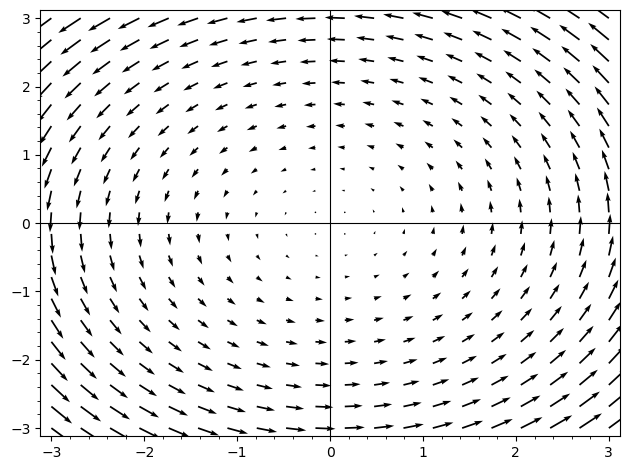
\includegraphics[scale=0.5]{Figures/vfieldex1}
$$\vcF(x,y)=\bmat{-y\\x} $$
\end{center}
\end{example}

\begin{example}{A Gradient Vector Field}
Let $f(x,y)=\sqrt{1-x^2-y^2}$. You should recognize this surface as the top half of the sphere with radius 1. But we can find $\nabla f$ and plot that as a $2$-dimensional vector field.
\begin{align*}
\nabla f=&\bmat{\delx{}(\sqrt{1-x^2-y^2})\\ \dely{}(\sqrt{1-x^2-y^2})}\\
=&\bmat{-\frac{x}{\sqrt{1-x^2-y^2}}\\-\frac{y}{\sqrt{1-x^2-y^2}}}.
\end{align*}
Then we can graph $\nabla f$ as a vector field:
\vspace{1em}
\begin{center}
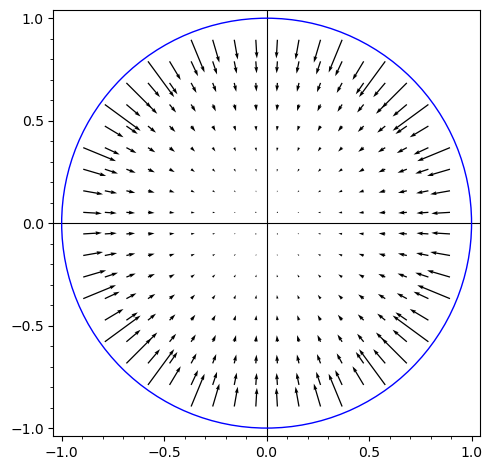
\includegraphics[scale=0.5]{Figures/gradvfieldex}\\
Gradient Vector Field for $f(x,y)=\sqrt{1-x^2-y^2}$.
\end{center}
\vspace{1em}
When referring to a vector field that comes from the gradient of a function, that is some $\vcF=\nabla f$, then $\vcF$ is the \textbf{gradient field} and $f$ is the \textbf{potential function}. If $\vcF$ is a vector field such that there exists some $f$ such that $\vcF=\nabla f$, then we say that $\vcF$ is a \textbf{conservative} vector field.
\end{example}

\begin{exercise}{Vector Fields}
For the following vector fields, generate a graph that has at least 5 vectors. You choose the points!
\vspace{1em}
\begin{enumerate}
\item $\vcF(x,y)=\bmat{2x\\-2}$.
\vspace{1em}
\item $\vcF(x,y)=\bmat{y-1\\x+y}$.
\end{enumerate}
\end{exercise}

\begin{exercise}{Gradient Vector Fields}
For the following functions, give the associated gradient vector field.
\vspace{1em}
\begin{enumerate}
\item $f(x,y)=y^2\cos(2x-y)$.
\vspace{1em}
\item $f(x,y,z)=xze^{y}$.
\end{enumerate}
\end{exercise}

\subsection{Curl and Finding Potentials}
When thinking about vector fields, we have a couple of operators on vector fields that give us useful characteristics of a given vector field. The first of these two operators is \textbf{curl}.

The curl of a vector field is a function that gives the ``rotational tendency" of the vector field at each point in the vector field. That is, if $\vcF$ is the velocity field of a fluid, then $\curl\vcF$ measures the tendency for particles to rotate about the axis that points in the direction of $\curl\vcF$. The direction of curl in 3-space is often visualized with a right hand rule-- if the thumb of your right hand points in the direction of $\curl(\vcF)$, then particles will rotate in the directions that your fingers curl around your palm. For 2-dimensional vector fields, curl always measures the tendency to rotate about a vector normal to the $xy$-plane, and so measures counterclockwise rotation if positive and clockwise if negative.

\begin{definition}{Curl}
The curl of a $3$-dimensional vector field $$\vcF(x,y,z)=\bmat{P(x,y,z)\\Q(x,y,z)\\R(x,y,z)}$$ can be calculated as $$\curl \vcF=\nabla\times\vcF =\det\bmat{\vci & \vcj & \vck \\ \delx{} & \dely{} & \frac{\del}{\del z}\\ P&Q&R}$$ where $$\det\bmat{\vci & \vcj & \vck \\ \delx{} & \dely{} & \frac{\del}{\del z}\\ P&Q&R}=\bmat{\dely{R} - \delz{Q}\\[6pt] \delz{P}-\delx{R}\\[6pt] \delx{Q}-\dely{P}}. $$
For a 2-dimensional vector field, $$\vcF(x,y)=\bmat{P(x,y)\\Q(x,y)}, $$ curl can be defined as $$\curl \vcF=\nabla\times\vcF=\det\bmat{\delx{} & \dely{}\\ P& Q}, $$ which yields $$\curl \vcF=\delx{Q}-\dely{P}.$$
\end{definition}

\begin{example}{Curl in 2 Dimensions}
Consider the vector field $$\vcF(x,y)=\bmat{-y\\x}. $$
Then we can compute $\curl\vcF$:
\begin{align*}
\nabla\times\vcF=&\det\bmat{\delx{}&\dely{}\\ -y& x}\\
=&\delx{}(x)-\dely{}(-y)\\
=&1-(-1)\\
=&2.
\end{align*}
This should line up with the \hyperlink{curl2}{vector field} that we saw earlier-- the positive curl tells us that our particles would be rotating in the counterclockwise direction.
\end{example}

\begin{exercise}{Computing Curl}
For the following vector fields, compute the curl of the vector field.
\vspace{1em}
\begin{enumerate}
\item $\vcF(x,y)=\bmat{y-1\\x+y}$.
\vspace{1em}
\item $\vcF(x,y,z)=\bmat{x^2y\\xyz\\z-3}$.
\end{enumerate}
\end{exercise}

\begin{claim}{Curl of Gradient Fields}
If $f(x,y,z)$ has continuous second partials, then $\curl(\nabla f)=\vzero$.
\end{claim}

\begin{exercise}{What?}
Prove the above claim. Hint: Work through the definition and note that continuous second partials means that \hyperlink{cs}{Clairaut-Schwarz} applies.
\end{exercise}

\begin{claim}{$\curl\vcF=\vzero \iff$ $\vcF$ is Conservative}
The previous claim tells us that if $\vcF$ is conservative, then $\curl\vcF=\vzero$. It is much harder to prove, but we will accept as fact, that if $\curl\vcF=\vzero$, then $\vcF$ is conservative. That is, if $\curl\vcF=\vzero$, then there exists a potential function $f$ such that $\nabla f=\vcF$. 
\end{claim}

\begin{example}{Finding a Potential Function}
Let's consider the vector field, $$\vcF=\bmat{2xy^2-2x\\2x^2y-2y}. $$
First, let's compute $\curl\vcF$. 
\begin{align*}
\nabla\times\vcF=&\det\bmat{\delx{}& \dely{}\\2xy^2-2x&2x^2y-2y}\\
=&\delx{}\left(2x^2y-2y\right)-\dely{}\left(2xy^2-2x\right)\\
=&4xy-4xy\\
=&0
\end{align*}
Because $\curl\vcF=0$, we know that $\vcF$ is conservative. Can we find a function $f$ such that $\nabla f=\vcF$?

\vspace{1em}

Well, we know the following:
\begin{align*}
\delx{f}=&2xy^2-2x\\
\dely{f}=&2x^2y-2y
\end{align*}
Note that the fundamental theorem of calculus tells us in the single variable case that: $$\int \frac{df}{dx}\ dx=f(x)+c. $$ However, when we integrate the partial with respect to $x$ of some $f(x,y)$ with respect to $x$, the ``constant" term can really be any function of $y$. That is, $$\int \delx{f} \ dx=f(x,y)+g(y) $$ where $g(y)$ is some unknown function of $y$. And similarly, $$\int\dely{f}\ dy=f(x,y)+h(x) $$ where $h(x)$ is some unknown function of $x$. These two integrals should allow us to piece together some $f(x,y)$ up to an unknown constant term.
\begin{align*}
\int\delx{f}\ dx=&\int2xy^2-2x\ dx\\
f(x,y)=&x^2y^2-x^2+g(y).\\
\int\dely{f}\ dy=&\int2x^2y-2y\ dy\\
f(x,y)=&x^2y^2-y^2+h(x).
\end{align*}
Then we know that $g(y)=-y^2+c_1$ and $h(x)=-x^2+c_2$, so we can find our potential function, $$f(x,y)=x^2y^2-x^2-y^2+c.$$
\end{example}

This method may seem familiar to those of you who have taken Differential Equations. That's because this is almost \textit{exactly} the same method you used for finding the solution (or potential function) to an exact differential equation. For more on this connection, check out this \href{https://youtu.be/cBoF59YyH3Q}{video}.

\begin{exercise}{Finding Potentials}
Given the following vector fields, decide if $\vcF$ is conservative. If it is, find a potential function such that $\nabla f=\vcF$.
\vspace{1em}
\begin{enumerate}
\item $\vcF=\bmat{3x^2y^2-2xy-y^2+3\\2x^3y-x^2+3y^2-2xy}$.
\vspace{1em}
\item $\vcF=\bmat{xy\cos(xy)\\x^2\cos(xy)}$.
\vspace{1em}
\item $\vcF=\bmat{yz+3x^2\\xz+2y\\xy+1}$.
\end{enumerate}
\end{exercise}

% The second operator we want to consider in this section is the \textbf{divergence} operator. Where curl can be thought of as the cross product between the gradient operator and the vector field, that is $\curl\vcF=\nabla\times\vcF$, the divergence of a vector field can be thought of as the \textit{dot product} between the gradient operator and the vector field, that is, $\divo\vcF=\nabla\bullet\vcF$.

% \begin{definition}{Div in 3 Dimensions}
% Consider the vector field $\vcF$, where $$\vcF(x,y,z)=\bmat{P(x,y,z)\\Q(x,y,z)\\R(x,y,z)}. $$
% Then $\divo\vcF=\nabla\bullet\vcf$, and can be evaluated as $$\delx{P}+\dely{Q}+\delz{R} $$
% \end{definition}

\subsection{Line Integrals}
Why do vector fields matter? What can we do with them? Consider the classic physics example of work done lifting an object. When near the surface of the earth, gravity is nearly constant, so the elementary formula work equals force times distance can be used simply. However, if we are lifting an object with varying mass or moving an object very far away from the surface of the earth we need to apply an integral to account for the changing forces. To add even another level of complexity, if you consider something like a rocket going into orbit, we can compute the amount of work by modeling the gravitational forces as a vector field and integrating across a path through said vector field. These types of integrals, where we integrate a vector field over some line, are called \textbf{line integrals}.

\begin{definition}{Line Integrals}
Let $C$ be a smooth curve in $\bbr^n$ of finite length parameterized by $$r(t), \ a\leq t\leq b.$$ Let $\vcT$ be the unit tangent vector to $\vcr(t)$. Let $\vcF$ be a vector field  $\bbr^n\to\bbr^n$. Then the line integral of $\vcF$ over $C$ is the integral of the projection of $\vcF$ onto $\vcT$ at each point along $C$, that is, $$\int_C \vcF \ d\vcr=\int_C \proj{\vcF}{\vcT} \ ds.$$
This line integral can be evaluated 
$$\int_C \proj{\vcF}{\vcT} \ ds=\int_a^b \vcF(\vcr(t))\bullet\vcr\vprime(t)\ dt.$$
\end{definition}

\begin{example}{\hypertarget{ftli}{Line Integrals}}
Consider the vector field $$\vcF=\bmat{y+1\\x} $$ and the curve $C$ parameterized by $$\vcr(t)=\bmat{\cos(t)\\ \sin(t)}, \ 0\leq t\leq\pi/2. $$
Then the line integral can be computed as 
\begin{align*}
\int_C \vcF \ d\vcr=&\int_{0}^{\pi/2}\vcF(\vcr(t))\bullet\vcr\vprime(t)\ dt\\
=&\int_{0}^{\pi/2}\bmat{\sin(t)+1\\ \cos(t)}\bullet\bmat{-\sin(t)\\\cos(t)}\ dt\\
=&\int_{0}^{\pi/2}-\sin^2(t)-\sin(t)+\cos^2(t)\ dt\\
=&\int_{0}^{\pi/2}\cos(2t)-\sin(t)\ dt\\
=&\Bigg[\frac{\sin(2t)}{2}+\cos(t)\Bigg]_{t=0}^{t=\pi/2}\\
=&\frac{\sin(\pi)}{2}+\cos(\pi/2)-\left(\frac{\sin(0)}{2}+\cos(0)\right)\\
=& 0+0-(0+1)\\
=&-1.
\end{align*}
The vector field and curve that we integrated over are graphed below-- note that our curve is oriented counterclockwise.
\vspace{1em}
\begin{center}
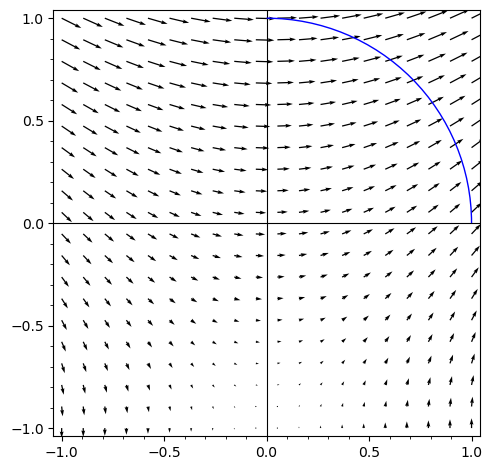
\includegraphics[scale=0.5]{Figures/lineintex}\\
Vector field and Curve (in blue).
\end{center}
\end{example}

\begin{exercise}{Doing It Backwards}
Take the same vector field and curve, but this time orient the curve clockwise. That is, let $$\vcF=\bmat{y+1\\x} $$ as before, but let $$\vcr(t)=\bmat{\sin(t)\\ \cos(t)}, \ 0\leq t\leq \pi/2$$ instead. Note: Our previous parameterization went from $(1,0)$ at $t=0$ to $(0,1)$ at $t=\pi/2$, while this parameterization goes from $(0,1)$ at $t=0$ to $(1,0)$ at $t=\pi/2$.
\end{exercise}

\begin{pexercise}{3 Dimensional}
Let $$\vcF=\bmat{8x^2yz\\5z\\-4xy}$$ and let $C$ be the curve parameterized by $$C=\left\{\vcr(t):\ \vcr(t)=\bmat{t\\t^2\\t^3},\ 0\leq t\leq 1\right\}. $$ Find $$\int_C \vcF \ dr.$$
\end{pexercise}

An important application of line integrals is finding the work it takes to move an object through a vector field. 

\begin{example}{Physics and non-parameterized curves}
Let $$\vcF=\bmat{5y\\10x}$$ and $$c=\left\{\vcr(t):\ \vcr(t)=\bmat{t\\ t^2/2},\ 0\leq t\leq 2 \right\}.$$
Then the work is equal to the line integral of $c$ over $\vcF$, or $$\int_C \vcF \ d\vcr. $$
We can evaluate this as 
\begin{align*}
\int_C\vcF \ d\vcr=&\int_0^2 \vcF(\vcr(t))\bullet\vcr\vprime(t)\ dt \\
=&\int_0^2 \bmat{5\left(t^2/2\right)\\10(t)}\bullet\bmat{1\\t}\ dt\\
=&\int_0^2\bmat{2.5t^2\\10t}\bullet\bmat{1\\ t} \ dt\\
=&\int_0^2 (2.5t^2)(1)+(10t)(t)\ dt\\
=&\int_0^2 12.5t^2\ dt\\
=&12.5\frac{t^3}{3}\Bigg]_0^2\\
=&\frac{100}{3}.
\end{align*}

\end{example}
\subsection{The Fundamental Theorem of Line Integrals}
Recall the Fundamental Theorem of Calculus-- specifically the bit that's helpful when finding definite integrals.

\begin{theorem}{Fundamental Theorem of Calculus}
Let $f(x)$ be a piecewise continuous and differentiable function on $[a,b]$ and $F(x)$ be an antiderivative of $f(x)$. Then $$\int_{a}^{b}f(x)\ dx=F(b)-F(a).$$
\end{theorem}

This momentous theorem allows for relatively easy evaluation of integrals. We have a similar style of theorem for line integrals called the \textbf{Fundamental Theorem of Line Integrals}, sometimes abbreviated as FTLI. Much like the Fundamental Theorem of Calculus allows us to evaluate integrals by just looking at their endpoints, the Fundamental Theorem of Line Integrals allows us to evaluate line integrals by just looking at their endpoints (in certain situations.)

\begin{theorem}{Fundamental Theorem of Line Integrals}
Let $C$ be a smooth curve parameterized by $\vcr(t)$, $a\leq t\leq b$. Let $f$ be a function such that $\nabla f$ is continuous over $C$. Then
$$\int_C \nabla f \ dr=f\big(\vcr(b)\big)-f(\big(\vcr(a)\big). $$
\end{theorem}

FTLI states that over a conservative vector field, we need only know the potential function and the end points of the curve to evaluate a line integral. 

\begin{example}{Doing it forwards... with FTLI!}
Lets look back at the \hyperlink{ftli}{same integral} we did in the last section. That is, consider the vector field $$\vcF=\bmat{y+1\\x} $$ and the curve $C$ parameterized by $$\vcr(t)=\bmat{\cos(t)\\ \sin(t)},\ 0\leq t\leq \frac{\pi}{2}.$$
First, note that this vector field is in fact conservative. We can compute the curl,
\begin{align*}
\nabla\times\vcF=&\det\bmat{\delx{}&\dely{}\\ y+1&x}\\
=&\delx{}(x)-\dely{}(y+1)\\
=&1-1\\
=&0
\end{align*}
Since $\curl\vcF=0$, we know the vector field is conservative. We can find the potential function by examining the antiderivatives of the respective components: 
\begin{align*}
\int y+1\ dx=&xy+x+g(y)\\
\int x \ dy=&xy+h(x).
\end{align*}
This yields a potential function $f=xy+x$. Then our line integral can be computed using FTLI:
\begin{align*}
\int_C\nabla f\ dr=& f(\cos(\pi/2),\sin(\pi/2))-f(\cos(0),\sin(0))\\
=&f(0,1)-f(1,0)\\
=&(0)(1)+0-((1)(0)+1)\\
=&-1.
\end{align*}
\end{example}

Note that an important consequence of FTLI is that line integrals over conservative vector fields are \textit{independant of path}. That is, it doesn't actually matter what $C$ is, as long as the vector field is continuous along a smooth curve, you need only the end points.

\begin{theorem}{FTLI, Take 2}
Let $C$ be a smooth curve from $(x_1,y_1)$ to $(x_2,y_2)$, and $\vcF$ be a conservative vector field that is continuous on $C$ with potential $f$. Then $$\int_C \vcF \ dr=f(x_2,y_2)-f(x_1,y_1). $$ 
\end{theorem}

\begin{exercise}{Try It Out}
For the following line integrals, verify that FTLI holds and then evaluate using FTLI.
\vspace{1em}
\begin{enumerate}
\item Let $\vcF=\nabla f$, $f=3xy+2e^x$, and $C$ be parameterized as $$C=\left\{\vcr(t):\ \vcr(t)=\bmat{t^2\\t},\ 0\leq t\leq 2 \right\}. $$ Evaluate $$\int_C\vcF\ dr.$$
\item Let $$\vcF=\bmat{2xy-y^2\\x^2-2xy} $$ and $$C=\left\{\vcr(t):\ \vcr(t)=(2t+1)\vci-t^2\vcj,\ 0\leq t\leq 3  \right\}.$$ Evaluate $$\int_C \vcF \ dr.$$
\item Let $$\vcF=\bmat{2xy^2z-e^x\\z+2x^2yz\\y+x^2y^2} $$ and $C$ be any path from $(0,0,0)$ to $(1, 4, -2)$. Evaluate $$\int_C \vcF\ dr. $$
\end{enumerate}

\end{exercise}

\begin{claim}{A Corollary to FTLI}
Let $C$ be a closed path, that is $C$ is a path that begins and ends at the same point. Then if $\vcF$ is a continuous, conservative vector field, $$\int_C \vcF \ dr=0. $$
\end{claim}

\begin{exercise}{Prove It!}
Prove the above claim.
\end{exercise}
\subsection{Green's Theorem}

Green's Theorem is an important relationship between line integrals of closed paths and double integrals.

\begin{theorem}{Green's Theorem}
Let $C$ be a closed, positively oriented, piecewise smooth, simple, curve. Let $D$ be the region enclosed by $C$, and let $\vcF$ be a 2-dimensional vector field with continuous first partials on $D$. Then $$\int_C \vcF \ dr=\iint_D\curl \vcF\ dA.$$
\end{theorem}

Note: The requirements on $C$ are as follows:
\begin{itemize}
\item \textbf{Closed}: The curve $C$ must begin and end at the same point. That is, it forms a loop.
\item \textbf{Positively Oriented}: The curve $C$ is oriented in the counter-clockwise direction.
\item \textbf{Piecewise Smooth}: The curve $C$ consists of some countable amount of smooth subcurves. A curve is smooth if it has no jumps or holes or cusps (though cusps are allowed between different subcurves of $C$).
\item \textbf{Simple}: The curve $C$ does not cross over itself.
\end{itemize}

Let's try and build a little intuition around Green's Theorem. The left hand side of the theorem is a line integral of a closed curve over some vector field. Essentially, what it is doing is it is measuring how well the vector field ``travels" with the curve. Another way of saying that is that it measures how well $\vcF$ circulates around $C$. 

The right hand side, on the other hand, is the double integral of the curl of $\vcF$ over the region enclosed by $C$. The curl of $\vcF$ essentially measures the clockwise circulation at a given point of $\vcF$, and by taking a double integral over the region, we are essentially accumulating the total circulation of the entire region of $D$.

So Green's theorem asserts that the total circulation of $\vcF$ in the region $D$ (the right hand side) is equal to the circulation of $\vcF$ on the \textit{boundary} of $D$, $C$ (the left hand side). Why is this true? Well, lets take a region, $D$. Here, it will be a square for simplicity.

\begin{center}
\begin{tikzpicture}[scale=2]
\draw [thick] (0,0)--(0,2)--(2,2)--(2,0)--(0,0);
\node (1) at (1,1) {$D$};
\end{tikzpicture}
\end{center}

Suppose we want to measure $\iint_D\curl\vcF\ dr$. Then we're essentially breaking $D$ up into smaller and smaller subregions, and measuring the curl of each of those subregions. Technically the double integral breaks the region up into infintesimally small squares, but we'll just break it up into 4 squares.

\begin{center}
\begin{tikzpicture}[scale=2]
%\draw [thick] (-0.05,-0.05)--(-0.05,2.05)--(2.05,2.05)--(2.05,-0.05)--(-0.05,-0.05);
\draw [thick] (0.05,0.05)--(0.95,0.05)--(0.95,0.95)--(0.05,0.95)--(0.05,0.05);
\draw [thick] (1.05,0.05)--(1.95,0.05)--(1.95,0.95)--(1.05,0.95)--(1.05,0.05);
\draw [thick] (1.05,1.05)--(1.95,1.05)--(1.95,1.95)--(1.05,1.95)--(1.05,1.05);
\draw [thick] (0.05,1.05)--(0.95,1.05)--(0.95,1.95)--(0.05,1.95)--(0.05,1.05);
%\node (1) at (1,1) {$D$};
\end{tikzpicture}
\end{center}

Then we can measure the curl around each of those four regions, which is the counter clockwise circulation.

\begin{center}
\begin{tikzpicture}[scale=2]
%\draw [thick] (0,0)--(0,2)--(2,2)--(2,0)--(0,0);
%\draw [thick] (-0.05,-0.05)--(-0.05,2.05)--(2.05,2.05)--(2.05,-0.05)--(-0.05,-0.05);
\draw [-stealth,thick](0.05,0.05)--(0.95,0.05);
\draw [-stealth,thick](0.95,0.05)--(0.95,0.95);
\draw [-stealth,thick](0.95,0.95)--(0.05,0.95);
\draw [-stealth,thick](0.05,0.95)--(0.05,0.05);

\draw [-stealth,thick](1.05,0.05)--(1.95,0.05);
\draw [-stealth,thick](1.95,0.05)--(1.95,0.95);
\draw [-stealth,thick](1.95,0.95)--(1.05,0.95);
\draw [-stealth,thick](1.05,0.95)--(1.05,0.05);

\draw [-stealth,thick](1.05,1.05)--(1.95,1.05);
\draw [-stealth,thick](1.95,1.05)--(1.95,1.95);
\draw [-stealth,thick](1.95,1.95)--(1.05,1.95);
\draw [-stealth,thick](1.05,1.95)--(1.05,1.05);

\draw [-stealth,thick](0.05,1.05)--(0.95,1.05);
\draw [-stealth,thick](0.95,1.05)--(0.95,1.95);
\draw [-stealth,thick](0.95,1.95)--(0.05,1.95);
\draw [-stealth,thick](0.05,1.95)--(0.05,1.05);
%\node (1) at (1,1) {$D$};
\end{tikzpicture}
\end{center}

We can continue breaking the regions down into smaller and smaller subregions if we want.

\begin{center}
\begin{tikzpicture}[scale=2]
%\draw [thick] (0,0)--(0,2)--(2,2)--(2,0)--(0,0);
%\draw [thick] (-0.05,-0.05)--(-0.05,2.05)--(2.05,2.05)--(2.05,-0.05)--(-0.05,-0.05);
\draw [-stealth,thick](0.05,0.05)--(0.45,0.05);
\draw [-stealth,thick](0.45,0.05)--(0.45,0.45);
\draw [-stealth,thick](0.45,0.45)--(0.05,0.45);
\draw [-stealth,thick](0.05,0.45)--(0.05,0.05);

\draw [-stealth,thick](0.05,0.55)--(0.45,0.55);
\draw [-stealth,thick](0.45,0.55)--(0.45,0.95);
\draw [-stealth,thick](0.45,0.95)--(0.05,0.95);
\draw [-stealth,thick](0.05,0.95)--(0.05,0.55);

\draw [-stealth,thick](0.55,0.05)--(0.95,0.05);
\draw [-stealth,thick](0.95,0.05)--(0.95,0.45);
\draw [-stealth,thick](0.95,0.45)--(0.55,0.45);
\draw [-stealth,thick](0.55,0.45)--(0.55,0.05);

\draw [-stealth,thick](0.55,0.55)--(0.95,0.55);
\draw [-stealth,thick](0.95,0.55)--(0.95,0.95);
\draw [-stealth,thick](0.95,0.95)--(0.55,0.95);
\draw [-stealth,thick](0.55,0.95)--(0.55,0.55);


\draw [-stealth,thick](1.05,0.05)--(1.45,0.05);
\draw [-stealth,thick](1.45,0.05)--(1.45,0.45);
\draw [-stealth,thick](1.45,0.45)--(1.05,0.45);
\draw [-stealth,thick](1.05,0.45)--(1.05,0.05);

\draw [-stealth,thick](1.05,0.55)--(1.45,0.55);
\draw [-stealth,thick](1.45,0.55)--(1.45,0.95);
\draw [-stealth,thick](1.45,0.95)--(1.05,0.95);
\draw [-stealth,thick](1.05,0.95)--(1.05,0.55);

\draw [-stealth,thick](1.55,0.05)--(1.95,0.05);
\draw [-stealth,thick](1.95,0.05)--(1.95,0.45);
\draw [-stealth,thick](1.95,0.45)--(1.55,0.45);
\draw [-stealth,thick](1.55,0.45)--(1.55,0.05);

\draw [-stealth,thick](1.55,0.55)--(1.95,0.55);
\draw [-stealth,thick](1.95,0.55)--(1.95,0.95);
\draw [-stealth,thick](1.95,0.95)--(1.55,0.95);
\draw [-stealth,thick](1.55,0.95)--(1.55,0.55);


\draw [-stealth,thick](0.05,1.05)--(0.45,1.05);
\draw [-stealth,thick](0.45,1.05)--(0.45,1.45);
\draw [-stealth,thick](0.45,1.45)--(0.05,1.45);
\draw [-stealth,thick](0.05,1.45)--(0.05,1.05);

\draw [-stealth,thick](0.05,1.55)--(0.45,1.55);
\draw [-stealth,thick](0.45,1.55)--(0.45,1.95);
\draw [-stealth,thick](0.45,1.95)--(0.05,1.95);
\draw [-stealth,thick](0.05,1.95)--(0.05,1.55);

\draw [-stealth,thick](0.55,1.05)--(0.95,1.05);
\draw [-stealth,thick](0.95,1.05)--(0.95,1.45);
\draw [-stealth,thick](0.95,1.45)--(0.55,1.45);
\draw [-stealth,thick](0.55,1.45)--(0.55,1.05);

\draw [-stealth,thick](0.55,1.55)--(0.95,1.55);
\draw [-stealth,thick](0.95,1.55)--(0.95,1.95);
\draw [-stealth,thick](0.95,1.95)--(0.55,1.95);
\draw [-stealth,thick](0.55,1.95)--(0.55,1.55);


\draw [-stealth,thick](1.05,1.05)--(1.45,1.05);
\draw [-stealth,thick](1.45,1.05)--(1.45,1.45);
\draw [-stealth,thick](1.45,1.45)--(1.05,1.45);
\draw [-stealth,thick](1.05,1.45)--(1.05,1.05);

\draw [-stealth,thick](1.05,1.55)--(1.45,1.55);
\draw [-stealth,thick](1.45,1.55)--(1.45,1.95);
\draw [-stealth,thick](1.45,1.95)--(1.05,1.95);
\draw [-stealth,thick](1.05,1.95)--(1.05,1.55);

\draw [-stealth,thick](1.55,1.05)--(1.95,1.05);
\draw [-stealth,thick](1.95,1.05)--(1.95,1.45);
\draw [-stealth,thick](1.95,1.45)--(1.55,1.45);
\draw [-stealth,thick](1.55,1.45)--(1.55,1.05);

\draw [-stealth,thick](1.55,1.55)--(1.95,1.55);
\draw [-stealth,thick](1.95,1.55)--(1.95,1.95);
\draw [-stealth,thick](1.95,1.95)--(1.55,1.95);
\draw [-stealth,thick](1.55,1.95)--(1.55,1.55);

%\node (1) at (1,1) {$D$};
\end{tikzpicture}
\end{center}

We can continue doing this until we have infinitesimally small subregions. Then when we look at the curl on two adjacent subregions we see that the shared edge of the subregion has equal and opposite rotational tendency. When accumulating the total rotation, these edges cancel, leaving us with just the rotational tendency about the border of the pair.

\begin{center}
\begin{tikzpicture}[scale=2]
%\draw [thick] (0,0)--(0,2)--(2,2)--(2,0)--(0,0);
%\draw [thick] (-0.05,-0.05)--(-0.05,2.05)--(2.05,2.05)--(2.05,-0.05)--(-0.05,-0.05);
\draw [-stealth,thick](0.05,0.05)--(0.95,0.05);
\draw [-stealth,thick,red](0.95,0.05)--(0.95,0.95);
\draw [-stealth,thick](0.95,0.95)--(0.05,0.95);
\draw [-stealth,thick](0.05,0.95)--(0.05,0.05);

\draw [-stealth,thick](1.05,0.05)--(1.95,0.05);
\draw [-stealth,thick](1.95,0.05)--(1.95,0.95);
\draw [-stealth,thick](1.95,0.95)--(1.05,0.95);
\draw [-stealth,thick,red](1.05,0.95)--(1.05,0.05);
%\node (1) at (1,1) {$D$};
\node(=) at (2.5,0.5) {$=$};

\draw [-stealth,thick](3.05,0.05)--(4,0.05);
%\draw [-stealth,thick](3.95,0.05)--(3.95,0.95);
\draw [-stealth,thick](4,0.95)--(3.05,0.95);
\draw [-stealth,thick](3.05,0.95)--(3.05,0.05);

\draw [-stealth,thick](4,0.05)--(4.95,0.05);
\draw [-stealth,thick](4.95,0.05)--(4.95,0.95);
\draw [-stealth,thick](4.95,0.95)--(4,0.95);
%\draw [-stealth,thick](4.05,0.95)--(4.05,0.05);
\end{tikzpicture}
\end{center}

We can expand this out and cancel equal and opposite pairs as necessary.

\begin{center}
\begin{tikzpicture}[scale=2]
%\draw [thick] (0,0)--(0,2)--(2,2)--(2,0)--(0,0);
%\draw [thick] (-0.05,-0.05)--(-0.05,2.05)--(2.05,2.05)--(2.05,-0.05)--(-0.05,-0.05);
\draw [-stealth,thick](0.05,0.05)--(0.45,0.05);
\draw [-stealth,thick,red](0.45,0.05)--(0.45,0.45);
\draw [-stealth,thick,red](0.45,0.45)--(0.05,0.45);
\draw [-stealth,thick](0.05,0.45)--(0.05,0.05);

\draw [-stealth,thick,red](0.05,0.55)--(0.45,0.55);
\draw [-stealth,thick,red](0.45,0.55)--(0.45,0.95);
\draw [-stealth,thick,red](0.45,0.95)--(0.05,0.95);
\draw [-stealth,thick](0.05,0.95)--(0.05,0.55);

\draw [-stealth,thick](0.55,0.05)--(0.95,0.05);
\draw [-stealth,thick,red](0.95,0.05)--(0.95,0.45);
\draw [-stealth,thick,red](0.95,0.45)--(0.55,0.45);
\draw [-stealth,thick,red](0.55,0.45)--(0.55,0.05);

\draw [-stealth,thick,red](0.55,0.55)--(0.95,0.55);
\draw [-stealth,thick,red](0.95,0.55)--(0.95,0.95);
\draw [-stealth,thick,red](0.95,0.95)--(0.55,0.95);
\draw [-stealth,thick,red](0.55,0.95)--(0.55,0.55);


\draw [-stealth,thick](1.05,0.05)--(1.45,0.05);
\draw [-stealth,thick,red](1.45,0.05)--(1.45,0.45);
\draw [-stealth,thick,red](1.45,0.45)--(1.05,0.45);
\draw [-stealth,thick,red](1.05,0.45)--(1.05,0.05);

\draw [-stealth,thick,red](1.05,0.55)--(1.45,0.55);
\draw [-stealth,thick,red](1.45,0.55)--(1.45,0.95);
\draw [-stealth,thick,red](1.45,0.95)--(1.05,0.95);
\draw [-stealth,thick,red](1.05,0.95)--(1.05,0.55);

\draw [-stealth,thick](1.55,0.05)--(1.95,0.05);
\draw [-stealth,thick](1.95,0.05)--(1.95,0.45);
\draw [-stealth,thick,red](1.95,0.45)--(1.55,0.45);
\draw [-stealth,thick,red](1.55,0.45)--(1.55,0.05);

\draw [-stealth,thick,red](1.55,0.55)--(1.95,0.55);
\draw [-stealth,thick](1.95,0.55)--(1.95,0.95);
\draw [-stealth,thick,red](1.95,0.95)--(1.55,0.95);
\draw [-stealth,thick,red](1.55,0.95)--(1.55,0.55);


\draw [-stealth,thick,red](0.05,1.05)--(0.45,1.05);
\draw [-stealth,thick,red](0.45,1.05)--(0.45,1.45);
\draw [-stealth,thick,red](0.45,1.45)--(0.05,1.45);
\draw [-stealth,thick](0.05,1.45)--(0.05,1.05);

\draw [-stealth,thick,red](0.05,1.55)--(0.45,1.55);
\draw [-stealth,thick,red](0.45,1.55)--(0.45,1.95);
\draw [-stealth,thick](0.45,1.95)--(0.05,1.95);
\draw [-stealth,thick](0.05,1.95)--(0.05,1.55);

\draw [-stealth,thick,red](0.55,1.05)--(0.95,1.05);
\draw [-stealth,thick,red](0.95,1.05)--(0.95,1.45);
\draw [-stealth,thick,red](0.95,1.45)--(0.55,1.45);
\draw [-stealth,thick,red](0.55,1.45)--(0.55,1.05);

\draw [-stealth,thick,red](0.55,1.55)--(0.95,1.55);
\draw [-stealth,thick,red](0.95,1.55)--(0.95,1.95);
\draw [-stealth,thick](0.95,1.95)--(0.55,1.95);
\draw [-stealth,thick,red](0.55,1.95)--(0.55,1.55);


\draw [-stealth,thick,red](1.05,1.05)--(1.45,1.05);
\draw [-stealth,thick,red](1.45,1.05)--(1.45,1.45);
\draw [-stealth,thick,red](1.45,1.45)--(1.05,1.45);
\draw [-stealth,thick,red](1.05,1.45)--(1.05,1.05);

\draw [-stealth,thick,red](1.05,1.55)--(1.45,1.55);
\draw [-stealth,thick,red](1.45,1.55)--(1.45,1.95);
\draw [-stealth,thick](1.45,1.95)--(1.05,1.95);
\draw [-stealth,thick,red](1.05,1.95)--(1.05,1.55);

\draw [-stealth,thick,red](1.55,1.05)--(1.95,1.05);
\draw [-stealth,thick](1.95,1.05)--(1.95,1.45);
\draw [-stealth,thick,red](1.95,1.45)--(1.55,1.45);
\draw [-stealth,thick,red](1.55,1.45)--(1.55,1.05);

\draw [-stealth,thick,red](1.55,1.55)--(1.95,1.55);
\draw [-stealth,thick](1.95,1.55)--(1.95,1.95);
\draw [-stealth,thick](1.95,1.95)--(1.55,1.95);
\draw [-stealth,thick,red](1.55,1.95)--(1.55,1.55);

%\node (1) at (1,1) {$D$};
\end{tikzpicture}
\end{center}

After cancelling, we're left with just the circulation about the boundary.

\begin{center}
\begin{tikzpicture}[scale=2]
%\draw [thick] (0,0)--(0,2)--(2,2)--(2,0)--(0,0);
%\draw [thick] (-0.05,-0.05)--(-0.05,2.05)--(2.05,2.05)--(2.05,-0.05)--(-0.05,-0.05);
\draw [-stealth,thick](0.05,0.05)--(0.45,0.05);
%\draw [-stealth,thick,red](0.45,0.05)--(0.45,0.45);
%\draw [-stealth,thick,red](0.45,0.45)--(0.05,0.45);
\draw [-stealth,thick](0.05,0.45)--(0.05,0.05);

%\draw [-stealth,thick,red](0.05,0.55)--(0.45,0.55);
%\draw [-stealth,thick,red](0.45,0.55)--(0.45,0.95);
%\draw [-stealth,thick,red](0.45,0.95)--(0.05,0.95);
\draw [-stealth,thick](0.05,0.95)--(0.05,0.55);

\draw [-stealth,thick](0.55,0.05)--(0.95,0.05);
%\draw [-stealth,thick,red](0.95,0.05)--(0.95,0.45);
%\draw [-stealth,thick,red](0.95,0.45)--(0.55,0.45);
%\draw [-stealth,thick,red](0.55,0.45)--(0.55,0.05);

%\draw [-stealth,thick,red](0.55,0.55)--(0.95,0.55);
%\draw [-stealth,thick,red](0.95,0.55)--(0.95,0.95);
%\draw [-stealth,thick,red](0.95,0.95)--(0.55,0.95);
%\draw [-stealth,thick,red](0.55,0.95)--(0.55,0.55);


\draw [-stealth,thick](1.05,0.05)--(1.45,0.05);
%\draw [-stealth,thick,red](1.45,0.05)--(1.45,0.45);
%\draw [-stealth,thick,red](1.45,0.45)--(1.05,0.45);
%\draw [-stealth,thick,red](1.05,0.45)--(1.05,0.05);

%\draw [-stealth,thick,red](1.05,0.55)--(1.45,0.55);
%\draw [-stealth,thick,red](1.45,0.55)--(1.45,0.95);
%\draw [-stealth,thick,red](1.45,0.95)--(1.05,0.95);
%\draw [-stealth,thick,red](1.05,0.95)--(1.05,0.55);

\draw [-stealth,thick](1.55,0.05)--(1.95,0.05);
\draw [-stealth,thick](1.95,0.05)--(1.95,0.45);
%\draw [-stealth,thick,red](1.95,0.45)--(1.55,0.45);
%\draw [-stealth,thick,red](1.55,0.45)--(1.55,0.05);

%\draw [-stealth,thick,red](1.55,0.55)--(1.95,0.55);
\draw [-stealth,thick](1.95,0.55)--(1.95,0.95);
%\draw [-stealth,thick,red](1.95,0.95)--(1.55,0.95);
%\draw [-stealth,thick,red](1.55,0.95)--(1.55,0.55);


%\draw [-stealth,thick,red](0.05,1.05)--(0.45,1.05);
%\draw [-stealth,thick,red](0.45,1.05)--(0.45,1.45);
%\draw [-stealth,thick,red](0.45,1.45)--(0.05,1.45);
\draw [-stealth,thick](0.05,1.45)--(0.05,1.05);

%\draw [-stealth,thick,red](0.05,1.55)--(0.45,1.55);
%\draw [-stealth,thick,red](0.45,1.55)--(0.45,1.95);
\draw [-stealth,thick](0.45,1.95)--(0.05,1.95);
\draw [-stealth,thick](0.05,1.95)--(0.05,1.55);

%\draw [-stealth,thick,red](0.55,1.05)--(0.95,1.05);
%\draw [-stealth,thick,red](0.95,1.05)--(0.95,1.45);
%\draw [-stealth,thick,red](0.95,1.45)--(0.55,1.45);
%\draw [-stealth,thick,red](0.55,1.45)--(0.55,1.05);

%\draw [-stealth,thick,red](0.55,1.55)--(0.95,1.55);
%\draw [-stealth,thick,red](0.95,1.55)--(0.95,1.95);
\draw [-stealth,thick](0.95,1.95)--(0.55,1.95);
%\draw [-stealth,thick,red](0.55,1.95)--(0.55,1.55);


%\draw [-stealth,thick,red](1.05,1.05)--(1.45,1.05);
%\draw [-stealth,thick,red](1.45,1.05)--(1.45,1.45);
%\draw [-stealth,thick,red](1.45,1.45)--(1.05,1.45);
%\draw [-stealth,thick,red](1.05,1.45)--(1.05,1.05);

%\draw [-stealth,thick,red](1.05,1.55)--(1.45,1.55);
%\draw [-stealth,thick,red](1.45,1.55)--(1.45,1.95);
\draw [-stealth,thick](1.45,1.95)--(1.05,1.95);
%\draw [-stealth,thick,red](1.05,1.95)--(1.05,1.55);

%\draw [-stealth,thick,red](1.55,1.05)--(1.95,1.05);
\draw [-stealth,thick](1.95,1.05)--(1.95,1.45);
%\draw [-stealth,thick,red](1.95,1.45)--(1.55,1.45);
%\draw [-stealth,thick,red](1.55,1.45)--(1.55,1.05);

%\draw [-stealth,thick,red](1.55,1.55)--(1.95,1.55);
\draw [-stealth,thick](1.95,1.55)--(1.95,1.95);
\draw [-stealth,thick](1.95,1.95)--(1.55,1.95);
%\draw [-stealth,thick,red](1.55,1.95)--(1.55,1.55);

\node (1) at (1,1) {$D$};
\end{tikzpicture}
\end{center}

This is exactly the line integral, $$\int_{C}\vcF \ dr. $$

Green's theorem is a good example of a theorem where both directions are useful. For example, sometimes you have a line integral on a curve that would require an annoying parameterization, but the region that's enclosed is actually quite easy to describe.

\begin{example}{An Annoying Line Integral}
Let $\vcF=\bmat{xy\\-x}$. Let $C$ be the positively oriented rectangle with a corner at $(0,0)$ and $(1,1)$.

\begin{center}
\begin{tikzpicture}[scale=2]
\draw (-0.5,0)--(1.5,0);
\draw (0,-0.5)--(0,1.5);
\draw [-stealth,thick] (0,0)--(1,0);
\draw [-stealth,thick] (1,0)--(1,1);
\draw [-stealth,thick] (1,1)--(0,1);
\draw [-stealth,thick] (0,1)--(0,0);
\draw [gray] (1,0.05)--(1,-0.05);
%\draw [gray] (-1,0.05)--(-1,-0.05);
%\draw [gray] (2,0.05)--(2,-0.05);
\draw [gray] (0.05,1)--(-0.05,1);
%\draw [gray] (0.05,2)--(-0.05,2);
%\draw [gray] (0.05,-1)--(-0.05,-1);
\end{tikzpicture}\\
The positively oriented path, $C$.
\end{center}

Suppose we wanted to evaluate $$\int_C \vcF \ dr. $$ 

To evaluate this line integral, it would be necessary to actually parameterize our line integrals over four separate sections. That is, we could define:
\begin{align*}
C_1=&\left\{\vcr_1(t):\ \vcr_1(t)=\bmat{t\\0}, \ 0\leq t\leq 1 \right\}\\
C_2=&\left\{\vcr_2(t):\ \vcr_2(t)=\bmat{1\\t-1}, \ 1\leq t\leq 2 \right\}\\
C_3=&\left\{\vcr_3(t):\ \vcr_3(t)=\bmat{3-t\\1}, \ 2\leq t\leq 3 \right\}\\
C_4=&\left\{\vcr_4(t):\ \vcr_4(t)=\bmat{0\\4-t}, \ 3\leq t\leq 4 \right\}
\end{align*}
Then we could evaluate:
$$\int_C \vcF \ dr=\int_{C_1} \vcF \ dr+\int_{C_2} \vcF \ dr+\int_{C_3} \vcF \ dr+\int_{C_4} \vcF \ dr.$$
\end{example}

\begin{exercise}{A Piecewise Line Integral}
Find $$\int_C \vcF \ dr=\int_{C_1} \vcF \ dr+\int_{C_2} \vcF \ dr+\int_{C_3} \vcF \ dr+\int_{C_4} \vcF \ dr$$ using the parameterization from the example above.
\end{exercise}

\begin{exercise}{Green's Theorem to the Rescue}
Use Green's theorem to rewrite the integral from the previous problem as a double integral, then solve.
\end{exercise}

\begin{exercise}{Nephroid, Area by Line Integral}
If you roll a circle of radius 1 around a circle of radius 2, then fix a point on the circle of radius 1, that point traces out the curve known as the \textit{nephroid.}

\vspace{1em}

\begin{center}
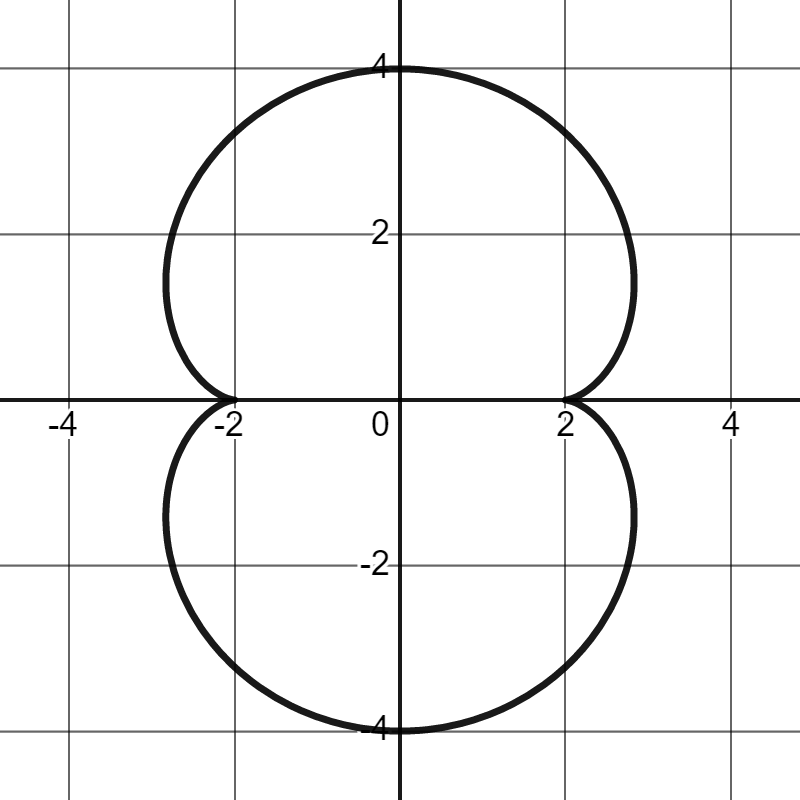
\includegraphics[scale=0.25]{Figures/nephroid}\\
Visit \href{https://www.desmos.com/calculator/a8o5rvqufn}{Desmos} to see the nephroid traced out.
\end{center}

\vspace{1em}

Call the region enclosed by the nephroid $R$. Then we could compute the area of the nephroid as $$\iint_R 1 \ dA.$$
Unfortunately, parameterizing the nephroid as a function is quite annoying, so instead we will try to apply Green's Theorem to evaluate the area using a line integral. Let $$\vcF=\bmat{0\\x}, $$ a vector field chosen specifically because it has a curl of $1$. Then $$\iint_R 1 \ dA =\iint_R \curl\vcF \ dA.$$ With this clever choice of $\vcF$, Green's Theorem applies, which means that we can evaluate this area using a \textbf{line integral.}

\vspace{1em}

Use the fact that the nephroid curve can be parameterized as $$\vcr(t)=\bmat{3\cos(t)-\cos(3t)\\3\sin(t)-\sin(3t)},\ 0\leq t\leq 2\pi$$ and Green's Theorem to verify that the area of the nephroid is $12\pi$. Note that the resulting integral you get here can be solved using the triple angle identities:
\begin{align*}
\sin(3\theta)&=3\sin(\theta)-4\sin^3(\theta),\\
\cos(3\theta)&=4\cos^3(\theta)-3\cos(\theta).
\end{align*}
\end{exercise}

\begin{exercise}{Sine Flowers}
Consider the region $R$ inside the polar function $r=\sin(2\theta)$, where $0\leq\theta\leq \frac{\pi}{2}$. Find the area of $R$ in two ways.

\vspace{1em}
\begin{enumerate}
\item Using a double integral, $$\iint_R 1\ dA.$$ Hint: You probably want to convert to polar coordinates.
\vspace{1em}
\item Using a line integral $$\int_C \vcF\ dr $$ where $$\vcF=\bmat{0\\x}\text{ and }C=\vcr(t)=\bmat{2\sin(t)\cos^2(t)\\2\sin^2(t)\cos(t)},\ 0\leq t\leq \frac{\pi}{2}.$$ This integral can be done by hand, but is relatively long, so feel free to use a CAS to solve.
\end{enumerate}
\end{exercise}
\renewcommand\thesubsection{\thesection.\Alph{subsection}}
\setcounter{subsection}{18}
\subsection{Line Integrals Summary}
\begin{definition}{Vector Fields}
\begin{itemize}
\item \textbf{2-d Vector Field:} $$\vcF(x,y)=\bmat{P(x,y)\\Q(x,y)}. $$
\item \textbf{3-d Vector Field:}$$\vcF(x,y,z)=\bmat{P(x,y,z)\\Q(x,y,z)\\R(x,y,z)}. $$
\end{itemize}
If $f$ is a function from $\bbr^n\to\bbr$, the gradient of $f$ is an $n$-d vector field, i.e. $\nabla f=\vcF$.
\end{definition}

\begin{definition}{Curl}
\begin{itemize}
\item \textbf{2-d Curl:} $$\curl \vcF=\delx{Q}-\dely{P}.$$
\item \textbf{3-d Curl:} $$\curl \vcF=\nabla\times\vcF =\det\bmat{\vci & \vcj & \vck \\ \delx{} & \dely{} & \frac{\del}{\del z}\\ P&Q&R}.$$ 
\end{itemize}
\end{definition}

\begin{definition}{Conservative Vector Fields}
A vector field, $\vcF$ is conservative if and only if there exists some potential function $f$ such that $\nabla f=\vcF$.

\vspace{1em}

A vector field, $\vcF$ is conservative if and only if $\curl\vcF=\vzero$.
\end{definition}

\begin{definition}{Finding a Potential}
Let $\vcF=\bmat{P(x,y)\\Q(x,y)}$ be conservative. Then there exists some $f(x,y)$ such that:
\begin{align*}
f(x,y)=&\int P(x,y)\ dx\\
=&f_1(x,y)+g(y)\\
f(x,y)=&\int Q(x,y)\ dy\\
=&f_2(x,y)+h(x).
\end{align*}
\end{definition}

\begin{definition}{Line Integral}
$$\int_C \vcF \ d\vcr=\int_a^b \vcF\big(\vcr(t)\big)\bullet\vcr\vprime(t)\ dt. $$
\end{definition}

\begin{theorem}{FTLI Ver. 1}
Let $C$ be a smooth curve parameterized by $\vcr(t)$, $a\leq t\leq b$. Let $f$ be a function such that $\nabla f$ is continuous over $C$. Then
$$\int_C \nabla f \ dr=f\big(\vcr(b)\big)-f(\big(\vcr(a)\big). $$
\end{theorem}

\begin{theorem}{FTLI Ver. 2}
Let $C$ be a smooth curve from $(x_1,y_1)$ to $(x_2,y_2)$, and $\vcF$ be a conservative vector field that is continuous on $C$ with potential $f$. Then $$\int_C \vcF \ dr=f(x_2,y_2)-f(x_1,y_1). $$ 
\end{theorem}

\begin{theorem}{Green's Theorem}
Let $C$ be a closed, positively oriented, piecewise smooth, simple, curve. Let $D$ be the region enclosed by $C$, and let $\vcF$ be a 2-dimensional vector field with continuous first partials on $D$. Then $$\int_C \vcF \ dr=\iint_D\curl \vcF\ dA.$$
\end{theorem}

\renewcommand\thesubsection{\thesection.\arabic{subsection}}
\renewcommand\thesubsection{\thesection.\Alph{subsection}}
\setcounter{subsection}{17}
\subsection{Line Integrals Homework and Miscellaneous Practice}


\begin{exercise}{Curl 1}
Let $\vcF=\bmat{x\sin(y)\\y\cos(x)}$. Compute $\curl\vcF$.
\end{exercise}

\begin{pexercise}{Curl 2}
Let $\vcF=\bmat{x^2y\\3x-z^3\\4y^2}$. Compute $\curl\vcF$.
\end{pexercise}

\begin{exercise}{Potential 1}
Let $\vcF=\bmat{2x\sin(2y)-3y^2\\2-6xy+2x^2\cos(2y)}$ Is $\vcF$ conservative? If yes, find the potential function.
\end{exercise}

\begin{exercise}{Potential 2}
Let $\vcF=\bmat{yz+2xy+2xz\\xz+x^2+2yz\\xy+x^2+y^2}$ Is $\vcF$ conservative? If yes, find the potential function.
\end{exercise}

\begin{exercise}{Line Integral}
Let $\vcF=\bmat{-y\\x}$ and let $C$ be parameterized by $\vcr(t)=\bmat{t\\t^2}$, $0\leq t\leq 1$. Find $$\int_C \vcF \ dr. $$
\end{exercise}

\begin{pexercise}{FTLI 1}
Let $f(x,y)=x^3(3-y)+4y$ and $C$ be parameterized by $\vcr(t)=\bmat{3-t^2\\5-2}$, $-2\leq t\leq 3$. Find $$\int_C \nabla f \ dr.$$
\end{pexercise}

\begin{exercise}{FTLI 2}
Let $\vcF=\bmat{yz\\xz\\xy}$ and $C$ be any path from $(0,0,0)$ to $(1,1,1)$. Verify that FTLI applies, then evaluate $$\int_C \vcF \ dr. $$
\end{exercise}

\begin{exercise}{Green's 1}
Let $\vcF=\bmat{y-\cos x\\e^y-2x}$ be a vector field that represents a force. Suppose a particle moves through that field counterclockwise in a circle of radius 3, starting and ending at $(3,0)$. Use Green's theorem to evaluate the work done on the particle, $$\int_C \vcF \ dr.$$
\end{exercise}

\begin{exercise}{Green's 2}
Find the area of a circle of radius $r$ with a line integral by using Green's Theorem, where $\vcF=\bmat{-y/2\\x/2}$ and $\vcr(t)=\bmat{r\cos t\\ r\sin t}$, $0\leq t\leq 2\pi$.
\end{exercise}
\renewcommand\thesubsection{\thesection.\arabic{subsection}}

\section{Surface Integrals}
\subsection{Parameterization of Surfaces}
Remember that early in the semester we dealt with parametric equations. Specifically, we dealt with \hyperlink{paraderiv}{parametric curves} in 3-dimensional space. However, we primarily dealt functions from $\bbr\to\bbr^3$, that is, functions with a single input that yielded a vector output, a 1-dimensional object in 3-dimensional space. However, we can also consider parametric surfaces, functions from $\bbr^2\to\bbr^3$, that yield 2-dimensional objects in 3-dimensional space. We briefly dealt with this topic when covering the \hyperlink{paraplane}{parametric form of a plane}.

\begin{definition}{Parametric Surface}
Let $\vcr(u,v)$ be a function from $\bbr^2\to\bbr^3$, where $$\vcr(u,v)=\bmat{x(u,v)\\y(u,v)\\z(u,v)}.$$ The outputs vector valued function as a set of points in $\bbr^3$ defines a parametric surface $S$ in $3$-dimensional space.
\end{definition}

Note that we can actually consider any of the \hyperlink{surf1}{surfaces} we looked at in the second part of this class as parametric surfaces.

\begin{example}{A Surface, Parameterized}
Let $f(x,y)=10-x^2+y^3-3y^2-6y$. Then we can parameterize this surface by letting $x(u,v)=u$, $y(u,v)=v$, and $z(u,v)=f(u,v)$. Then we get the parameterization $$\vcr(u,v)=\bmat{u\\v\\10-u^2+v^3-3v^2-6v}.$$
\end{example}

\begin{exercise}{Identifying and Parameterizing Surfaces}
\begin{enumerate}
\item Consider the parametric surface $$\vcr(\theta,\phi)=\bmat{4\sin(\phi)\cos(\theta)\\4\sin(\phi)\sin(\theta)\\4(\cos(\phi)}.$$ What does this surface represent? Hint: Consider the \hyperlink{spherical}{spherical transformation for triple integrals}.
\vspace{1em}
\item Parameterize a cylinder with radius of 3 where the cross sections parallel to the $xy$-plane are circles. (i.e. it's height runs parallel to the $z$ axis). Hint: Consider the \hyperlink{cylind}{cylindrical transformation for triple integrals}.
\end{enumerate}
\end{exercise}

We can also find planes tangent to parametric surfaces. We'll use partial derivatives, much like we did before, so let's state what the partial derivative of a parametric surface is.

\begin{definition}{Partial Derivative of a Parametric Surface}
Let $$\vcr(u,v)=\bmat{x(u,v)\\y(u,v)\\z(u,v)}$$ be a parametric surface where $x,y,z$ are differentiable functions. Then define the partial derivatives as \begin{align*}
\vcr_u(u,v)=&\bmat{\frac{\del}{\del u}\big(x(u,v)\big)\\\frac{\del}{\del u}\big(y(u,v)\big)\\\frac{\del}{\del u}\big(z(u,v)\big)}=\bmat{x_u(u,v)\\y_u(u,v)\\z_u(u,v)}\\
\vcr_v(u,v)=&\bmat{\frac{\del}{\del v}\big(x(u,v)\big)\\\frac{\del}{\del v}\big(y(u,v)\big)\\\frac{\del}{\del v}\big(z(u,v)\big)}=\bmat{x_v(u,v)\\y_v(u,v)\\z_v(u,v)}
\end{align*}
\end{definition}

Note that if we take some $\vcr(u,v)$ and some fixed point on the surface $(u_0,v_0)$, then $\vcr(u,v_0)$ and $\vcr(u_0,v)$ are both parametric curves that pass through the point $(u_0,v_0)$. Then $\vcr_u(u_0,v_0)$ gives a vector tangent to $\vcr(u,v_0)$ at $(u_0,v_0)$, and $\vcr_v(u_0,v_0)$ gives a vector tangent to $\vcr(u_0,v)$ at $(u_0,v_0)$. These two vectors should be independent from each other and parallel to the plane tangent to $\vcr(u,v)$ at $(u_0,v_0)$, so we can generate the equation of the plane by using the cross product of the two derivatives to find a normal vector!

\begin{example}{Tangent Plane}
Consider the parametric surface $S$, parameterized by $$\vcr(u,v)=\bmat{4\sin(u)\cos(v)\\4\sin(u)\sin(v)\\4\cos(u)}.$$ From before, we know this represents a sphere of radius 4, centered at the origin. Let's find the plane tangent to $S$ at $u=\frac{\pi}{6}$ and $v=\frac{\pi}{6}$. 
\vspace{1em}
\begin{center}
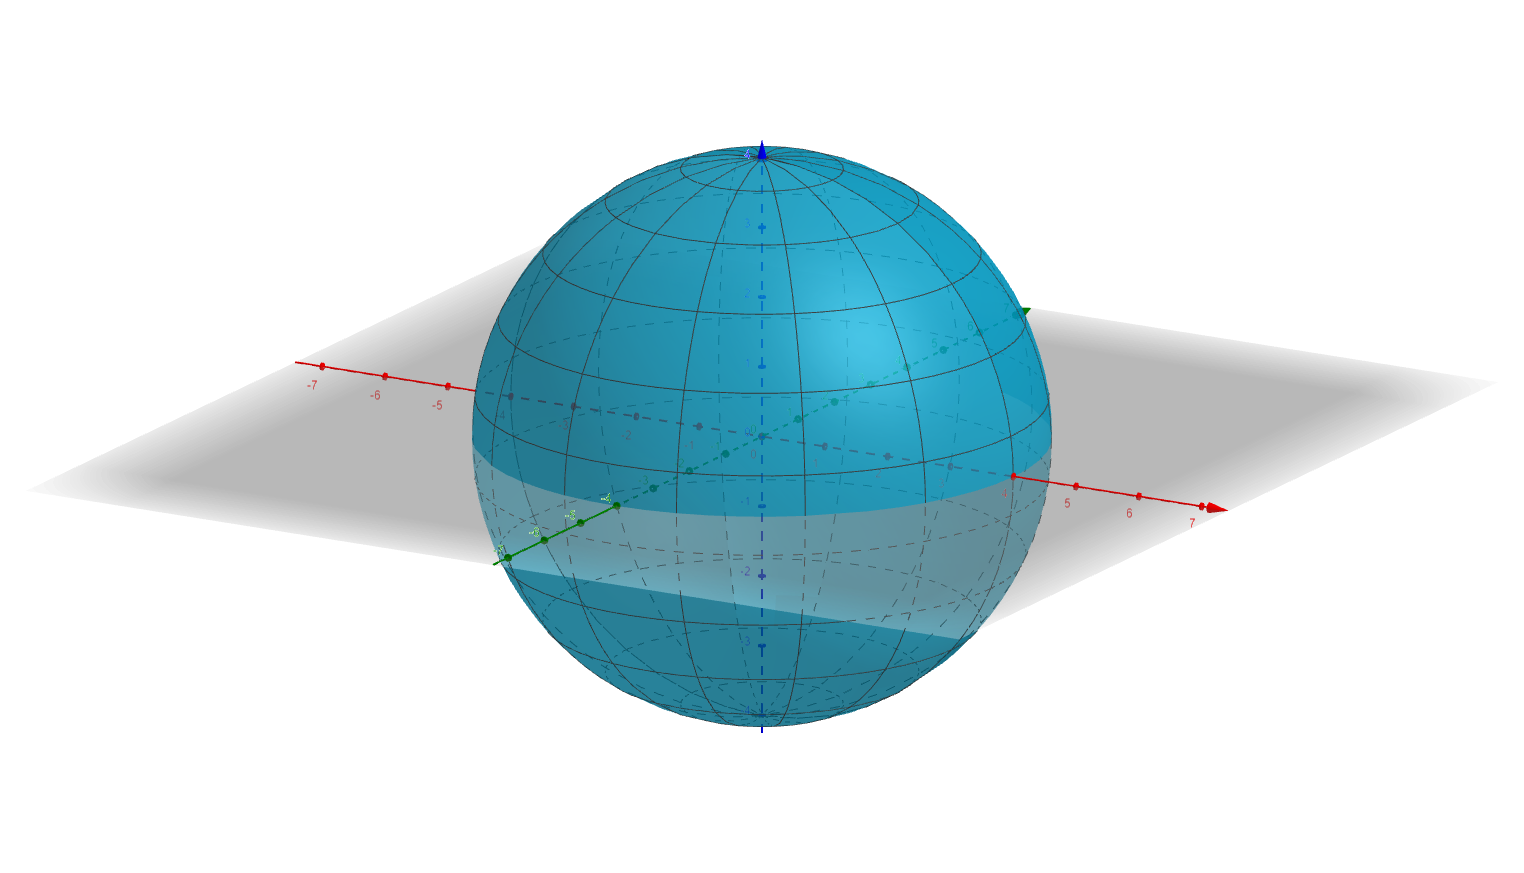
\includegraphics[scale=0.3]{Figures/sphere}\\
The surface $S$ (\href{https://www.geogebra.org/3d/hmgt3b7w}{Geogebra Link}).
\end{center}
\vspace{1em}
To find the tangent plane, we'll first need to find our two partial derivatives.
\begin{align*}
\vcr_u(u,v)=&\bmat{4\cos(u)\cos(v)\\4\cos(u)\sin(v)\\-4\sin(u)}\\
\vcr_v(u,v)=&\bmat{-4\sin(u)\sin(v)\\4\sin(u)\cos(v)\\0}\\
\end{align*}
Then we can plug in our values, which yields:
$$\vcr_u\left(\frac{\pi}{6},\frac{\pi}{6} \right)=\bmat{3\\ \sqrt{3}\\-2},\ \vcr_v\left(\frac{\pi}{6},\frac{\pi}{6} \right)=\bmat{-1\\ \sqrt{3}\\0}.$$
\begin{center}
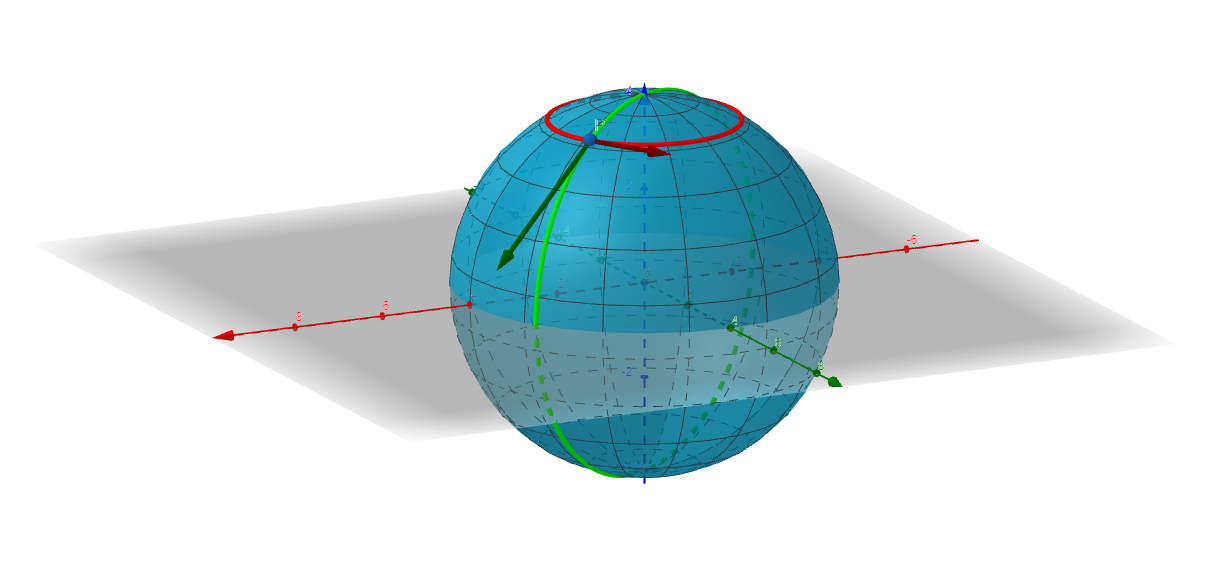
\includegraphics[scale=0.3]{Figures/surftan}\\
The surface $S$ with tangent vectors (\href{https://www.geogebra.org/3d/s78y49td}{Geogebra Link}).
\end{center}
\vspace{1em}
Then we can cross these two tangent vectors together to get the normal vector to our plane.
\begin{align*}\vcr_u\left(\frac{\pi}{6},\frac{\pi}{6} \right)\times\vcr_v\left(\frac{\pi}{6},\frac{\pi}{6} \right)=&\bmat{3\\ \sqrt{3}\\-2}\times\bmat{-1\\ \sqrt{3}\\0}\\
=&\det\bmat{\vci&\vcj&\vck\\3&\sqrt{3}&-2\\-1&\sqrt{3}&0}\\
=&\bmat{2\sqrt{3}\\2\\4\sqrt{3}}.
\end{align*}
Now we need only the coordinates of our point on the curve as $(x,y,z)$, which we find by evaluating $\vcr(u,v)$ at $u=\frac{\pi}{6}$ and $v=\frac{\pi}{6}$
$$\vcr\left(\frac{\pi}{6},\frac{\pi}{6} \right)=\bmat{\sqrt{3}\\1\\\ 2\sqrt{3}}. $$
Then we can use vector dot product form to generate the equation of our plane, then simplify to standard form.
\begin{align*}
2\sqrt{3}(x-\sqrt{3})+2(y-1)+4\sqrt{3}(z-2\sqrt{3})=&0\\
2\sqrt{3}x-6+2y-2+4\sqrt{3}z-24=&0\\
2\sqrt{3}x+2y+4\sqrt{3}z=&32\\
\sqrt{3}x+y+2\sqrt{3}z=&16.
\end{align*}\begin{center}
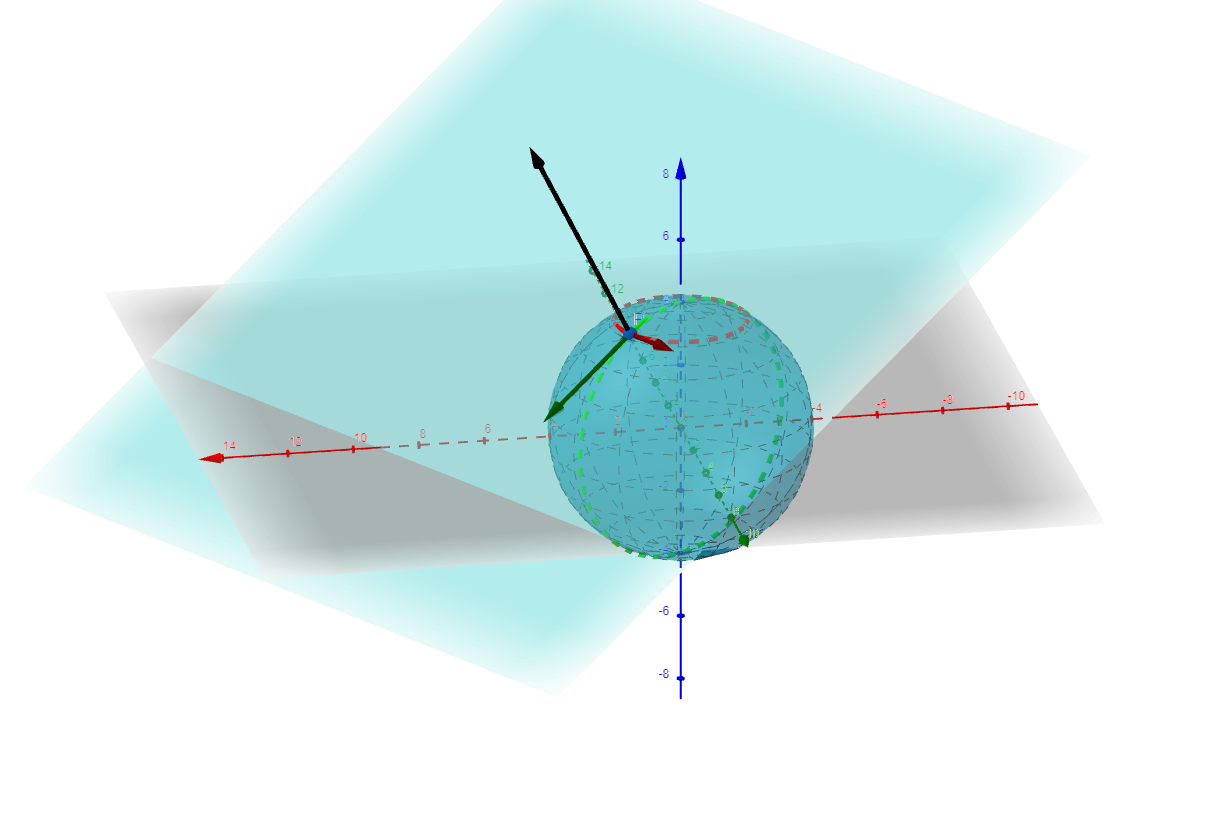
\includegraphics[scale=0.3]{Figures/surftan3}\\
The surface $S$ with tangent plane (\href{https://www.geogebra.org/3d/psngscyc}{Geogebra Link}).
\end{center}
\end{example}

\begin{exercise}{Is it a Bird? No, it's a Tangent Plane.}
\begin{enumerate}
\item Find the plane tangent to the \href{https://www.geogebra.org/3d/ympnc8vk}{surface $S$} parameterized by $$\vcr(u,v)=\bmat{u-4\\v^2\\u^2-2u+1}$$ at $u=2$, $v=1$.
\vspace{1em}
\item Find the plane tangent to the \href{https://www.geogebra.org/3d/dkmxdxkq}{surface $S$} parameterized by $$\vcr(u,v)=\bmat{v\\2\cos(u)\\2\sin(u)}$$ at $u=\frac{\pi}{4}$, $v=2$.
\end{enumerate}
\end{exercise}
\subsection{Surface Integrals}
We now visit \textbf{surface integrals}, a generalization of multiple integrals to integration over surfaces. The surface integral is to double integrals as the line integral is to single integrals. Much like we defined the line integral in terms of a single integral, we'll define the surface integral in terms of a double integral.

\begin{definition}{Surface Integral of a Parametric Surface}
Let $S$ be a surface parameterized by $\vcr(u,v)$ with $(u,v)$ over some region $R$. Then we define the surface integral $$\iint_S \ dS $$ as the area of that surface over the region $R$. The surface integral can be evaluated as $$\iint_S \ dS= \iint_R ||\vcr_u\times\vcr_v||\ dA.$$
\end{definition}
\begin{exercise}{Is That Really Surface Area?}
Let $S$ be a surface parameterized by $$\vcr(x,y)=\bmat{x\\y\\f(x,y)}$$ with $(x,y)$ in some region $R$. Show that the above surface area integral is equivalent to the integral given \hyperlink{surfarea}{last unit}. That is, show: $$\iint_R ||\vcr_x\times\vcr_y||\ dA=\iint_R \sqrt{(f_x)^2+(f_y)^2+1}\ dA. $$
\end{exercise}
\begin{exercise}{The Surface Area of a Sphere... Again}
Let $S$ be the sphere with radius 1 centered at the origin, parameterized as: $$\vcr(\phi,\theta)=\bmat{\sin(\phi)\cos(\theta)\\\sin(\phi)\sin(\theta)\\\cos(\phi)} $$ where $0\leq \phi\leq\pi$ and $0\leq \theta\leq 2\pi$. Compute the surface area of the sphere using a surface integral: $$\iint_S \ dS =\iint_R ||\vcr_\phi\times\vcr_\theta||\ dA.$$
\end{exercise}

Surface integrals go a little further than this though-- in fact, the analogy between surface integrals and line integrals extends to the fact that they are most interesting over vector fields. 

Recall that a line integral essentially computes how ``aligned" with a given vector field a trajectory is. If we thought of a vector field as a force field and the curve as a trajectory that a particle moves along, then a positive line integral meant that the vector field helps the particle along and a negative line integral meant that the vector field was hindering the particle's movement.

The metaphor for a surface integral is more like that of a ``sail". Essentially, given a surface in a vector field, the surface integral measures how much the vector field pushes that surface along it's normal vector. Essentially, at each point along the surface we project the vector field onto the normal vector of the surface at that point, then the integral accumulates all of the different projections.

\begin{definition}{Surface Integral of a Parametric Surface over a Vector Field}
Let $S$ be a smooth surface in $\bbr^3$ parameterized by $\vcr(u,v)$ with $(u,v)$ in some region $R$. Let $\vcF$ be a vector field. Let $\vcn$ be the unit normal vector function to $S$, that is, $$\vcn=\frac{\vcr_u\times\vcr_v}{||\vcr_u\times\vcr_v||}.$$ Then the surface integral $$\iint_S \vcF \ d\vec{S} $$ can be computed as follows: 
\begin{align*}
\iint_S \vcF \ d\vec{S} =&\iint_S ||\proj{\vcF}{\vcn} || \ dS\\
=&\hyperlink{unitproj}{\iint_S \vcF\bullet\vcn \ dS}\\
=&\iint_S \frac{\vcF\bullet(\vcr_u\times\vcr_v)}{||\vcr_u\times\vcr_v||}\ dS\\
=&\iint_R \frac{\vcF\bullet(\vcr_u\times\vcr_v)}{||\vcr_u\times\vcr_v||}||\vcr_u\times\vcr_v||\ dA\\
\iint_S \vcF \ d\vec{S} =&\iint_R \vcF\big(\vcr(u,v)\big)\bullet(\vcr_u\times\vcr_v)\ dA.
\end{align*}
\end{definition}

Note-- the sign of the result depends entirely on the \textbf{orientation} of the surface. When you're finding a normal vector to a surface, both $\vcr_u\times\vcr_v$ and $\vcr_v\times\vcr_u$ provide normal vectors. However, since the cross product is \hyperlink{crossprop}{antisymmetric}, the choice of orientation comes down to the choice of cross product. For a non-closed surface, there's nothing to really prefer one orientation over the other necessarily. However, if the surface is closed (e.g. a sphere), then we say that the surface is \textbf{positively oriented} if the normal vectors point away from the interior.

\begin{exercise}{more sphere}
Let $$\vcF=\bmat{x\\y\\z}$$ and let $S$ be the upper half of the unit sphere, parameterized by $$\vcr(\phi,\theta)=\bmat{\sin(\phi)\cos(\theta)\\\sin(\phi)\sin(\theta)\\\cos(\phi)}, $$ where $0\leq\phi\leq \pi/2$ and $0\leq \theta\leq 2\pi$. Compute $$\iint_S \vcF\ d\vcS. $$
\end{exercise}

\begin{exercise}{Surface Integral of $f(x,y)$}
Let $S$ be a smooth surface in $\bbr^3$, $z=f(x,y)$ over the region $R$. We can parameterize this surface as $$\vcr(x,y)=\bmat{x\\y\\f(x,y)}.$$ Let $\vcF$ be a 3-dimensional vector field. Show that $$\iint_S \vcF \ d\vcS=\iint_R \vcF\bullet \bmat{-f_x\\-f_y\\1}\ dA.$$
\end{exercise}

\begin{pexercise}{Another Surface Integral}
Let $$\vcF=\bmat{3x\\2z\\1-y^2}, $$ and let $S$ be the portion of $f(x,y)=2-3y+x^2$ that lies over the triangle in the $xy$-plane with vertices $(0,0)$, $(2,0)$ and $(2,-4)$. 
\end{pexercise}
\subsection{Divergence Theorem}
We visited an important operator on vector fields earlier in the curl operator. Here, we visit its companion, divergence. Where $\curl \vcF$ measures the tendency to rotate clockwise about a given vector at a point in a vector field, $\divo \vcF$ measures the tendency to diverge away from a given point in a vector field. A positive divergence means that the rate of flow out of the point is higher than the rate of flow into a point. Of course, with most incompressible fluids like water, this is impossible. In fact, in these types of \textbf{incompressible} fields, $\divo\vcF=0$.

\begin{definition}{Divergence}
Let $\vcF$ be a vector field. Then the divergence of $\vcF$ can be calculated as
$$\divo\vcF=\nabla\bullet\vcF.$$
If $\vcF$ is a 3-dimensional vector field, $$\vcF=\bmat{P(x,y,z)\\Q(x,y,z)\\R(x,y,z)} $$ then:
$$\divo\vcF=\nabla\bullet\vcF=\bmat{\delx{}\\ \dely{} \\ \delz{}}\bullet\bmat{P\\Q\\R}=\delx{P}+ \dely{Q}+ \delz{R} .$$
\end{definition}

\begin{exercise}{Divergence}
\begin{enumerate}
\item Let $\vcF=\bmat{x^2-y\\y\sin(z)\\z^4}$. Find $\divo\vcF$.
\vspace{1em}
\item Let $\vcF=\bmat{e^{x^2}\\xyz\\z\sec{z}}$. Find $\divo\vcF$.
\end{enumerate}
\end{exercise}

\begin{exercise}{Divergence and Curl}
Let $\vcF=\bmat{P(x,y,z)\\Q(x,y,z)\\R(x,y,z)}$, where $P$, $Q$, and $R$ have continuous second partials. Verify that $$\divo(\curl\vcF)=0.$$
\end{exercise}

In the same way that Green's Theorem relates line integrals over closed paths to double integrals of the curl of the enclosed region, the \textbf{divergence theorem} relates surface integrals of closed surfaces to triple integrals of the divergence of the enclosed region.

\begin{theorem}{Divergence Theorem}
Let $R$ be a simple solid region and $S$ be the closed surface that encloses $R$ with positive orientation. Let $F$ be a vector field with continuous first partials. Then $$\iint_S \vcF \ d\vcS=\iiint_R \divo\vcF \ dV.$$
\end{theorem}

Much like Green's theorem, the divergence theorem allows us to both compute surface integrals using triple integrals and triple integrals using surface integrals. 

\begin{exercise}{EVEN MORE SPHEEEEEEEERE}
Let $S$ be the unit sphere, parameterized as $$\vcr(\phi,\theta)=\bmat{\sin(\phi)\cos(\theta)\\\sin(\phi)\sin(\theta)\\\cos(\phi)}, \ 0\leq \phi\leq \pi,\ 0\leq\theta\leq2\pi.$$
Let $R$ be the region enclosed by $S$, and let $$\vcF=\bmat{0\\0\\z}.$$ Verify that $\divo\vcF=1$, so then the volume of the sphere can be calculated via a surface integral by way of divergence theorem, $$\iiint_R \divo\vcF \ dV=\iint_S \vcF \ d\vcS,$$ then compute the volume of the unit sphere by way of said surface integral.
\end{exercise}

Note however, surface integrals tend to be very tedious to compute, while divergence is relatively easy to compute, so more often we see divergence theorem used to translate surface integrals to triple integrals.

\begin{pexercise}{Surface to Triple}
Let $$\vcF=\bmat{\sin{(\pi x)}\\ zy^3\\z^2+4x}$$ and $S$ be the surface of the box that surrounds the rectangular prism $[-1,2]\times[0,1]\times[1,4]$ with positive orientation. Use the divergence theorem to evaluate $$\iint_S \vcF \ d\vcS $$ as a triple integral.
\end{pexercise}
\subsection{Stokes' Theorem}
While the divergence theorem is analogous to Green's theorem, Stokes' Theorem is a genuine \textit{generalization} of Green's Theorem that relates line integrals to surface integrals. Let $S$ be an oriented surface in $\bbr^3$ and let $C$ be the boundary curve of $S$ with \textit{positive orientation}. In this case, positive orientation means in the counter-clockwise direction, or as you walk along the boundary curve, the surface should be on the left hand side. Then we can state Stokes' Theorem:

\begin{theorem}{Stokes' Theorem}
Let $S$ be an oriented smooth surface that is bounded by a simple, closed, smooth boundary curve $C$ with positive orientation. Let $\vcF$ be a vector field. Then $$\int_C\vcF \ d\vcr=\iint_S\curl\vcF\ d\vcS.$$
\end{theorem}

\begin{exercise}{Generalizing Green's}
Let $S$ be a smooth surface parameterized by $$\vcr(u,v)=\bmat{x(u,v)\\y(u,v)\\0} $$ over some region $R$. Let $\vcF$ be a vector field where $$\vcF=\bmat{P(x,y)\\Q(x,y)\\0}.$$ Show that $$\iint_S \curl\vcF \ d\vcS=\iint_R\curl\vcF dA.$$ Hint: What's going on with the $z$-coordinate here? What's the difference between $R$ and $S$?
\end{exercise}

Note: Just like Green's theorem, while technically you can use Stokes' theorem in a situation with a conservative vector field, if the vector field is conservative, then $\curl\vcF=0$, so both the line integral and the surface integral should evaluate to 0.

Also worth noting-- while double integrals and line integrals are relatively similar in ``difficulty", surface integrals tend to be much more annoying than either of them. Because of this, Stokes's theorem is much more likely to reduce a surface integral to a line integral rather than the other way around.

\begin{exercise}{Surface Independence}
\begin{enumerate}
\item Let $S$ be the portion of $z=\sqrt{4-x^2-y^2} $ that is above the $xy$-plane and let $$\vcF=\bmat{z^2\\-3xy\\x^3y^3}.$$ Evaluate $$\iint_S \curl\vcF \ d\vcS $$ as a line integral using Stokes' theorem.
\vspace{1em}
\item Let $S$ be the portion of $z=16-4x^2-4y^2 $ that is above the $xy$-plane and let $$\vcF=\bmat{z^2\\-3xy\\x^3y^3}.$$ Evaluate $$\iint_S \curl\vcF \ d\vcS $$ as a line integral using Stokes' theorem.
\end{enumerate}
\end{exercise}

The previous exercise should justify that as long as the boundary curve is the same, it doesn't matter what surface you actually integrate. In this case, the ability to choose the surface can lead to a pretty tidy surface integral.

\begin{pexercise}{Another Annoying Line Integral}
Use Stokes' theorem to evaluate $$\int_C\vcF\ d\vcr $$ where $$\vcF=\bmat{z^2\\y^2\\x}$$ and $C$ is the triangle with vertices at $(1,0,0)$, $(0,1,0)$, and $(0,0,1)$. Hint: Consider the surface: $$\vcr(x,y)=\bmat{x\\y\\1-x-y},\ 0\leq x\leq 1, 0\leq y\leq 1-x $$ which is just the plane $x+y+z=1$ over the triangle with vertices at $(0,0)$, $(1,0)$ and $(0,1)$.
\end{pexercise}

\renewcommand\thesubsection{\thesection.\Alph{subsection}}
\setcounter{subsection}{18}
\subsection{Surface Integrals Summary}
\begin{definition}{Parametric Surface} $$\vcr(u,v)=\bmat{x(u,v)\\y(u,v)\\z(u,v)}.$$ 
\end{definition}

\begin{definition}{Partial Derivatives of Parametric Surfaces}
$$\vcr_u(u,v)=\bmat{x_u(u,v)\\y_u(u,v)\\z_u(u,v)}\quad\vcr_v(u,v) \bmat{x_v(u,v)\\y_v(u,v)\\z_v(u,v)} $$
\end{definition}

\begin{definition}{Tangent Plane to Parametric Surface}
The plane tangent to the surface $\vcr(u,v)$ at $u=u_0$, $v=v_0$ has normal vector $\vcr_u(u_0,v_0)\times\vcr_v(u_0,v_0)$ and passes through $\vcr(u_0,v_0)$, yielding vector-dot product form: $$\big(\vcx-\vcr(u_0,v_0)\big)\bullet\big(\vcr_u(u_0,v_0)\times\vcr_v(u_0,v_0)\big)=0. $$
\end{definition}

\begin{definition}{Surface Integral}
$$\iint_S \ dS= \iint_R ||\vcr_u\times\vcr_v||\ dA.$$
\end{definition}

\begin{definition}{Surface Integral of a Vector Field}
$$\iint_S \vcF \ d\vec{S} =\iint_R \vcF\big(\vcr(u,v)\big)\bullet(\vcr_u\times\vcr_v)\ dA$$
\end{definition}

\begin{definition}{Divergence}
$$\divo\vcF=\nabla\bullet\vcF=\delx{P}+ \dely{Q}+ \delz{R} .$$
\end{definition}

\begin{theorem}{Divergence Theorem}
Let $R$ be a simple solid region and $S$ be the closed surface that encloses $E$ with positive orientation. Let $F$ be a vector field with continuous first partials. Then $$\iint_S \vcF \ d\vcS=\iiint_R \divo\vcF \ dV.$$
\end{theorem}

\begin{theorem}{Stokes' Theorem}
Let $S$ be an oriented smooth surface that is bounded by a simple, closed, smooth boundary curve $C$ with positive orientation. Let $\vcF$ be a vector field. Then $$\int_C\vcF \ d\vcr=\iint_S\curl\vcF\ d\vcS.$$
\end{theorem}
\renewcommand\thesubsection{\thesection.\arabic{subsection}}
\renewcommand\thesubsection{\thesection.\Alph{subsection}}
\setcounter{subsection}{17}
\subsection{Surface Integrals Homework and Miscellaneous Practice}
\begin{exercise}{Tangent Plane 1}
Let $S$ be the surface parameterized by $$\vcr(u,v)=\bmat{u\cos(v)\\u\sin(v)\\\sqrt{2}u}$$ Find the plane tangent to $S$ at $u=\sqrt{2}$, $v=\frac{\pi}{4}$.
\end{exercise}

\begin{exercise}{Tangent Plane 2}
Let $S$ be the surface parameterized by $$\vcr(u,v)=\bmat{u^2\\v^2\\uv}$$ Find the plane tangent to $S$ at $u=1$, $v=1$.
\end{exercise}

\begin{pexercise}{Surface Integral 1}
Let $S$ be the section of the sphere parameterized by $$\vcr(\phi,\theta)=\bmat{3\sin\phi\cos\theta \\ 3\sin\phi\sin\theta \\ 3\cos\phi}$$ where $x\leq 0$, $y\geq 0$ and $z\geq 0$ (that is, the octant above quadrant II). Let $$\vcF=\bmat{1\\z\\6x}$$ Evaluate $$\iint \vcF\ d\vcS $$
\end{pexercise}

\begin{exercise}{Surface Integral 2}
Let $S$ be the surface parameterized by $$\vcr(u,v)=\bmat{u^2\\v^2\\uv},\ 0\leq u\leq1 ,\ 0\leq v \leq1 .  $$ Let $$\vcF=\bmat{x\\y\\z}.$$ Evaluate $$\iint \vcF \ d\vcS $$
\end{exercise}

\begin{exercise}{Divergence}
Let $$\vcF=\bmat{yx^2\\xy^2-3z^4\\x^3+y^2}. $$ Find $\divo\vcF$.
\end{exercise}

\begin{pexercise}{Divergence Theorem}
Use the divergence theorem to evaluate $$\iint_S \vcF\ d \vcS $$ where $$\vcF=\bmat{2xz\\1-4xy^2\\2z-z^2} $$ and $S$ is the surface of the solid bounded by $z=6-2x^2-2y^2$ and the $xy$-plane.
\end{pexercise}

\begin{pexercise}{Stokes' Theorem 1}
Use Stoke's theorem to evaluate $$\iint_S \curl\vcF \ d\vcS $$ where $$\vcF=\bmat{y\\-x\\yx^3} $$ and $S$ is the portion of the sphere of radius 4 centered at the origin with $z\geq 0$.
\end{pexercise}

\begin{pexercise}{Stokes' Theorem 2}
Use Stokes' theorem to evaluate $$\int_C \vcF\ d\vcr $$ where $$\vcF=\bmat{3x^2y+z^3\\y^2\\4yx^2}$$ and $C$ is a triangle with vertices $(0,0,3)$, $(0,2,0)$ and $(4,0,0)$ with a counterclockwise rotation. Hint: Remember, you can parameterize a plane $f(x,y)$ over the region $R$ as $$\vcr(x,y)=\bmat{x\\y\\f(x,y)}$$ over the same region.
\end{pexercise}

\renewcommand\thesubsection{\thesection.\arabic{subsection}}

\section*{Exam 3 Review}
\addcontentsline{toc}{section}{Exam 3 Review}
\setcounter{counter}{0}

\begin{revex}{Curl}
Let $\vcF=\bmat{x\arctan{(y)}\\y^2\\x^2z}$. Find $\curl\vcF$.
\end{revex}

\begin{revex}{Potential}
Let $\vcF=\bmat{3x^2y\\x^3\\z^2}$. Verify that $\vcF$ is conservative and find the potential for $\vcF$.
\end{revex}

\begin{revex}{Line Integral}
Let $$\vcF=\bmat{-2y\\x^2}.$$ Let $C$ be parameterized by $$\vcr(t)=\bmat{1-t\\t^2},\ 0\leq t\leq 1. $$
Evaluate $$\int_C \vcF \ d\vcr.$$
\end{revex}

\begin{revex}{FTLI 1}
Let $f(x,y)=xe^{xy}$ and let $C$ be any curve that runs between $(5,0)$ and $(0,5)$. Find $$\int_C \nabla f \ d\vcr. $$ 
\end{revex}

\begin{revex}{FTLI 2}
Let $$\vcF=\bmat{2xy\\x^2}. $$ Let $C$ be parameterized by $$\vcr(t)=\bmat{\cos(t)\\ 2\sin(t)},\ 0\leq t \leq \pi .$$
Verify that $\vcF$ is conservative and use FTLI to evaluate $$\int_C \vcF \ d\vcr. $$
\end{revex}

\begin{revex}{Green's 2}
Let $\vcF=\bmat{y^2\\x^2}$ and $C$ be the rectangle with corners at $(0,0) $, $(2,0) $, $(2,3) $, and $(0,3) $ oriented counterclockwise. Use Green's Theorem to evaluate $$\int_C \vcF \ d\vcr $$ as a double integral.
\end{revex}

\begin{revex}{Tangent Plane}
Let $S$ be the surface parameterized by $$\vcr(u,v)=\bmat{(2+\cos u)\cos v\\(2+\cos u)\sin v\\ \sin u} .$$ Find the plane tangent to $S$ at $u=\pi/4$, $v=\pi/4$.
\end{revex}

\begin{revex}{Surface Integral 1}
Let $S$ be the plane $z=1-x-y$ in the region above the first quadrant of the $xy$-plane. Find $$\iint_S \ dS.$$
\end{revex}

\begin{revex}{Surface Integral 2}
Let $$\vcF=\bmat{3x\\2z\\1-y^2}$$ and $S$ be the portion of $f(x,y)=2-3y+x^2$ that lies over the triangle in the $xy$-plane with vertices at $(0,0)$, $(2,0)$, $(2,-4)$. Evaluate $$\iint_S \vcF\ d\vcS. $$
\end{revex}

\begin{revex}{Divergence Theorem}
Let $$\vcF=\bmat{x^2\\2xy\\2xz}$$ and $S$ be the surface of the sphere with radius 3. Use Divergence theorem to evaluate $\iint_S \vcF \ d\vcS$.
\end{revex}

\begin{revex}{Stokes' 1}
Let $C$ be the intersection of $z=2-y$ and $x^2+y^2=1$. \href{https://www.geogebra.org/3d/dcdcjckt}{Geogebra Link}. Let $$\vcF=\bmat{-y^2\\x\\z^2} $$ Use Stokes' theorem to evaluate $$\int_C \vcF \ d\vcr $$ by way of a surface integral. Hint: you can use the plane $z=2-y$ as your surface, and the other object should give you an idea of the region of integration.
\end{revex}

\begin{revex}{Stokes' 2}
Let $S$ be the top half of a sphere with radius 3. Let $$\vcF=\bmat{2y\\x^2\\z}.$$ Find $$\iint_S \curl\vcF \ d \vcS $$ using a line integral by way of Stokes' theorem. $\emptyset 0 O \theta \phi$
\end{revex}



\end{document}